Find the equation of line 
\begin{enumerate}[label=\thesubsection.\arabic*, ref=\thesubsection.\theenumi]
	\item passing through the point $\vec{P} = (– 4,  3)$ with slope $\frac{1}{2}$.
\label{chapters/11/10/2/2}
\\
\solution
\begin{enumerate}[label=\thesection.\arabic*.,ref=\thesection.\theenumi]
\numberwithin{equation}{enumi}
\item The equation of a line is given by 
\begin{align}
			\label{eq:app-line-school}
	y &= mx + c
	\\
	\implies \myvec{x \\ y} &= \myvec{x \\ 
	 mx + c} =\myvec{0 \\ c} + x\myvec{1 \\ m}
\end{align}
			yielding \eqref{eq:geo-param}.
\item 			\eqref{eq:app-line-school} can also be expressed as
\begin{align}
	y - mx &= c 
	\\
	\implies \myvec{-m & 1}\myvec{x \\ y} &= c
\end{align}
			yielding \eqref{eq:geo-normal}.
		\item The direction vector is 
\begin{align}
			\label{eq:app-line-school-dir}
\vec{m} = \myvec{1 \\ m}
\end{align}
and the normal vector is
\begin{align}
\vec{n}=\myvec{-m \\ 1}
			\label{eq:app-line-school-normal}
\end{align}
  \item From \eqref{eq:geo-param}, 
	  if $\vec{A},\vec{D}$ and $\vec{C}$ are on the same line,
		\label{prop:app-lin-dep}
\begin{align}
			\vec{D}=\vec{A}+q\vec{m} 
			\\ 
			\vec{C}=\vec{D}+p\vec{m} \\
			\label{eq:app-collinear} 
			\implies 	p\brak{\vec{D}-\vec{A}} 
			+ q\brak{\vec{D}-\vec{C}} = 0, \quad p, q \ne 0 \\ 
			\implies \vec{D} = \frac{p\vec{A}+q\vec{C}}{p+q} 
			\end{align} 
			yielding \eqref{eq:section_formula} upon substituting \begin{align} k = \frac{p}{q}. \end{align} 
			$\brak{\vec{D}-\vec{A}}, \brak{\vec{D}-\vec{C}}$ 
		are then said to be {\em linearly dependent}.
	\item If $\vec{A}, \vec{B}, \vec{C}$ are collinear,  from \eqref{eq:geo-normal}, \begin{align}
	 \vec{n}^{\top}\vec{A} &=  c 
	 \\
	 \vec{n}^{\top}\vec{B} &=  c 
	 \\
	 \vec{n}^{\top}\vec{C} &=  c 
\end{align}
which can be expressed as 
\begin{align}
		\label{prop:app-lin-eq}
	\myvec{ \vec{A} & \vec{B} & \vec{C}}^{\top}\vec{n} = c\myvec{1 \\ 1 \\ 1}
	\\
	\equiv \myvec{ \vec{A} & \vec{B} & \vec{C}}^{\top}\vec{n} = \myvec{1 \\ 1 \\ 1}
		\label{prop:app-lin-eq-unit-mat},
	\\
	\implies 
	\myvec{ \vec{A} & \vec{B} & \vec{C}\\ 1 & 1 &1 }^{\top}\myvec{\vec{n} \\ -1} &= \vec{0}
		\label{prop:app-lin-dep-rank}
\end{align}
yielding
		\begin{align}
			\label{eq:app-line-rank-2}
			\rank{\myvec{1 & 1 & 1 \\ \vec{A}& \vec{B}&\vec{C}}} = 2
		\end{align}
			  Rank is defined to be the number of linearly indpendent rows or columns of a matrix.
		\item
The equation of a line can also be expressed as
\begin{align}
	 \vec{n}^{\top}\vec{x} &=   1
		\label{prop:app-lin-eq-unit}
\end{align}
	  \end{enumerate}

	\item passing through $\myvec{0\\0}$ with slope $m$.\\
\label{chapters/11/10/2/3}
\solution
\begin{enumerate}[label=\thesection.\arabic*.,ref=\thesection.\theenumi]
\numberwithin{equation}{enumi}
\item The equation of a line is given by 
\begin{align}
			\label{eq:app-line-school}
	y &= mx + c
	\\
	\implies \myvec{x \\ y} &= \myvec{x \\ 
	 mx + c} =\myvec{0 \\ c} + x\myvec{1 \\ m}
\end{align}
			yielding \eqref{eq:geo-param}.
\item 			\eqref{eq:app-line-school} can also be expressed as
\begin{align}
	y - mx &= c 
	\\
	\implies \myvec{-m & 1}\myvec{x \\ y} &= c
\end{align}
			yielding \eqref{eq:geo-normal}.
		\item The direction vector is 
\begin{align}
			\label{eq:app-line-school-dir}
\vec{m} = \myvec{1 \\ m}
\end{align}
and the normal vector is
\begin{align}
\vec{n}=\myvec{-m \\ 1}
			\label{eq:app-line-school-normal}
\end{align}
  \item From \eqref{eq:geo-param}, 
	  if $\vec{A},\vec{D}$ and $\vec{C}$ are on the same line,
		\label{prop:app-lin-dep}
\begin{align}
			\vec{D}=\vec{A}+q\vec{m} 
			\\ 
			\vec{C}=\vec{D}+p\vec{m} \\
			\label{eq:app-collinear} 
			\implies 	p\brak{\vec{D}-\vec{A}} 
			+ q\brak{\vec{D}-\vec{C}} = 0, \quad p, q \ne 0 \\ 
			\implies \vec{D} = \frac{p\vec{A}+q\vec{C}}{p+q} 
			\end{align} 
			yielding \eqref{eq:section_formula} upon substituting \begin{align} k = \frac{p}{q}. \end{align} 
			$\brak{\vec{D}-\vec{A}}, \brak{\vec{D}-\vec{C}}$ 
		are then said to be {\em linearly dependent}.
	\item If $\vec{A}, \vec{B}, \vec{C}$ are collinear,  from \eqref{eq:geo-normal}, \begin{align}
	 \vec{n}^{\top}\vec{A} &=  c 
	 \\
	 \vec{n}^{\top}\vec{B} &=  c 
	 \\
	 \vec{n}^{\top}\vec{C} &=  c 
\end{align}
which can be expressed as 
\begin{align}
		\label{prop:app-lin-eq}
	\myvec{ \vec{A} & \vec{B} & \vec{C}}^{\top}\vec{n} = c\myvec{1 \\ 1 \\ 1}
	\\
	\equiv \myvec{ \vec{A} & \vec{B} & \vec{C}}^{\top}\vec{n} = \myvec{1 \\ 1 \\ 1}
		\label{prop:app-lin-eq-unit-mat},
	\\
	\implies 
	\myvec{ \vec{A} & \vec{B} & \vec{C}\\ 1 & 1 &1 }^{\top}\myvec{\vec{n} \\ -1} &= \vec{0}
		\label{prop:app-lin-dep-rank}
\end{align}
yielding
		\begin{align}
			\label{eq:app-line-rank-2}
			\rank{\myvec{1 & 1 & 1 \\ \vec{A}& \vec{B}&\vec{C}}} = 2
		\end{align}
			  Rank is defined to be the number of linearly indpendent rows or columns of a matrix.
		\item
The equation of a line can also be expressed as
\begin{align}
	 \vec{n}^{\top}\vec{x} &=   1
		\label{prop:app-lin-eq-unit}
\end{align}
	  \end{enumerate}

    \item passing through 
    $\vec{A} = \myvec{2\\2\sqrt{3}}$ and inclined with the x-axis at an angle 
    of 75\degree.
\label{chapters/11/10/2/4}
\\
    \solution 
\begin{enumerate}[label=\thesection.\arabic*.,ref=\thesection.\theenumi]
\numberwithin{equation}{enumi}
\item The equation of a line is given by 
\begin{align}
			\label{eq:app-line-school}
	y &= mx + c
	\\
	\implies \myvec{x \\ y} &= \myvec{x \\ 
	 mx + c} =\myvec{0 \\ c} + x\myvec{1 \\ m}
\end{align}
			yielding \eqref{eq:geo-param}.
\item 			\eqref{eq:app-line-school} can also be expressed as
\begin{align}
	y - mx &= c 
	\\
	\implies \myvec{-m & 1}\myvec{x \\ y} &= c
\end{align}
			yielding \eqref{eq:geo-normal}.
		\item The direction vector is 
\begin{align}
			\label{eq:app-line-school-dir}
\vec{m} = \myvec{1 \\ m}
\end{align}
and the normal vector is
\begin{align}
\vec{n}=\myvec{-m \\ 1}
			\label{eq:app-line-school-normal}
\end{align}
  \item From \eqref{eq:geo-param}, 
	  if $\vec{A},\vec{D}$ and $\vec{C}$ are on the same line,
		\label{prop:app-lin-dep}
\begin{align}
			\vec{D}=\vec{A}+q\vec{m} 
			\\ 
			\vec{C}=\vec{D}+p\vec{m} \\
			\label{eq:app-collinear} 
			\implies 	p\brak{\vec{D}-\vec{A}} 
			+ q\brak{\vec{D}-\vec{C}} = 0, \quad p, q \ne 0 \\ 
			\implies \vec{D} = \frac{p\vec{A}+q\vec{C}}{p+q} 
			\end{align} 
			yielding \eqref{eq:section_formula} upon substituting \begin{align} k = \frac{p}{q}. \end{align} 
			$\brak{\vec{D}-\vec{A}}, \brak{\vec{D}-\vec{C}}$ 
		are then said to be {\em linearly dependent}.
	\item If $\vec{A}, \vec{B}, \vec{C}$ are collinear,  from \eqref{eq:geo-normal}, \begin{align}
	 \vec{n}^{\top}\vec{A} &=  c 
	 \\
	 \vec{n}^{\top}\vec{B} &=  c 
	 \\
	 \vec{n}^{\top}\vec{C} &=  c 
\end{align}
which can be expressed as 
\begin{align}
		\label{prop:app-lin-eq}
	\myvec{ \vec{A} & \vec{B} & \vec{C}}^{\top}\vec{n} = c\myvec{1 \\ 1 \\ 1}
	\\
	\equiv \myvec{ \vec{A} & \vec{B} & \vec{C}}^{\top}\vec{n} = \myvec{1 \\ 1 \\ 1}
		\label{prop:app-lin-eq-unit-mat},
	\\
	\implies 
	\myvec{ \vec{A} & \vec{B} & \vec{C}\\ 1 & 1 &1 }^{\top}\myvec{\vec{n} \\ -1} &= \vec{0}
		\label{prop:app-lin-dep-rank}
\end{align}
yielding
		\begin{align}
			\label{eq:app-line-rank-2}
			\rank{\myvec{1 & 1 & 1 \\ \vec{A}& \vec{B}&\vec{C}}} = 2
		\end{align}
			  Rank is defined to be the number of linearly indpendent rows or columns of a matrix.
		\item
The equation of a line can also be expressed as
\begin{align}
	 \vec{n}^{\top}\vec{x} &=   1
		\label{prop:app-lin-eq-unit}
\end{align}
	  \end{enumerate}

\item intersecting the y-axis at a distance of 2 units above the origin and making an
angle of $30\degree$ with positive direction of the x-axis.
\\
\solution 
\begin{enumerate}[label=\thesection.\arabic*.,ref=\thesection.\theenumi]
\numberwithin{equation}{enumi}
\item The equation of a line is given by 
\begin{align}
			\label{eq:app-line-school}
	y &= mx + c
	\\
	\implies \myvec{x \\ y} &= \myvec{x \\ 
	 mx + c} =\myvec{0 \\ c} + x\myvec{1 \\ m}
\end{align}
			yielding \eqref{eq:geo-param}.
\item 			\eqref{eq:app-line-school} can also be expressed as
\begin{align}
	y - mx &= c 
	\\
	\implies \myvec{-m & 1}\myvec{x \\ y} &= c
\end{align}
			yielding \eqref{eq:geo-normal}.
		\item The direction vector is 
\begin{align}
			\label{eq:app-line-school-dir}
\vec{m} = \myvec{1 \\ m}
\end{align}
and the normal vector is
\begin{align}
\vec{n}=\myvec{-m \\ 1}
			\label{eq:app-line-school-normal}
\end{align}
  \item From \eqref{eq:geo-param}, 
	  if $\vec{A},\vec{D}$ and $\vec{C}$ are on the same line,
		\label{prop:app-lin-dep}
\begin{align}
			\vec{D}=\vec{A}+q\vec{m} 
			\\ 
			\vec{C}=\vec{D}+p\vec{m} \\
			\label{eq:app-collinear} 
			\implies 	p\brak{\vec{D}-\vec{A}} 
			+ q\brak{\vec{D}-\vec{C}} = 0, \quad p, q \ne 0 \\ 
			\implies \vec{D} = \frac{p\vec{A}+q\vec{C}}{p+q} 
			\end{align} 
			yielding \eqref{eq:section_formula} upon substituting \begin{align} k = \frac{p}{q}. \end{align} 
			$\brak{\vec{D}-\vec{A}}, \brak{\vec{D}-\vec{C}}$ 
		are then said to be {\em linearly dependent}.
	\item If $\vec{A}, \vec{B}, \vec{C}$ are collinear,  from \eqref{eq:geo-normal}, \begin{align}
	 \vec{n}^{\top}\vec{A} &=  c 
	 \\
	 \vec{n}^{\top}\vec{B} &=  c 
	 \\
	 \vec{n}^{\top}\vec{C} &=  c 
\end{align}
which can be expressed as 
\begin{align}
		\label{prop:app-lin-eq}
	\myvec{ \vec{A} & \vec{B} & \vec{C}}^{\top}\vec{n} = c\myvec{1 \\ 1 \\ 1}
	\\
	\equiv \myvec{ \vec{A} & \vec{B} & \vec{C}}^{\top}\vec{n} = \myvec{1 \\ 1 \\ 1}
		\label{prop:app-lin-eq-unit-mat},
	\\
	\implies 
	\myvec{ \vec{A} & \vec{B} & \vec{C}\\ 1 & 1 &1 }^{\top}\myvec{\vec{n} \\ -1} &= \vec{0}
		\label{prop:app-lin-dep-rank}
\end{align}
yielding
		\begin{align}
			\label{eq:app-line-rank-2}
			\rank{\myvec{1 & 1 & 1 \\ \vec{A}& \vec{B}&\vec{C}}} = 2
		\end{align}
			  Rank is defined to be the number of linearly indpendent rows or columns of a matrix.
		\item
The equation of a line can also be expressed as
\begin{align}
	 \vec{n}^{\top}\vec{x} &=   1
		\label{prop:app-lin-eq-unit}
\end{align}
	  \end{enumerate}

\item passing through (1, 2) and making angle $30\degree$ with $y$-axis.
\item passing through the points $(3, 4, -7)$ and $(1, -1, 6)$. 
\item passing through the points $\vec{A}\myvec{-1\\1}$ and $\vec{B}\myvec{2\\-4}$.
\label{chapters/11/10/2/7}
\\
\solution 
\begin{enumerate}[label=\thesection.\arabic*.,ref=\thesection.\theenumi]
\numberwithin{equation}{enumi}
\item The equation of a line is given by 
\begin{align}
			\label{eq:app-line-school}
	y &= mx + c
	\\
	\implies \myvec{x \\ y} &= \myvec{x \\ 
	 mx + c} =\myvec{0 \\ c} + x\myvec{1 \\ m}
\end{align}
			yielding \eqref{eq:geo-param}.
\item 			\eqref{eq:app-line-school} can also be expressed as
\begin{align}
	y - mx &= c 
	\\
	\implies \myvec{-m & 1}\myvec{x \\ y} &= c
\end{align}
			yielding \eqref{eq:geo-normal}.
		\item The direction vector is 
\begin{align}
			\label{eq:app-line-school-dir}
\vec{m} = \myvec{1 \\ m}
\end{align}
and the normal vector is
\begin{align}
\vec{n}=\myvec{-m \\ 1}
			\label{eq:app-line-school-normal}
\end{align}
  \item From \eqref{eq:geo-param}, 
	  if $\vec{A},\vec{D}$ and $\vec{C}$ are on the same line,
		\label{prop:app-lin-dep}
\begin{align}
			\vec{D}=\vec{A}+q\vec{m} 
			\\ 
			\vec{C}=\vec{D}+p\vec{m} \\
			\label{eq:app-collinear} 
			\implies 	p\brak{\vec{D}-\vec{A}} 
			+ q\brak{\vec{D}-\vec{C}} = 0, \quad p, q \ne 0 \\ 
			\implies \vec{D} = \frac{p\vec{A}+q\vec{C}}{p+q} 
			\end{align} 
			yielding \eqref{eq:section_formula} upon substituting \begin{align} k = \frac{p}{q}. \end{align} 
			$\brak{\vec{D}-\vec{A}}, \brak{\vec{D}-\vec{C}}$ 
		are then said to be {\em linearly dependent}.
	\item If $\vec{A}, \vec{B}, \vec{C}$ are collinear,  from \eqref{eq:geo-normal}, \begin{align}
	 \vec{n}^{\top}\vec{A} &=  c 
	 \\
	 \vec{n}^{\top}\vec{B} &=  c 
	 \\
	 \vec{n}^{\top}\vec{C} &=  c 
\end{align}
which can be expressed as 
\begin{align}
		\label{prop:app-lin-eq}
	\myvec{ \vec{A} & \vec{B} & \vec{C}}^{\top}\vec{n} = c\myvec{1 \\ 1 \\ 1}
	\\
	\equiv \myvec{ \vec{A} & \vec{B} & \vec{C}}^{\top}\vec{n} = \myvec{1 \\ 1 \\ 1}
		\label{prop:app-lin-eq-unit-mat},
	\\
	\implies 
	\myvec{ \vec{A} & \vec{B} & \vec{C}\\ 1 & 1 &1 }^{\top}\myvec{\vec{n} \\ -1} &= \vec{0}
		\label{prop:app-lin-dep-rank}
\end{align}
yielding
		\begin{align}
			\label{eq:app-line-rank-2}
			\rank{\myvec{1 & 1 & 1 \\ \vec{A}& \vec{B}&\vec{C}}} = 2
		\end{align}
			  Rank is defined to be the number of linearly indpendent rows or columns of a matrix.
		\item
The equation of a line can also be expressed as
\begin{align}
	 \vec{n}^{\top}\vec{x} &=   1
		\label{prop:app-lin-eq-unit}
\end{align}
	  \end{enumerate}

\item The vector equation of the line 
\begin{align*}
	\frac{x-5}{3}=\frac{y+4}{7}=\frac{z-6}{2} 
\end{align*}
is \noindent\rule{1cm}{0.1pt}. 
\item The vector equation of the line 
\begin{align*}
	\frac{x-5}{3}=\frac{y+4}{7}=\frac{z-6}{2}
\end{align*}
 is \noindent\rule{1cm}{0.1pt}.
\item 
The vertices of triangle $PQR$ are $\vec{P}(2, 1),  \vec{Q}(-2, 3),  \vec{R}(4, 5)$. Find the equation of the median through $\vec{R}$.
\label{chapters/11/10/2/9}
\\
\solution
\begin{enumerate}[label=\thesection.\arabic*.,ref=\thesection.\theenumi]
\numberwithin{equation}{enumi}
\item The equation of a line is given by 
\begin{align}
			\label{eq:app-line-school}
	y &= mx + c
	\\
	\implies \myvec{x \\ y} &= \myvec{x \\ 
	 mx + c} =\myvec{0 \\ c} + x\myvec{1 \\ m}
\end{align}
			yielding \eqref{eq:geo-param}.
\item 			\eqref{eq:app-line-school} can also be expressed as
\begin{align}
	y - mx &= c 
	\\
	\implies \myvec{-m & 1}\myvec{x \\ y} &= c
\end{align}
			yielding \eqref{eq:geo-normal}.
		\item The direction vector is 
\begin{align}
			\label{eq:app-line-school-dir}
\vec{m} = \myvec{1 \\ m}
\end{align}
and the normal vector is
\begin{align}
\vec{n}=\myvec{-m \\ 1}
			\label{eq:app-line-school-normal}
\end{align}
  \item From \eqref{eq:geo-param}, 
	  if $\vec{A},\vec{D}$ and $\vec{C}$ are on the same line,
		\label{prop:app-lin-dep}
\begin{align}
			\vec{D}=\vec{A}+q\vec{m} 
			\\ 
			\vec{C}=\vec{D}+p\vec{m} \\
			\label{eq:app-collinear} 
			\implies 	p\brak{\vec{D}-\vec{A}} 
			+ q\brak{\vec{D}-\vec{C}} = 0, \quad p, q \ne 0 \\ 
			\implies \vec{D} = \frac{p\vec{A}+q\vec{C}}{p+q} 
			\end{align} 
			yielding \eqref{eq:section_formula} upon substituting \begin{align} k = \frac{p}{q}. \end{align} 
			$\brak{\vec{D}-\vec{A}}, \brak{\vec{D}-\vec{C}}$ 
		are then said to be {\em linearly dependent}.
	\item If $\vec{A}, \vec{B}, \vec{C}$ are collinear,  from \eqref{eq:geo-normal}, \begin{align}
	 \vec{n}^{\top}\vec{A} &=  c 
	 \\
	 \vec{n}^{\top}\vec{B} &=  c 
	 \\
	 \vec{n}^{\top}\vec{C} &=  c 
\end{align}
which can be expressed as 
\begin{align}
		\label{prop:app-lin-eq}
	\myvec{ \vec{A} & \vec{B} & \vec{C}}^{\top}\vec{n} = c\myvec{1 \\ 1 \\ 1}
	\\
	\equiv \myvec{ \vec{A} & \vec{B} & \vec{C}}^{\top}\vec{n} = \myvec{1 \\ 1 \\ 1}
		\label{prop:app-lin-eq-unit-mat},
	\\
	\implies 
	\myvec{ \vec{A} & \vec{B} & \vec{C}\\ 1 & 1 &1 }^{\top}\myvec{\vec{n} \\ -1} &= \vec{0}
		\label{prop:app-lin-dep-rank}
\end{align}
yielding
		\begin{align}
			\label{eq:app-line-rank-2}
			\rank{\myvec{1 & 1 & 1 \\ \vec{A}& \vec{B}&\vec{C}}} = 2
		\end{align}
			  Rank is defined to be the number of linearly indpendent rows or columns of a matrix.
		\item
The equation of a line can also be expressed as
\begin{align}
	 \vec{n}^{\top}\vec{x} &=   1
		\label{prop:app-lin-eq-unit}
\end{align}
	  \end{enumerate}

\item Find the equation of the line intersecting the x-axis at a distance of 3 units to the left of origin with slope of -2.
\label{chapters/11/10/2/5}
\\
\solution 
\begin{enumerate}[label=\thesection.\arabic*.,ref=\thesection.\theenumi]
\numberwithin{equation}{enumi}
\item The equation of a line is given by 
\begin{align}
			\label{eq:app-line-school}
	y &= mx + c
	\\
	\implies \myvec{x \\ y} &= \myvec{x \\ 
	 mx + c} =\myvec{0 \\ c} + x\myvec{1 \\ m}
\end{align}
			yielding \eqref{eq:geo-param}.
\item 			\eqref{eq:app-line-school} can also be expressed as
\begin{align}
	y - mx &= c 
	\\
	\implies \myvec{-m & 1}\myvec{x \\ y} &= c
\end{align}
			yielding \eqref{eq:geo-normal}.
		\item The direction vector is 
\begin{align}
			\label{eq:app-line-school-dir}
\vec{m} = \myvec{1 \\ m}
\end{align}
and the normal vector is
\begin{align}
\vec{n}=\myvec{-m \\ 1}
			\label{eq:app-line-school-normal}
\end{align}
  \item From \eqref{eq:geo-param}, 
	  if $\vec{A},\vec{D}$ and $\vec{C}$ are on the same line,
		\label{prop:app-lin-dep}
\begin{align}
			\vec{D}=\vec{A}+q\vec{m} 
			\\ 
			\vec{C}=\vec{D}+p\vec{m} \\
			\label{eq:app-collinear} 
			\implies 	p\brak{\vec{D}-\vec{A}} 
			+ q\brak{\vec{D}-\vec{C}} = 0, \quad p, q \ne 0 \\ 
			\implies \vec{D} = \frac{p\vec{A}+q\vec{C}}{p+q} 
			\end{align} 
			yielding \eqref{eq:section_formula} upon substituting \begin{align} k = \frac{p}{q}. \end{align} 
			$\brak{\vec{D}-\vec{A}}, \brak{\vec{D}-\vec{C}}$ 
		are then said to be {\em linearly dependent}.
	\item If $\vec{A}, \vec{B}, \vec{C}$ are collinear,  from \eqref{eq:geo-normal}, \begin{align}
	 \vec{n}^{\top}\vec{A} &=  c 
	 \\
	 \vec{n}^{\top}\vec{B} &=  c 
	 \\
	 \vec{n}^{\top}\vec{C} &=  c 
\end{align}
which can be expressed as 
\begin{align}
		\label{prop:app-lin-eq}
	\myvec{ \vec{A} & \vec{B} & \vec{C}}^{\top}\vec{n} = c\myvec{1 \\ 1 \\ 1}
	\\
	\equiv \myvec{ \vec{A} & \vec{B} & \vec{C}}^{\top}\vec{n} = \myvec{1 \\ 1 \\ 1}
		\label{prop:app-lin-eq-unit-mat},
	\\
	\implies 
	\myvec{ \vec{A} & \vec{B} & \vec{C}\\ 1 & 1 &1 }^{\top}\myvec{\vec{n} \\ -1} &= \vec{0}
		\label{prop:app-lin-dep-rank}
\end{align}
yielding
		\begin{align}
			\label{eq:app-line-rank-2}
			\rank{\myvec{1 & 1 & 1 \\ \vec{A}& \vec{B}&\vec{C}}} = 2
		\end{align}
			  Rank is defined to be the number of linearly indpendent rows or columns of a matrix.
		\item
The equation of a line can also be expressed as
\begin{align}
	 \vec{n}^{\top}\vec{x} &=   1
		\label{prop:app-lin-eq-unit}
\end{align}
	  \end{enumerate}

\item Check which of the following are solutions of the equation $x-2y=4$ and which 
are not
\begin{enumerate}
\item ($0, 2$)
\item ($2, 0$)
\item ($4, 0$)
\item ($\sqrt 2,  4\sqrt 2$)
\item ($1, 1$)
\end{enumerate}
\item Equations of the diagonals of the square formed by the lines $x=0$,  $y=0$,  $x=1$ and $y=1$ are \rule{1cm}{0.1pt}.
\item A line intersects the $Y$ axis and $X$ axis at the points $\vec{P}$  and $\vec{Q}$,  respectively. lf $(2, 5)$ is the mid-point of $PQ$,  then the coordinates of $\vec{P}$ and $ \vec{Q}$ are \rule{1cm}{0.1pt}.
	\item Find the equations of the planes that pass through the points
\begin{enumerate}
\item $\vec{A}= \myvec{1\\1\\– 1},  \vec{B}=\myvec{6\\4\\– 5}, \vec{C}= \myvec{– 4\\– 2\\3}$
\item $\vec{A}= \myvec{1\\1\\0},  \vec{B}= \myvec{1\\2\\1},  \vec{C}= \myvec{– 2\\2\\-1}$
\end{enumerate}
    \solution
		The parameters of the given planes are
\begin{align}
	\label{eq:12/11/3/9/input}
 \vec{n}_1 = \myvec{3\\-1\\2},\,
 \vec{n}_2 = \myvec{1\\1\\1},\,
	c_1 = 4, c_2 = 2.
\end{align}
The intersection of the planes is given as
\begin{align}
	\label{eq:12/11/3/9/eq}
\vec{n}_1^{\top}{\vec{x}} - {c}_1 + \lambda\brak{\vec{n}_2^{\top}{\vec{x}} - {c}_2} &= 0
\end{align}
where 
\begin{align}
	\label{eq:12/11/3/9/lam}
	\lambda = \frac{{c}_1 - \vec{n}_1^{\top}\vec{P}}{\vec{n}_2^{\top}\vec{P} - {c}_2} 
= -\frac{2}{3}  
\end{align}
upon substituting 
\begin{align}
\vec{P} = \myvec{2\\2\\1}.
\end{align}
	in \eqref{eq:12/11/3/9/lam} along with 
the numerical values in 
	\eqref{eq:12/11/3/9/input}.
	Now, substituting
	\eqref{eq:12/11/3/9/lam}
	in \eqref{eq:12/11/3/9/eq},
the equation of plane is 
\begin{align}
 \myvec{7&-5&4}\vec{x} = 8
\end{align}


\item Find the equation of the plane through the points $(2, 1, 0)$,  $(3, -2, -2)$ and $(3, 1, 7)$.
\item A plane passes through the points $(2, 0, 0),  (0, 3, 0)$ and $(0, 0, 4)$. The equation of the plane is \noindent\rule{1cm}{0.1pt}.
\item If the intercept of a line between the coordinate axes is divided by the point (-5, 4) in the ratio 1:2 then find the equation of the line.
\item Find the equation of a line that cuts off equal intercepts on the coordinate axes and passes through the point $(2, 3)$.  
	\\
\solution 
\label{chapters/11/10/2/12}
\begin{enumerate}[label=\thesection.\arabic*.,ref=\thesection.\theenumi]
\numberwithin{equation}{enumi}
\item The equation of a line is given by 
\begin{align}
			\label{eq:app-line-school}
	y &= mx + c
	\\
	\implies \myvec{x \\ y} &= \myvec{x \\ 
	 mx + c} =\myvec{0 \\ c} + x\myvec{1 \\ m}
\end{align}
			yielding \eqref{eq:geo-param}.
\item 			\eqref{eq:app-line-school} can also be expressed as
\begin{align}
	y - mx &= c 
	\\
	\implies \myvec{-m & 1}\myvec{x \\ y} &= c
\end{align}
			yielding \eqref{eq:geo-normal}.
		\item The direction vector is 
\begin{align}
			\label{eq:app-line-school-dir}
\vec{m} = \myvec{1 \\ m}
\end{align}
and the normal vector is
\begin{align}
\vec{n}=\myvec{-m \\ 1}
			\label{eq:app-line-school-normal}
\end{align}
  \item From \eqref{eq:geo-param}, 
	  if $\vec{A},\vec{D}$ and $\vec{C}$ are on the same line,
		\label{prop:app-lin-dep}
\begin{align}
			\vec{D}=\vec{A}+q\vec{m} 
			\\ 
			\vec{C}=\vec{D}+p\vec{m} \\
			\label{eq:app-collinear} 
			\implies 	p\brak{\vec{D}-\vec{A}} 
			+ q\brak{\vec{D}-\vec{C}} = 0, \quad p, q \ne 0 \\ 
			\implies \vec{D} = \frac{p\vec{A}+q\vec{C}}{p+q} 
			\end{align} 
			yielding \eqref{eq:section_formula} upon substituting \begin{align} k = \frac{p}{q}. \end{align} 
			$\brak{\vec{D}-\vec{A}}, \brak{\vec{D}-\vec{C}}$ 
		are then said to be {\em linearly dependent}.
	\item If $\vec{A}, \vec{B}, \vec{C}$ are collinear,  from \eqref{eq:geo-normal}, \begin{align}
	 \vec{n}^{\top}\vec{A} &=  c 
	 \\
	 \vec{n}^{\top}\vec{B} &=  c 
	 \\
	 \vec{n}^{\top}\vec{C} &=  c 
\end{align}
which can be expressed as 
\begin{align}
		\label{prop:app-lin-eq}
	\myvec{ \vec{A} & \vec{B} & \vec{C}}^{\top}\vec{n} = c\myvec{1 \\ 1 \\ 1}
	\\
	\equiv \myvec{ \vec{A} & \vec{B} & \vec{C}}^{\top}\vec{n} = \myvec{1 \\ 1 \\ 1}
		\label{prop:app-lin-eq-unit-mat},
	\\
	\implies 
	\myvec{ \vec{A} & \vec{B} & \vec{C}\\ 1 & 1 &1 }^{\top}\myvec{\vec{n} \\ -1} &= \vec{0}
		\label{prop:app-lin-dep-rank}
\end{align}
yielding
		\begin{align}
			\label{eq:app-line-rank-2}
			\rank{\myvec{1 & 1 & 1 \\ \vec{A}& \vec{B}&\vec{C}}} = 2
		\end{align}
			  Rank is defined to be the number of linearly indpendent rows or columns of a matrix.
		\item
The equation of a line can also be expressed as
\begin{align}
	 \vec{n}^{\top}\vec{x} &=   1
		\label{prop:app-lin-eq-unit}
\end{align}
	  \end{enumerate}

\item Find the ratio in which the $Y$ axis divides the line segment joining the points $(5,-6)$ and $(-1,-4)$. Also find the point of intersection.
\item In what ratio does the $X$ axis divide the line segment joining the points $(-4,-6)$ and $(-1,7)$? Find the coordinates of the point of division.
\item Find the ratio in which the line segment joining $\vec{A}(1,-5)$  and  $\vec{B}(-4,5)$ is divided by the $X$ axis. Also find the coordinates of the point of division.
%
\item The line segment joining the points $\vec{A}(3,2)$ and $\vec{B}(5,1)$ is divided at the point $\vec{P}$ in the ratio 1:2 which lies on $3x-18y+k=0$. Find the value of $k$.  
\item Find the ratio in which the line $2x+3y-5=0$ divides the line segment joining the points $(8,-9)$ and $(2,1)$. Also find the coordinates of the point of division.
\item Find the ratio in which the $YZ$ plane divides the line segment formed by joining the points $(-2,4,7)$ and $(3,-5,8)$.
\item Find the ratio in which the line segment joining the points $(4,8,10)$ and $(6,10,-8)$ is divided by the $YZ$ plane.
\item Find the equation of the lines which pass through the point (3, 4) and cuts off intercepts from the coordinate axes such that their sum is 14.
\item Find the equation of the straight line which passes through the point (1,  -2) and cuts off equal intercepts from axes.
\item 
Find the equation of a line passing through a point (2, 2) and cutting off intercepts on the axes whose sum is 9.
\label{chapters/11/10/2/13}
	\\
	\solution 
\begin{enumerate}[label=\thesection.\arabic*.,ref=\thesection.\theenumi]
\numberwithin{equation}{enumi}
\item The equation of a line is given by 
\begin{align}
			\label{eq:app-line-school}
	y &= mx + c
	\\
	\implies \myvec{x \\ y} &= \myvec{x \\ 
	 mx + c} =\myvec{0 \\ c} + x\myvec{1 \\ m}
\end{align}
			yielding \eqref{eq:geo-param}.
\item 			\eqref{eq:app-line-school} can also be expressed as
\begin{align}
	y - mx &= c 
	\\
	\implies \myvec{-m & 1}\myvec{x \\ y} &= c
\end{align}
			yielding \eqref{eq:geo-normal}.
		\item The direction vector is 
\begin{align}
			\label{eq:app-line-school-dir}
\vec{m} = \myvec{1 \\ m}
\end{align}
and the normal vector is
\begin{align}
\vec{n}=\myvec{-m \\ 1}
			\label{eq:app-line-school-normal}
\end{align}
  \item From \eqref{eq:geo-param}, 
	  if $\vec{A},\vec{D}$ and $\vec{C}$ are on the same line,
		\label{prop:app-lin-dep}
\begin{align}
			\vec{D}=\vec{A}+q\vec{m} 
			\\ 
			\vec{C}=\vec{D}+p\vec{m} \\
			\label{eq:app-collinear} 
			\implies 	p\brak{\vec{D}-\vec{A}} 
			+ q\brak{\vec{D}-\vec{C}} = 0, \quad p, q \ne 0 \\ 
			\implies \vec{D} = \frac{p\vec{A}+q\vec{C}}{p+q} 
			\end{align} 
			yielding \eqref{eq:section_formula} upon substituting \begin{align} k = \frac{p}{q}. \end{align} 
			$\brak{\vec{D}-\vec{A}}, \brak{\vec{D}-\vec{C}}$ 
		are then said to be {\em linearly dependent}.
	\item If $\vec{A}, \vec{B}, \vec{C}$ are collinear,  from \eqref{eq:geo-normal}, \begin{align}
	 \vec{n}^{\top}\vec{A} &=  c 
	 \\
	 \vec{n}^{\top}\vec{B} &=  c 
	 \\
	 \vec{n}^{\top}\vec{C} &=  c 
\end{align}
which can be expressed as 
\begin{align}
		\label{prop:app-lin-eq}
	\myvec{ \vec{A} & \vec{B} & \vec{C}}^{\top}\vec{n} = c\myvec{1 \\ 1 \\ 1}
	\\
	\equiv \myvec{ \vec{A} & \vec{B} & \vec{C}}^{\top}\vec{n} = \myvec{1 \\ 1 \\ 1}
		\label{prop:app-lin-eq-unit-mat},
	\\
	\implies 
	\myvec{ \vec{A} & \vec{B} & \vec{C}\\ 1 & 1 &1 }^{\top}\myvec{\vec{n} \\ -1} &= \vec{0}
		\label{prop:app-lin-dep-rank}
\end{align}
yielding
		\begin{align}
			\label{eq:app-line-rank-2}
			\rank{\myvec{1 & 1 & 1 \\ \vec{A}& \vec{B}&\vec{C}}} = 2
		\end{align}
			  Rank is defined to be the number of linearly indpendent rows or columns of a matrix.
		\item
The equation of a line can also be expressed as
\begin{align}
	 \vec{n}^{\top}\vec{x} &=   1
		\label{prop:app-lin-eq-unit}
\end{align}
	  \end{enumerate}

\item Find the equation of the line which passes through the point (-4, 3) and the portion of the line intercepted between the axes is divided internally in ratio 5:3 by this point.
\item Consider the following population and year graph
in \figref{fig:chapters/11/10/1/14/1}.
	Find the slope of the line AB and using it,  find what will be the population in the year 2010.
\\
\begin{figure}[H]
\centering
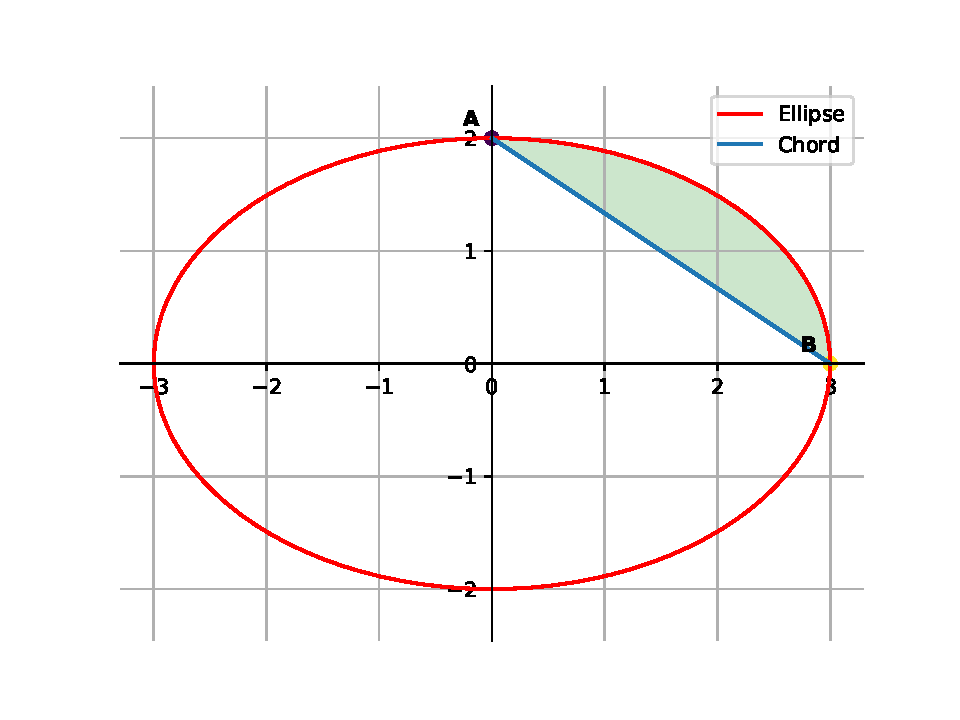
\includegraphics[width=0.75\columnwidth]{chapters/11/10/1/14/figs/fig.pdf}
\caption{}
\label{fig:chapters/11/10/1/14/1}
\end{figure}
\solution
\begin{enumerate}[label=\thesection.\arabic*.,ref=\thesection.\theenumi]
\numberwithin{equation}{enumi}
\item The equation of a line is given by 
\begin{align}
			\label{eq:app-line-school}
	y &= mx + c
	\\
	\implies \myvec{x \\ y} &= \myvec{x \\ 
	 mx + c} =\myvec{0 \\ c} + x\myvec{1 \\ m}
\end{align}
			yielding \eqref{eq:geo-param}.
\item 			\eqref{eq:app-line-school} can also be expressed as
\begin{align}
	y - mx &= c 
	\\
	\implies \myvec{-m & 1}\myvec{x \\ y} &= c
\end{align}
			yielding \eqref{eq:geo-normal}.
		\item The direction vector is 
\begin{align}
			\label{eq:app-line-school-dir}
\vec{m} = \myvec{1 \\ m}
\end{align}
and the normal vector is
\begin{align}
\vec{n}=\myvec{-m \\ 1}
			\label{eq:app-line-school-normal}
\end{align}
  \item From \eqref{eq:geo-param}, 
	  if $\vec{A},\vec{D}$ and $\vec{C}$ are on the same line,
		\label{prop:app-lin-dep}
\begin{align}
			\vec{D}=\vec{A}+q\vec{m} 
			\\ 
			\vec{C}=\vec{D}+p\vec{m} \\
			\label{eq:app-collinear} 
			\implies 	p\brak{\vec{D}-\vec{A}} 
			+ q\brak{\vec{D}-\vec{C}} = 0, \quad p, q \ne 0 \\ 
			\implies \vec{D} = \frac{p\vec{A}+q\vec{C}}{p+q} 
			\end{align} 
			yielding \eqref{eq:section_formula} upon substituting \begin{align} k = \frac{p}{q}. \end{align} 
			$\brak{\vec{D}-\vec{A}}, \brak{\vec{D}-\vec{C}}$ 
		are then said to be {\em linearly dependent}.
	\item If $\vec{A}, \vec{B}, \vec{C}$ are collinear,  from \eqref{eq:geo-normal}, \begin{align}
	 \vec{n}^{\top}\vec{A} &=  c 
	 \\
	 \vec{n}^{\top}\vec{B} &=  c 
	 \\
	 \vec{n}^{\top}\vec{C} &=  c 
\end{align}
which can be expressed as 
\begin{align}
		\label{prop:app-lin-eq}
	\myvec{ \vec{A} & \vec{B} & \vec{C}}^{\top}\vec{n} = c\myvec{1 \\ 1 \\ 1}
	\\
	\equiv \myvec{ \vec{A} & \vec{B} & \vec{C}}^{\top}\vec{n} = \myvec{1 \\ 1 \\ 1}
		\label{prop:app-lin-eq-unit-mat},
	\\
	\implies 
	\myvec{ \vec{A} & \vec{B} & \vec{C}\\ 1 & 1 &1 }^{\top}\myvec{\vec{n} \\ -1} &= \vec{0}
		\label{prop:app-lin-dep-rank}
\end{align}
yielding
		\begin{align}
			\label{eq:app-line-rank-2}
			\rank{\myvec{1 & 1 & 1 \\ \vec{A}& \vec{B}&\vec{C}}} = 2
		\end{align}
			  Rank is defined to be the number of linearly indpendent rows or columns of a matrix.
		\item
The equation of a line can also be expressed as
\begin{align}
	 \vec{n}^{\top}\vec{x} &=   1
		\label{prop:app-lin-eq-unit}
\end{align}
	  \end{enumerate}

\item Slope of a line which cuts off intercepts of equal length on the axes is 
	\rule{1cm}{0.1pt}.
\item If the coordinates of middle point of the portion of a line intercepted between the coordinate axes is (3, 2), then the equation of the line will be
\rule{1cm}{0.1pt}.
\item If the line $\frac{x}{a}+\frac{y}{b}=1$ passes the points (2, -3) and (4, -5),  then $(a, b)$ is 
\rule{1cm}{0.1pt}.
\item The intercepts made by the plane $2x-3y+5z+4=0$ on the co-ordinate axis are $\brak{-2, \frac{4}{3}, -\frac{4}{5}}$.
\item The line $\overrightarrow{r}=2\hat{i}-3\hat{j}-\hat{k}+\lambda(\hat{i}-\hat{j}+2\hat{k})$ lies in the plane $\overrightarrow{r} \cdot (3\hat{i}+\hat{j}-\hat{k})+2=0$.
\item Find the equation of the line joining $(1, 2)$ and $(3, 6)$.
\item Find the equation of the line joining $(3, 1)$ and $(9, 3)$.
\item If the point (3,  4) lies on the line $3y=ax+7$,  find the value of $a$.
\item  Find the equation of the line that passes through the point with position vector $2\hat{i}-\hat{j}+4\hat{k}$ and is in direction $\hat{i}+2\hat{j}-\hat{k}$.
\item The cartesian equation of a line is $ \frac{x-5}{3}=\frac{y+4}{7}=\frac{z-6}{2}$. Write its vector form.
\item Find the equation of the line that passes through the origin and $(5, -2, 3)$.
\item Find the equation of the line that passes through the points $(3, -2, -5), (3, -2, 6)$.
\item Find the coordinates of the point where the line through $(5,1,6)$ and $(3,4,1)$ crosses the $YZ$-plane.
\item Find the coordinates of the point where the line through $(5,1,6)$ and $(3,4,1)$ crosses the $ZX$-plane.
\item Find the coordinates of the point where the line through $(3,-4,-5)$ and $(2,-3,1)$ crosses the plane $2x+y+x=7$.
\item Find the equation of the line through $(-2,3)$ with slope $-4$
\item Write the equation of the line through the points $(1,-1)$ and $(3,5)$.
\item Write the equation of the lines for which $\tan \theta=\frac{1}{2}$, where $\theta$ is the inclination of the line and
\begin{enumerate}
\item  y-intercept is $\frac{-3}{2}$ 
\item  x-intercept is $4$.
\end{enumerate}
\item Find the equation of the lines which makes intercepts $-3$ and $2$ on the x- and y-axes respectively.
\item Equation of a line is $3x-4y+10=0$, find its
\begin{enumerate}
\item  Slope
\item  x and y-intercepts.
\end{enumerate}
\item Determine the ratio in which the line $2x+y  - 4=0$ divides the line segment joining the points  $\vec{A}(2, - 2)$  and  $\vec{B}(3, 7)$.
\\
\solution
	\begin{enumerate}[label=\thesubsection.\arabic*,ref=\thesubsection.\theenumi]
\item Find the coordinates of the point which divides the join of $(-1,7) $ and $ (4,-3)$ in the ratio 2:3.
	\\
		\solution
	\begin{enumerate}[label=\thesubsection.\arabic*,ref=\thesubsection.\theenumi]
\item Find the coordinates of the point which divides the join of $(-1,7) $ and $ (4,-3)$ in the ratio 2:3.
	\\
		\solution
	\begin{enumerate}[label=\thesubsection.\arabic*,ref=\thesubsection.\theenumi]
\item Find the coordinates of the point which divides the join of $(-1,7) $ and $ (4,-3)$ in the ratio 2:3.
	\\
		\solution
	\input{chapters/10/7/2/1/section.tex}
\item Find the coordinates of the point $\vec{R}$ on the line segment joining the points $\vec{P}(-1,3)$ and $\vec{Q}(2,5)$ such that $PR=\frac{3}{5}PQ$.
\item Find the ratio in which the point $\vec{P}\brak{\frac{3}{4},\frac{5}{12}}$ divides the line segment joining the points $\vec{A}\brak{\frac{1}{2},\frac{3}{2}}$ and $ \vec{B}(2,-5)$.
\item Find the coordinates of the point which divides the line segment joining the points $(4,-3)$ and $(8,5)$ in the ratio $3:1$ internally.
\item Find the coordinates of the point $\vec{P}$ on $AD$ such that $AP : PD = 2 : 1$.
\item If the point $\vec{P} (2, 1)$ lies on the line segment joining points $\vec{A} (4, 2)$  and $ \vec{B} (8, 4)$,
then
\begin{enumerate}
	\item $AP =\frac{1}{3}{AB}$ 
\item ${AP}={PE}$
\item ${PB}=\frac{1}{3}{AB}$
\item${AP}=\frac{1}{2}{AB}$
 \end{enumerate}
\item Find the ratio in which the line segment joining the points $(-3,10)$  and  $(6,-8)$  is divided by $ (-1,6)$.
	\\
		\solution
	\input{chapters/10/7/2/4/section.tex}
\item Find the position vector of the mid point of the vector joining the points $\vec{P}$(2, 3, 4)
and $\vec{Q}$(4, 1, –2).
\\
\solution
		\input{chapters/12/10/2/16/section.tex}
\item Let $\vec{A}(4, 2), \vec{B}(6, 5)$  and $ \vec{C}(1, 4)$ be the vertices of $\triangle ABC$.
\begin{enumerate}
\item If $\vec{A}$ and  $\vec{B}$ are $(-2,-2)$ and  $(2,-4)$, respectively, find the coordinates of $\vec{P}$ such that $AP= \frac {3}{7}AB$  and $ \vec{P}$ lies on the line segment $AB$.
	\\
		\solution
	\input{chapters/10/7/2/8/section.tex}
\item Find the coordinates of the points which divide the line segment joining $A(-2,2)$  and  $\vec{B}(2,8)$ into four equal parts.
	\\
		\solution
	\input{chapters/10/7/2/9/section.tex}
\item In what ratio does the point $(-4,6)$ divide the line segment joining the points $\vec{A}(-6,0)$ and $\vec{B}(3,-8)$?
\item Given that $\vec{P}(3,2,-4), \vec{Q}(5,4,-6)$ and $\vec{R}(9,8,-10)$ are collinear. Find the ratio in which $\vec{Q}$ divides $PR$.
\item Points $\vec{A}(-6,10),\vec{B}(-4,6)$  and  $\vec{C}(3,-8)$ are collinear such that $AB=  \frac{2}{9}AC$.
\item The point which divides the line segment joining the points $\vec{P} (7, –6) $  and  $\vec{Q}(3, 4)$ in the 
ratio 1 : 2 internally lies in  which quadrant?
\item Find the coordinates of the points of trisection of the line segment joining $(4,-1)$  and  $(-2,3)$.
	\\
		\solution
	\input{chapters/10/7/2/2/section.tex}
\item Find the coordinates of the points which trisect the line segment joining the points $\vec{P}(4,2,-6)$ and $\vec{Q}(10,-16,6)$.
\item Find the coordinates of the points of trisection (i.e. points dividing to three equal parts) of the line segment joining the points $\vec{A}(2,-2)$ and $\vec{B}(-7,4)$.
\item Point $\vec{P}(5,-3)$ is one of the two points of trisection of line segment joining the points $\vec{A}(7,-2)$ and $\vec{B}(1,-5)$
\item Find the position vector of a point $\vec{R}$ which divides the line joining two points $\vec{P}$
and $\vec{Q}$ whose position vectors are $\hat{i}+2\hat{j}-\hat{k}$ and $-\hat{i}+\hat{j}+\hat{k}$ respectively, in the
ratio 2 : 1
\begin{enumerate}
    \item  internally
    \item  externally
\end{enumerate}
%\solution
%		\input{chapters/12/10/2/15/section.tex}
\item Find the coordinates of the point which divides the line segment joining the points which divides the line segment joining  the points $(-2,3,5)$ and $(1,-4,6)$ in the ratio 
\begin{enumerate}
\item $2:3$ internally,
\item $2:3$ externally
\end{enumerate}
\item Find the coordinates of the point which divides the line segment joining the points $(1,-2,3)$ and $(3,4,-5)$ in the ratio $2:3$
\begin{enumerate}
\item internally, and
\item externally
\end{enumerate}
\item Consider two points $\vec{P}$ and $\vec{Q}$ with position vectors $\overrightarrow{OP} = 3\overrightarrow{a}-2\overrightarrow{b}$ and $\overrightarrow{OQ}=\overrightarrow{a}+\overrightarrow{b}$. Find the position vector of a point $\vec{R}$ which divides the line joining $\vec{P}$ and $\vec{Q}$ in the ratio $2:1$, 
\begin{enumerate}
\item internally, and 
\item externally.
\end{enumerate}
\item The median from $\vec{A}$ meets $BC$ at $\vec{D}$. Find the coordinates of the point $\vec{D}$.
\item Find the coordinates of points $\vec{Q}$ and $\vec{R}$ on medians $BE$ and $CF$ respectively such that $BQ : QE = 2 : 1$  and  $CR : RF = 2 : 1$.
\item What do you observe?
\item If $\vec{A}, \vec{B}$ and $\vec{C}$  are the vertices of $\triangle ABC$, find the coordinates of the centroid of the triangle.
\end{enumerate}
\solution
	\input{chapters/10/7/4/7/section.tex}
\item If $\vec{P}(9a-2,-b)$ divides line segment joining $\vec{A}(3a+1,-3)$ and $\vec{B}(8a,5)$ in the ratio 3:1, find the values of $a$ and $b$.
\item Find the position vector of a point $\vec{R}$ which divides the line joining two points $\vec{P}$ and $\vec{Q}$ whose position vectors are $2\vec{a}+\vec{b}$ and $\vec{a}-3\vec{b}$ externally in the ratio $1:2$.
\item The position vector of the point which divides the join of points 2$\vec{a}$-3$\vec{b}$ $\text{and}$ $\vec{a}+\vec{b}$ in the ratio 3:1 is \rule{1cm}{0.1pt}.
\item If $\vec{a}$ and $\vec{b}$ are the postion vectors of $\vec{A}$ and $\vec{B}$, respectively, find the position vector of a point $\vec{C}$ in $BA$ produced such that $BC=1.5BA$.
\item Find the position vector of a point $\vec{R}$ which divides the line joining two points $\vec{P}$ and $\vec{Q}$ whose position vectors are $(2\vec{a}+\vec{b})$ and $(\vec{a}-3\vec{b})$
externally in the ratio 1 : 2. Also, show that $\vec{P}$ is the mid point of the line segment $RQ$.
\end{enumerate}

\item Find the coordinates of the point $\vec{R}$ on the line segment joining the points $\vec{P}(-1,3)$ and $\vec{Q}(2,5)$ such that $PR=\frac{3}{5}PQ$.
\item Find the ratio in which the point $\vec{P}\brak{\frac{3}{4},\frac{5}{12}}$ divides the line segment joining the points $\vec{A}\brak{\frac{1}{2},\frac{3}{2}}$ and $ \vec{B}(2,-5)$.
\item Find the coordinates of the point which divides the line segment joining the points $(4,-3)$ and $(8,5)$ in the ratio $3:1$ internally.
\item Find the coordinates of the point $\vec{P}$ on $AD$ such that $AP : PD = 2 : 1$.
\item If the point $\vec{P} (2, 1)$ lies on the line segment joining points $\vec{A} (4, 2)$  and $ \vec{B} (8, 4)$,
then
\begin{enumerate}
	\item $AP =\frac{1}{3}{AB}$ 
\item ${AP}={PE}$
\item ${PB}=\frac{1}{3}{AB}$
\item${AP}=\frac{1}{2}{AB}$
 \end{enumerate}
\item Find the ratio in which the line segment joining the points $(-3,10)$  and  $(6,-8)$  is divided by $ (-1,6)$.
	\\
		\solution
	\iffalse
Using section formula,
\begin{align}
         \myvec{-1\\6} &=\frac{{\myvec{-3\\10}+k\myvec{6\\-8}}}{1+k}\\
	 \implies 7k\myvec{1 \\ -2} &= 2\myvec{1 \\ -2}
	 \\
	 \text{or, } k &= \frac{2}{7}.
\end{align}
\fi
In 
			\eqref{eq:section_formula-k}, substituting
			\begin{align}
				\vec{B} &= \myvec{-3\\10}, \vec{C} = \myvec{6\\-8}, \vec{D} = \myvec{-1\\6},
				\\
				k &= \frac{\myvec{-2 & 4}\myvec{-7 \\ 14}}{\norm{\myvec{-7 \\ 14}}^2} = \frac{2}{7}
			\end{align}
\iffalse
See \figref{fig:10/7/2/4Fig1}.
\begin{figure}[H]
 \begin{center}
  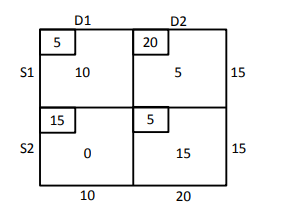
\includegraphics[width=0.75\columnwidth]{chapters/10/7/2/4/figs/fig.png}
 \end{center}
\caption{}
\label{fig:10/7/2/4Fig1}
\end{figure}
\fi

\item Find the position vector of the mid point of the vector joining the points $\vec{P}$(2, 3, 4)
and $\vec{Q}$(4, 1, –2).
\\
\solution
		\begin{enumerate}[label=\thesubsection.\arabic*,ref=\thesubsection.\theenumi]
\item Find the coordinates of the point which divides the join of $(-1,7) $ and $ (4,-3)$ in the ratio 2:3.
	\\
		\solution
	\input{chapters/10/7/2/1/section.tex}
\item Find the coordinates of the point $\vec{R}$ on the line segment joining the points $\vec{P}(-1,3)$ and $\vec{Q}(2,5)$ such that $PR=\frac{3}{5}PQ$.
\item Find the ratio in which the point $\vec{P}\brak{\frac{3}{4},\frac{5}{12}}$ divides the line segment joining the points $\vec{A}\brak{\frac{1}{2},\frac{3}{2}}$ and $ \vec{B}(2,-5)$.
\item Find the coordinates of the point which divides the line segment joining the points $(4,-3)$ and $(8,5)$ in the ratio $3:1$ internally.
\item Find the coordinates of the point $\vec{P}$ on $AD$ such that $AP : PD = 2 : 1$.
\item If the point $\vec{P} (2, 1)$ lies on the line segment joining points $\vec{A} (4, 2)$  and $ \vec{B} (8, 4)$,
then
\begin{enumerate}
	\item $AP =\frac{1}{3}{AB}$ 
\item ${AP}={PE}$
\item ${PB}=\frac{1}{3}{AB}$
\item${AP}=\frac{1}{2}{AB}$
 \end{enumerate}
\item Find the ratio in which the line segment joining the points $(-3,10)$  and  $(6,-8)$  is divided by $ (-1,6)$.
	\\
		\solution
	\input{chapters/10/7/2/4/section.tex}
\item Find the position vector of the mid point of the vector joining the points $\vec{P}$(2, 3, 4)
and $\vec{Q}$(4, 1, –2).
\\
\solution
		\input{chapters/12/10/2/16/section.tex}
\item Let $\vec{A}(4, 2), \vec{B}(6, 5)$  and $ \vec{C}(1, 4)$ be the vertices of $\triangle ABC$.
\begin{enumerate}
\item If $\vec{A}$ and  $\vec{B}$ are $(-2,-2)$ and  $(2,-4)$, respectively, find the coordinates of $\vec{P}$ such that $AP= \frac {3}{7}AB$  and $ \vec{P}$ lies on the line segment $AB$.
	\\
		\solution
	\input{chapters/10/7/2/8/section.tex}
\item Find the coordinates of the points which divide the line segment joining $A(-2,2)$  and  $\vec{B}(2,8)$ into four equal parts.
	\\
		\solution
	\input{chapters/10/7/2/9/section.tex}
\item In what ratio does the point $(-4,6)$ divide the line segment joining the points $\vec{A}(-6,0)$ and $\vec{B}(3,-8)$?
\item Given that $\vec{P}(3,2,-4), \vec{Q}(5,4,-6)$ and $\vec{R}(9,8,-10)$ are collinear. Find the ratio in which $\vec{Q}$ divides $PR$.
\item Points $\vec{A}(-6,10),\vec{B}(-4,6)$  and  $\vec{C}(3,-8)$ are collinear such that $AB=  \frac{2}{9}AC$.
\item The point which divides the line segment joining the points $\vec{P} (7, –6) $  and  $\vec{Q}(3, 4)$ in the 
ratio 1 : 2 internally lies in  which quadrant?
\item Find the coordinates of the points of trisection of the line segment joining $(4,-1)$  and  $(-2,3)$.
	\\
		\solution
	\input{chapters/10/7/2/2/section.tex}
\item Find the coordinates of the points which trisect the line segment joining the points $\vec{P}(4,2,-6)$ and $\vec{Q}(10,-16,6)$.
\item Find the coordinates of the points of trisection (i.e. points dividing to three equal parts) of the line segment joining the points $\vec{A}(2,-2)$ and $\vec{B}(-7,4)$.
\item Point $\vec{P}(5,-3)$ is one of the two points of trisection of line segment joining the points $\vec{A}(7,-2)$ and $\vec{B}(1,-5)$
\item Find the position vector of a point $\vec{R}$ which divides the line joining two points $\vec{P}$
and $\vec{Q}$ whose position vectors are $\hat{i}+2\hat{j}-\hat{k}$ and $-\hat{i}+\hat{j}+\hat{k}$ respectively, in the
ratio 2 : 1
\begin{enumerate}
    \item  internally
    \item  externally
\end{enumerate}
%\solution
%		\input{chapters/12/10/2/15/section.tex}
\item Find the coordinates of the point which divides the line segment joining the points which divides the line segment joining  the points $(-2,3,5)$ and $(1,-4,6)$ in the ratio 
\begin{enumerate}
\item $2:3$ internally,
\item $2:3$ externally
\end{enumerate}
\item Find the coordinates of the point which divides the line segment joining the points $(1,-2,3)$ and $(3,4,-5)$ in the ratio $2:3$
\begin{enumerate}
\item internally, and
\item externally
\end{enumerate}
\item Consider two points $\vec{P}$ and $\vec{Q}$ with position vectors $\overrightarrow{OP} = 3\overrightarrow{a}-2\overrightarrow{b}$ and $\overrightarrow{OQ}=\overrightarrow{a}+\overrightarrow{b}$. Find the position vector of a point $\vec{R}$ which divides the line joining $\vec{P}$ and $\vec{Q}$ in the ratio $2:1$, 
\begin{enumerate}
\item internally, and 
\item externally.
\end{enumerate}
\item The median from $\vec{A}$ meets $BC$ at $\vec{D}$. Find the coordinates of the point $\vec{D}$.
\item Find the coordinates of points $\vec{Q}$ and $\vec{R}$ on medians $BE$ and $CF$ respectively such that $BQ : QE = 2 : 1$  and  $CR : RF = 2 : 1$.
\item What do you observe?
\item If $\vec{A}, \vec{B}$ and $\vec{C}$  are the vertices of $\triangle ABC$, find the coordinates of the centroid of the triangle.
\end{enumerate}
\solution
	\input{chapters/10/7/4/7/section.tex}
\item If $\vec{P}(9a-2,-b)$ divides line segment joining $\vec{A}(3a+1,-3)$ and $\vec{B}(8a,5)$ in the ratio 3:1, find the values of $a$ and $b$.
\item Find the position vector of a point $\vec{R}$ which divides the line joining two points $\vec{P}$ and $\vec{Q}$ whose position vectors are $2\vec{a}+\vec{b}$ and $\vec{a}-3\vec{b}$ externally in the ratio $1:2$.
\item The position vector of the point which divides the join of points 2$\vec{a}$-3$\vec{b}$ $\text{and}$ $\vec{a}+\vec{b}$ in the ratio 3:1 is \rule{1cm}{0.1pt}.
\item If $\vec{a}$ and $\vec{b}$ are the postion vectors of $\vec{A}$ and $\vec{B}$, respectively, find the position vector of a point $\vec{C}$ in $BA$ produced such that $BC=1.5BA$.
\item Find the position vector of a point $\vec{R}$ which divides the line joining two points $\vec{P}$ and $\vec{Q}$ whose position vectors are $(2\vec{a}+\vec{b})$ and $(\vec{a}-3\vec{b})$
externally in the ratio 1 : 2. Also, show that $\vec{P}$ is the mid point of the line segment $RQ$.
\end{enumerate}

\item Let $\vec{A}(4, 2), \vec{B}(6, 5)$  and $ \vec{C}(1, 4)$ be the vertices of $\triangle ABC$.
\begin{enumerate}
\item If $\vec{A}$ and  $\vec{B}$ are $(-2,-2)$ and  $(2,-4)$, respectively, find the coordinates of $\vec{P}$ such that $AP= \frac {3}{7}AB$  and $ \vec{P}$ lies on the line segment $AB$.
	\\
		\solution
	\begin{enumerate}[label=\thesubsection.\arabic*,ref=\thesubsection.\theenumi]
\item Find the coordinates of the point which divides the join of $(-1,7) $ and $ (4,-3)$ in the ratio 2:3.
	\\
		\solution
	\input{chapters/10/7/2/1/section.tex}
\item Find the coordinates of the point $\vec{R}$ on the line segment joining the points $\vec{P}(-1,3)$ and $\vec{Q}(2,5)$ such that $PR=\frac{3}{5}PQ$.
\item Find the ratio in which the point $\vec{P}\brak{\frac{3}{4},\frac{5}{12}}$ divides the line segment joining the points $\vec{A}\brak{\frac{1}{2},\frac{3}{2}}$ and $ \vec{B}(2,-5)$.
\item Find the coordinates of the point which divides the line segment joining the points $(4,-3)$ and $(8,5)$ in the ratio $3:1$ internally.
\item Find the coordinates of the point $\vec{P}$ on $AD$ such that $AP : PD = 2 : 1$.
\item If the point $\vec{P} (2, 1)$ lies on the line segment joining points $\vec{A} (4, 2)$  and $ \vec{B} (8, 4)$,
then
\begin{enumerate}
	\item $AP =\frac{1}{3}{AB}$ 
\item ${AP}={PE}$
\item ${PB}=\frac{1}{3}{AB}$
\item${AP}=\frac{1}{2}{AB}$
 \end{enumerate}
\item Find the ratio in which the line segment joining the points $(-3,10)$  and  $(6,-8)$  is divided by $ (-1,6)$.
	\\
		\solution
	\input{chapters/10/7/2/4/section.tex}
\item Find the position vector of the mid point of the vector joining the points $\vec{P}$(2, 3, 4)
and $\vec{Q}$(4, 1, –2).
\\
\solution
		\input{chapters/12/10/2/16/section.tex}
\item Let $\vec{A}(4, 2), \vec{B}(6, 5)$  and $ \vec{C}(1, 4)$ be the vertices of $\triangle ABC$.
\begin{enumerate}
\item If $\vec{A}$ and  $\vec{B}$ are $(-2,-2)$ and  $(2,-4)$, respectively, find the coordinates of $\vec{P}$ such that $AP= \frac {3}{7}AB$  and $ \vec{P}$ lies on the line segment $AB$.
	\\
		\solution
	\input{chapters/10/7/2/8/section.tex}
\item Find the coordinates of the points which divide the line segment joining $A(-2,2)$  and  $\vec{B}(2,8)$ into four equal parts.
	\\
		\solution
	\input{chapters/10/7/2/9/section.tex}
\item In what ratio does the point $(-4,6)$ divide the line segment joining the points $\vec{A}(-6,0)$ and $\vec{B}(3,-8)$?
\item Given that $\vec{P}(3,2,-4), \vec{Q}(5,4,-6)$ and $\vec{R}(9,8,-10)$ are collinear. Find the ratio in which $\vec{Q}$ divides $PR$.
\item Points $\vec{A}(-6,10),\vec{B}(-4,6)$  and  $\vec{C}(3,-8)$ are collinear such that $AB=  \frac{2}{9}AC$.
\item The point which divides the line segment joining the points $\vec{P} (7, –6) $  and  $\vec{Q}(3, 4)$ in the 
ratio 1 : 2 internally lies in  which quadrant?
\item Find the coordinates of the points of trisection of the line segment joining $(4,-1)$  and  $(-2,3)$.
	\\
		\solution
	\input{chapters/10/7/2/2/section.tex}
\item Find the coordinates of the points which trisect the line segment joining the points $\vec{P}(4,2,-6)$ and $\vec{Q}(10,-16,6)$.
\item Find the coordinates of the points of trisection (i.e. points dividing to three equal parts) of the line segment joining the points $\vec{A}(2,-2)$ and $\vec{B}(-7,4)$.
\item Point $\vec{P}(5,-3)$ is one of the two points of trisection of line segment joining the points $\vec{A}(7,-2)$ and $\vec{B}(1,-5)$
\item Find the position vector of a point $\vec{R}$ which divides the line joining two points $\vec{P}$
and $\vec{Q}$ whose position vectors are $\hat{i}+2\hat{j}-\hat{k}$ and $-\hat{i}+\hat{j}+\hat{k}$ respectively, in the
ratio 2 : 1
\begin{enumerate}
    \item  internally
    \item  externally
\end{enumerate}
%\solution
%		\input{chapters/12/10/2/15/section.tex}
\item Find the coordinates of the point which divides the line segment joining the points which divides the line segment joining  the points $(-2,3,5)$ and $(1,-4,6)$ in the ratio 
\begin{enumerate}
\item $2:3$ internally,
\item $2:3$ externally
\end{enumerate}
\item Find the coordinates of the point which divides the line segment joining the points $(1,-2,3)$ and $(3,4,-5)$ in the ratio $2:3$
\begin{enumerate}
\item internally, and
\item externally
\end{enumerate}
\item Consider two points $\vec{P}$ and $\vec{Q}$ with position vectors $\overrightarrow{OP} = 3\overrightarrow{a}-2\overrightarrow{b}$ and $\overrightarrow{OQ}=\overrightarrow{a}+\overrightarrow{b}$. Find the position vector of a point $\vec{R}$ which divides the line joining $\vec{P}$ and $\vec{Q}$ in the ratio $2:1$, 
\begin{enumerate}
\item internally, and 
\item externally.
\end{enumerate}
\item The median from $\vec{A}$ meets $BC$ at $\vec{D}$. Find the coordinates of the point $\vec{D}$.
\item Find the coordinates of points $\vec{Q}$ and $\vec{R}$ on medians $BE$ and $CF$ respectively such that $BQ : QE = 2 : 1$  and  $CR : RF = 2 : 1$.
\item What do you observe?
\item If $\vec{A}, \vec{B}$ and $\vec{C}$  are the vertices of $\triangle ABC$, find the coordinates of the centroid of the triangle.
\end{enumerate}
\solution
	\input{chapters/10/7/4/7/section.tex}
\item If $\vec{P}(9a-2,-b)$ divides line segment joining $\vec{A}(3a+1,-3)$ and $\vec{B}(8a,5)$ in the ratio 3:1, find the values of $a$ and $b$.
\item Find the position vector of a point $\vec{R}$ which divides the line joining two points $\vec{P}$ and $\vec{Q}$ whose position vectors are $2\vec{a}+\vec{b}$ and $\vec{a}-3\vec{b}$ externally in the ratio $1:2$.
\item The position vector of the point which divides the join of points 2$\vec{a}$-3$\vec{b}$ $\text{and}$ $\vec{a}+\vec{b}$ in the ratio 3:1 is \rule{1cm}{0.1pt}.
\item If $\vec{a}$ and $\vec{b}$ are the postion vectors of $\vec{A}$ and $\vec{B}$, respectively, find the position vector of a point $\vec{C}$ in $BA$ produced such that $BC=1.5BA$.
\item Find the position vector of a point $\vec{R}$ which divides the line joining two points $\vec{P}$ and $\vec{Q}$ whose position vectors are $(2\vec{a}+\vec{b})$ and $(\vec{a}-3\vec{b})$
externally in the ratio 1 : 2. Also, show that $\vec{P}$ is the mid point of the line segment $RQ$.
\end{enumerate}

\item Find the coordinates of the points which divide the line segment joining $A(-2,2)$  and  $\vec{B}(2,8)$ into four equal parts.
	\\
		\solution
	\begin{enumerate}[label=\thesubsection.\arabic*,ref=\thesubsection.\theenumi]
\item Find the coordinates of the point which divides the join of $(-1,7) $ and $ (4,-3)$ in the ratio 2:3.
	\\
		\solution
	\input{chapters/10/7/2/1/section.tex}
\item Find the coordinates of the point $\vec{R}$ on the line segment joining the points $\vec{P}(-1,3)$ and $\vec{Q}(2,5)$ such that $PR=\frac{3}{5}PQ$.
\item Find the ratio in which the point $\vec{P}\brak{\frac{3}{4},\frac{5}{12}}$ divides the line segment joining the points $\vec{A}\brak{\frac{1}{2},\frac{3}{2}}$ and $ \vec{B}(2,-5)$.
\item Find the coordinates of the point which divides the line segment joining the points $(4,-3)$ and $(8,5)$ in the ratio $3:1$ internally.
\item Find the coordinates of the point $\vec{P}$ on $AD$ such that $AP : PD = 2 : 1$.
\item If the point $\vec{P} (2, 1)$ lies on the line segment joining points $\vec{A} (4, 2)$  and $ \vec{B} (8, 4)$,
then
\begin{enumerate}
	\item $AP =\frac{1}{3}{AB}$ 
\item ${AP}={PE}$
\item ${PB}=\frac{1}{3}{AB}$
\item${AP}=\frac{1}{2}{AB}$
 \end{enumerate}
\item Find the ratio in which the line segment joining the points $(-3,10)$  and  $(6,-8)$  is divided by $ (-1,6)$.
	\\
		\solution
	\input{chapters/10/7/2/4/section.tex}
\item Find the position vector of the mid point of the vector joining the points $\vec{P}$(2, 3, 4)
and $\vec{Q}$(4, 1, –2).
\\
\solution
		\input{chapters/12/10/2/16/section.tex}
\item Let $\vec{A}(4, 2), \vec{B}(6, 5)$  and $ \vec{C}(1, 4)$ be the vertices of $\triangle ABC$.
\begin{enumerate}
\item If $\vec{A}$ and  $\vec{B}$ are $(-2,-2)$ and  $(2,-4)$, respectively, find the coordinates of $\vec{P}$ such that $AP= \frac {3}{7}AB$  and $ \vec{P}$ lies on the line segment $AB$.
	\\
		\solution
	\input{chapters/10/7/2/8/section.tex}
\item Find the coordinates of the points which divide the line segment joining $A(-2,2)$  and  $\vec{B}(2,8)$ into four equal parts.
	\\
		\solution
	\input{chapters/10/7/2/9/section.tex}
\item In what ratio does the point $(-4,6)$ divide the line segment joining the points $\vec{A}(-6,0)$ and $\vec{B}(3,-8)$?
\item Given that $\vec{P}(3,2,-4), \vec{Q}(5,4,-6)$ and $\vec{R}(9,8,-10)$ are collinear. Find the ratio in which $\vec{Q}$ divides $PR$.
\item Points $\vec{A}(-6,10),\vec{B}(-4,6)$  and  $\vec{C}(3,-8)$ are collinear such that $AB=  \frac{2}{9}AC$.
\item The point which divides the line segment joining the points $\vec{P} (7, –6) $  and  $\vec{Q}(3, 4)$ in the 
ratio 1 : 2 internally lies in  which quadrant?
\item Find the coordinates of the points of trisection of the line segment joining $(4,-1)$  and  $(-2,3)$.
	\\
		\solution
	\input{chapters/10/7/2/2/section.tex}
\item Find the coordinates of the points which trisect the line segment joining the points $\vec{P}(4,2,-6)$ and $\vec{Q}(10,-16,6)$.
\item Find the coordinates of the points of trisection (i.e. points dividing to three equal parts) of the line segment joining the points $\vec{A}(2,-2)$ and $\vec{B}(-7,4)$.
\item Point $\vec{P}(5,-3)$ is one of the two points of trisection of line segment joining the points $\vec{A}(7,-2)$ and $\vec{B}(1,-5)$
\item Find the position vector of a point $\vec{R}$ which divides the line joining two points $\vec{P}$
and $\vec{Q}$ whose position vectors are $\hat{i}+2\hat{j}-\hat{k}$ and $-\hat{i}+\hat{j}+\hat{k}$ respectively, in the
ratio 2 : 1
\begin{enumerate}
    \item  internally
    \item  externally
\end{enumerate}
%\solution
%		\input{chapters/12/10/2/15/section.tex}
\item Find the coordinates of the point which divides the line segment joining the points which divides the line segment joining  the points $(-2,3,5)$ and $(1,-4,6)$ in the ratio 
\begin{enumerate}
\item $2:3$ internally,
\item $2:3$ externally
\end{enumerate}
\item Find the coordinates of the point which divides the line segment joining the points $(1,-2,3)$ and $(3,4,-5)$ in the ratio $2:3$
\begin{enumerate}
\item internally, and
\item externally
\end{enumerate}
\item Consider two points $\vec{P}$ and $\vec{Q}$ with position vectors $\overrightarrow{OP} = 3\overrightarrow{a}-2\overrightarrow{b}$ and $\overrightarrow{OQ}=\overrightarrow{a}+\overrightarrow{b}$. Find the position vector of a point $\vec{R}$ which divides the line joining $\vec{P}$ and $\vec{Q}$ in the ratio $2:1$, 
\begin{enumerate}
\item internally, and 
\item externally.
\end{enumerate}
\item The median from $\vec{A}$ meets $BC$ at $\vec{D}$. Find the coordinates of the point $\vec{D}$.
\item Find the coordinates of points $\vec{Q}$ and $\vec{R}$ on medians $BE$ and $CF$ respectively such that $BQ : QE = 2 : 1$  and  $CR : RF = 2 : 1$.
\item What do you observe?
\item If $\vec{A}, \vec{B}$ and $\vec{C}$  are the vertices of $\triangle ABC$, find the coordinates of the centroid of the triangle.
\end{enumerate}
\solution
	\input{chapters/10/7/4/7/section.tex}
\item If $\vec{P}(9a-2,-b)$ divides line segment joining $\vec{A}(3a+1,-3)$ and $\vec{B}(8a,5)$ in the ratio 3:1, find the values of $a$ and $b$.
\item Find the position vector of a point $\vec{R}$ which divides the line joining two points $\vec{P}$ and $\vec{Q}$ whose position vectors are $2\vec{a}+\vec{b}$ and $\vec{a}-3\vec{b}$ externally in the ratio $1:2$.
\item The position vector of the point which divides the join of points 2$\vec{a}$-3$\vec{b}$ $\text{and}$ $\vec{a}+\vec{b}$ in the ratio 3:1 is \rule{1cm}{0.1pt}.
\item If $\vec{a}$ and $\vec{b}$ are the postion vectors of $\vec{A}$ and $\vec{B}$, respectively, find the position vector of a point $\vec{C}$ in $BA$ produced such that $BC=1.5BA$.
\item Find the position vector of a point $\vec{R}$ which divides the line joining two points $\vec{P}$ and $\vec{Q}$ whose position vectors are $(2\vec{a}+\vec{b})$ and $(\vec{a}-3\vec{b})$
externally in the ratio 1 : 2. Also, show that $\vec{P}$ is the mid point of the line segment $RQ$.
\end{enumerate}

\item In what ratio does the point $(-4,6)$ divide the line segment joining the points $\vec{A}(-6,0)$ and $\vec{B}(3,-8)$?
\item Given that $\vec{P}(3,2,-4), \vec{Q}(5,4,-6)$ and $\vec{R}(9,8,-10)$ are collinear. Find the ratio in which $\vec{Q}$ divides $PR$.
\item Points $\vec{A}(-6,10),\vec{B}(-4,6)$  and  $\vec{C}(3,-8)$ are collinear such that $AB=  \frac{2}{9}AC$.
\item The point which divides the line segment joining the points $\vec{P} (7, –6) $  and  $\vec{Q}(3, 4)$ in the 
ratio 1 : 2 internally lies in  which quadrant?
\item Find the coordinates of the points of trisection of the line segment joining $(4,-1)$  and  $(-2,3)$.
	\\
		\solution
	Using section formula,
\begin{align}
\vec{R}=\frac{1}{1+\frac{1}{2}}\brak{\myvec{4\\-1}+\frac{1}{2}\myvec{-2\\3}}
=\myvec{2\\ \frac{1}{3}}\\
\vec{S}=\frac{1}{1+\frac{2}{1}}\brak{\myvec{4\\-1}+\frac{2}{1}\myvec{-2\\3}}
=\myvec{0\\ \frac{5}{3}}
\end{align}
which are the desired points of trisection.
\iffalse
See
		\figref{fig:chapters/10/7/2/2/Figure}
\begin{figure}[H]
\centering
\includegraphics[width=0.75\columnwidth]{chapters/10/7/2/2/figs/dj.pdf}
\caption{}
		\label{fig:chapters/10/7/2/2/Figure}
\end{figure}
\fi

\item Find the coordinates of the points which trisect the line segment joining the points $\vec{P}(4,2,-6)$ and $\vec{Q}(10,-16,6)$.
\item Find the coordinates of the points of trisection (i.e. points dividing to three equal parts) of the line segment joining the points $\vec{A}(2,-2)$ and $\vec{B}(-7,4)$.
\item Point $\vec{P}(5,-3)$ is one of the two points of trisection of line segment joining the points $\vec{A}(7,-2)$ and $\vec{B}(1,-5)$
\item Find the position vector of a point $\vec{R}$ which divides the line joining two points $\vec{P}$
and $\vec{Q}$ whose position vectors are $\hat{i}+2\hat{j}-\hat{k}$ and $-\hat{i}+\hat{j}+\hat{k}$ respectively, in the
ratio 2 : 1
\begin{enumerate}
    \item  internally
    \item  externally
\end{enumerate}
%\solution
%		\begin{enumerate}[label=\thesubsection.\arabic*,ref=\thesubsection.\theenumi]
\item Find the coordinates of the point which divides the join of $(-1,7) $ and $ (4,-3)$ in the ratio 2:3.
	\\
		\solution
	\input{chapters/10/7/2/1/section.tex}
\item Find the coordinates of the point $\vec{R}$ on the line segment joining the points $\vec{P}(-1,3)$ and $\vec{Q}(2,5)$ such that $PR=\frac{3}{5}PQ$.
\item Find the ratio in which the point $\vec{P}\brak{\frac{3}{4},\frac{5}{12}}$ divides the line segment joining the points $\vec{A}\brak{\frac{1}{2},\frac{3}{2}}$ and $ \vec{B}(2,-5)$.
\item Find the coordinates of the point which divides the line segment joining the points $(4,-3)$ and $(8,5)$ in the ratio $3:1$ internally.
\item Find the coordinates of the point $\vec{P}$ on $AD$ such that $AP : PD = 2 : 1$.
\item If the point $\vec{P} (2, 1)$ lies on the line segment joining points $\vec{A} (4, 2)$  and $ \vec{B} (8, 4)$,
then
\begin{enumerate}
	\item $AP =\frac{1}{3}{AB}$ 
\item ${AP}={PE}$
\item ${PB}=\frac{1}{3}{AB}$
\item${AP}=\frac{1}{2}{AB}$
 \end{enumerate}
\item Find the ratio in which the line segment joining the points $(-3,10)$  and  $(6,-8)$  is divided by $ (-1,6)$.
	\\
		\solution
	\input{chapters/10/7/2/4/section.tex}
\item Find the position vector of the mid point of the vector joining the points $\vec{P}$(2, 3, 4)
and $\vec{Q}$(4, 1, –2).
\\
\solution
		\input{chapters/12/10/2/16/section.tex}
\item Let $\vec{A}(4, 2), \vec{B}(6, 5)$  and $ \vec{C}(1, 4)$ be the vertices of $\triangle ABC$.
\begin{enumerate}
\item If $\vec{A}$ and  $\vec{B}$ are $(-2,-2)$ and  $(2,-4)$, respectively, find the coordinates of $\vec{P}$ such that $AP= \frac {3}{7}AB$  and $ \vec{P}$ lies on the line segment $AB$.
	\\
		\solution
	\input{chapters/10/7/2/8/section.tex}
\item Find the coordinates of the points which divide the line segment joining $A(-2,2)$  and  $\vec{B}(2,8)$ into four equal parts.
	\\
		\solution
	\input{chapters/10/7/2/9/section.tex}
\item In what ratio does the point $(-4,6)$ divide the line segment joining the points $\vec{A}(-6,0)$ and $\vec{B}(3,-8)$?
\item Given that $\vec{P}(3,2,-4), \vec{Q}(5,4,-6)$ and $\vec{R}(9,8,-10)$ are collinear. Find the ratio in which $\vec{Q}$ divides $PR$.
\item Points $\vec{A}(-6,10),\vec{B}(-4,6)$  and  $\vec{C}(3,-8)$ are collinear such that $AB=  \frac{2}{9}AC$.
\item The point which divides the line segment joining the points $\vec{P} (7, –6) $  and  $\vec{Q}(3, 4)$ in the 
ratio 1 : 2 internally lies in  which quadrant?
\item Find the coordinates of the points of trisection of the line segment joining $(4,-1)$  and  $(-2,3)$.
	\\
		\solution
	\input{chapters/10/7/2/2/section.tex}
\item Find the coordinates of the points which trisect the line segment joining the points $\vec{P}(4,2,-6)$ and $\vec{Q}(10,-16,6)$.
\item Find the coordinates of the points of trisection (i.e. points dividing to three equal parts) of the line segment joining the points $\vec{A}(2,-2)$ and $\vec{B}(-7,4)$.
\item Point $\vec{P}(5,-3)$ is one of the two points of trisection of line segment joining the points $\vec{A}(7,-2)$ and $\vec{B}(1,-5)$
\item Find the position vector of a point $\vec{R}$ which divides the line joining two points $\vec{P}$
and $\vec{Q}$ whose position vectors are $\hat{i}+2\hat{j}-\hat{k}$ and $-\hat{i}+\hat{j}+\hat{k}$ respectively, in the
ratio 2 : 1
\begin{enumerate}
    \item  internally
    \item  externally
\end{enumerate}
%\solution
%		\input{chapters/12/10/2/15/section.tex}
\item Find the coordinates of the point which divides the line segment joining the points which divides the line segment joining  the points $(-2,3,5)$ and $(1,-4,6)$ in the ratio 
\begin{enumerate}
\item $2:3$ internally,
\item $2:3$ externally
\end{enumerate}
\item Find the coordinates of the point which divides the line segment joining the points $(1,-2,3)$ and $(3,4,-5)$ in the ratio $2:3$
\begin{enumerate}
\item internally, and
\item externally
\end{enumerate}
\item Consider two points $\vec{P}$ and $\vec{Q}$ with position vectors $\overrightarrow{OP} = 3\overrightarrow{a}-2\overrightarrow{b}$ and $\overrightarrow{OQ}=\overrightarrow{a}+\overrightarrow{b}$. Find the position vector of a point $\vec{R}$ which divides the line joining $\vec{P}$ and $\vec{Q}$ in the ratio $2:1$, 
\begin{enumerate}
\item internally, and 
\item externally.
\end{enumerate}
\item The median from $\vec{A}$ meets $BC$ at $\vec{D}$. Find the coordinates of the point $\vec{D}$.
\item Find the coordinates of points $\vec{Q}$ and $\vec{R}$ on medians $BE$ and $CF$ respectively such that $BQ : QE = 2 : 1$  and  $CR : RF = 2 : 1$.
\item What do you observe?
\item If $\vec{A}, \vec{B}$ and $\vec{C}$  are the vertices of $\triangle ABC$, find the coordinates of the centroid of the triangle.
\end{enumerate}
\solution
	\input{chapters/10/7/4/7/section.tex}
\item If $\vec{P}(9a-2,-b)$ divides line segment joining $\vec{A}(3a+1,-3)$ and $\vec{B}(8a,5)$ in the ratio 3:1, find the values of $a$ and $b$.
\item Find the position vector of a point $\vec{R}$ which divides the line joining two points $\vec{P}$ and $\vec{Q}$ whose position vectors are $2\vec{a}+\vec{b}$ and $\vec{a}-3\vec{b}$ externally in the ratio $1:2$.
\item The position vector of the point which divides the join of points 2$\vec{a}$-3$\vec{b}$ $\text{and}$ $\vec{a}+\vec{b}$ in the ratio 3:1 is \rule{1cm}{0.1pt}.
\item If $\vec{a}$ and $\vec{b}$ are the postion vectors of $\vec{A}$ and $\vec{B}$, respectively, find the position vector of a point $\vec{C}$ in $BA$ produced such that $BC=1.5BA$.
\item Find the position vector of a point $\vec{R}$ which divides the line joining two points $\vec{P}$ and $\vec{Q}$ whose position vectors are $(2\vec{a}+\vec{b})$ and $(\vec{a}-3\vec{b})$
externally in the ratio 1 : 2. Also, show that $\vec{P}$ is the mid point of the line segment $RQ$.
\end{enumerate}

\item Find the coordinates of the point which divides the line segment joining the points which divides the line segment joining  the points $(-2,3,5)$ and $(1,-4,6)$ in the ratio 
\begin{enumerate}
\item $2:3$ internally,
\item $2:3$ externally
\end{enumerate}
\item Find the coordinates of the point which divides the line segment joining the points $(1,-2,3)$ and $(3,4,-5)$ in the ratio $2:3$
\begin{enumerate}
\item internally, and
\item externally
\end{enumerate}
\item Consider two points $\vec{P}$ and $\vec{Q}$ with position vectors $\overrightarrow{OP} = 3\overrightarrow{a}-2\overrightarrow{b}$ and $\overrightarrow{OQ}=\overrightarrow{a}+\overrightarrow{b}$. Find the position vector of a point $\vec{R}$ which divides the line joining $\vec{P}$ and $\vec{Q}$ in the ratio $2:1$, 
\begin{enumerate}
\item internally, and 
\item externally.
\end{enumerate}
\item The median from $\vec{A}$ meets $BC$ at $\vec{D}$. Find the coordinates of the point $\vec{D}$.
\item Find the coordinates of points $\vec{Q}$ and $\vec{R}$ on medians $BE$ and $CF$ respectively such that $BQ : QE = 2 : 1$  and  $CR : RF = 2 : 1$.
\item What do you observe?
\item If $\vec{A}, \vec{B}$ and $\vec{C}$  are the vertices of $\triangle ABC$, find the coordinates of the centroid of the triangle.
\end{enumerate}
\solution
	\begin{enumerate}[label=\thesubsection.\arabic*,ref=\thesubsection.\theenumi]
\item Find the coordinates of the point which divides the join of $(-1,7) $ and $ (4,-3)$ in the ratio 2:3.
	\\
		\solution
	\input{chapters/10/7/2/1/section.tex}
\item Find the coordinates of the point $\vec{R}$ on the line segment joining the points $\vec{P}(-1,3)$ and $\vec{Q}(2,5)$ such that $PR=\frac{3}{5}PQ$.
\item Find the ratio in which the point $\vec{P}\brak{\frac{3}{4},\frac{5}{12}}$ divides the line segment joining the points $\vec{A}\brak{\frac{1}{2},\frac{3}{2}}$ and $ \vec{B}(2,-5)$.
\item Find the coordinates of the point which divides the line segment joining the points $(4,-3)$ and $(8,5)$ in the ratio $3:1$ internally.
\item Find the coordinates of the point $\vec{P}$ on $AD$ such that $AP : PD = 2 : 1$.
\item If the point $\vec{P} (2, 1)$ lies on the line segment joining points $\vec{A} (4, 2)$  and $ \vec{B} (8, 4)$,
then
\begin{enumerate}
	\item $AP =\frac{1}{3}{AB}$ 
\item ${AP}={PE}$
\item ${PB}=\frac{1}{3}{AB}$
\item${AP}=\frac{1}{2}{AB}$
 \end{enumerate}
\item Find the ratio in which the line segment joining the points $(-3,10)$  and  $(6,-8)$  is divided by $ (-1,6)$.
	\\
		\solution
	\input{chapters/10/7/2/4/section.tex}
\item Find the position vector of the mid point of the vector joining the points $\vec{P}$(2, 3, 4)
and $\vec{Q}$(4, 1, –2).
\\
\solution
		\input{chapters/12/10/2/16/section.tex}
\item Let $\vec{A}(4, 2), \vec{B}(6, 5)$  and $ \vec{C}(1, 4)$ be the vertices of $\triangle ABC$.
\begin{enumerate}
\item If $\vec{A}$ and  $\vec{B}$ are $(-2,-2)$ and  $(2,-4)$, respectively, find the coordinates of $\vec{P}$ such that $AP= \frac {3}{7}AB$  and $ \vec{P}$ lies on the line segment $AB$.
	\\
		\solution
	\input{chapters/10/7/2/8/section.tex}
\item Find the coordinates of the points which divide the line segment joining $A(-2,2)$  and  $\vec{B}(2,8)$ into four equal parts.
	\\
		\solution
	\input{chapters/10/7/2/9/section.tex}
\item In what ratio does the point $(-4,6)$ divide the line segment joining the points $\vec{A}(-6,0)$ and $\vec{B}(3,-8)$?
\item Given that $\vec{P}(3,2,-4), \vec{Q}(5,4,-6)$ and $\vec{R}(9,8,-10)$ are collinear. Find the ratio in which $\vec{Q}$ divides $PR$.
\item Points $\vec{A}(-6,10),\vec{B}(-4,6)$  and  $\vec{C}(3,-8)$ are collinear such that $AB=  \frac{2}{9}AC$.
\item The point which divides the line segment joining the points $\vec{P} (7, –6) $  and  $\vec{Q}(3, 4)$ in the 
ratio 1 : 2 internally lies in  which quadrant?
\item Find the coordinates of the points of trisection of the line segment joining $(4,-1)$  and  $(-2,3)$.
	\\
		\solution
	\input{chapters/10/7/2/2/section.tex}
\item Find the coordinates of the points which trisect the line segment joining the points $\vec{P}(4,2,-6)$ and $\vec{Q}(10,-16,6)$.
\item Find the coordinates of the points of trisection (i.e. points dividing to three equal parts) of the line segment joining the points $\vec{A}(2,-2)$ and $\vec{B}(-7,4)$.
\item Point $\vec{P}(5,-3)$ is one of the two points of trisection of line segment joining the points $\vec{A}(7,-2)$ and $\vec{B}(1,-5)$
\item Find the position vector of a point $\vec{R}$ which divides the line joining two points $\vec{P}$
and $\vec{Q}$ whose position vectors are $\hat{i}+2\hat{j}-\hat{k}$ and $-\hat{i}+\hat{j}+\hat{k}$ respectively, in the
ratio 2 : 1
\begin{enumerate}
    \item  internally
    \item  externally
\end{enumerate}
%\solution
%		\input{chapters/12/10/2/15/section.tex}
\item Find the coordinates of the point which divides the line segment joining the points which divides the line segment joining  the points $(-2,3,5)$ and $(1,-4,6)$ in the ratio 
\begin{enumerate}
\item $2:3$ internally,
\item $2:3$ externally
\end{enumerate}
\item Find the coordinates of the point which divides the line segment joining the points $(1,-2,3)$ and $(3,4,-5)$ in the ratio $2:3$
\begin{enumerate}
\item internally, and
\item externally
\end{enumerate}
\item Consider two points $\vec{P}$ and $\vec{Q}$ with position vectors $\overrightarrow{OP} = 3\overrightarrow{a}-2\overrightarrow{b}$ and $\overrightarrow{OQ}=\overrightarrow{a}+\overrightarrow{b}$. Find the position vector of a point $\vec{R}$ which divides the line joining $\vec{P}$ and $\vec{Q}$ in the ratio $2:1$, 
\begin{enumerate}
\item internally, and 
\item externally.
\end{enumerate}
\item The median from $\vec{A}$ meets $BC$ at $\vec{D}$. Find the coordinates of the point $\vec{D}$.
\item Find the coordinates of points $\vec{Q}$ and $\vec{R}$ on medians $BE$ and $CF$ respectively such that $BQ : QE = 2 : 1$  and  $CR : RF = 2 : 1$.
\item What do you observe?
\item If $\vec{A}, \vec{B}$ and $\vec{C}$  are the vertices of $\triangle ABC$, find the coordinates of the centroid of the triangle.
\end{enumerate}
\solution
	\input{chapters/10/7/4/7/section.tex}
\item If $\vec{P}(9a-2,-b)$ divides line segment joining $\vec{A}(3a+1,-3)$ and $\vec{B}(8a,5)$ in the ratio 3:1, find the values of $a$ and $b$.
\item Find the position vector of a point $\vec{R}$ which divides the line joining two points $\vec{P}$ and $\vec{Q}$ whose position vectors are $2\vec{a}+\vec{b}$ and $\vec{a}-3\vec{b}$ externally in the ratio $1:2$.
\item The position vector of the point which divides the join of points 2$\vec{a}$-3$\vec{b}$ $\text{and}$ $\vec{a}+\vec{b}$ in the ratio 3:1 is \rule{1cm}{0.1pt}.
\item If $\vec{a}$ and $\vec{b}$ are the postion vectors of $\vec{A}$ and $\vec{B}$, respectively, find the position vector of a point $\vec{C}$ in $BA$ produced such that $BC=1.5BA$.
\item Find the position vector of a point $\vec{R}$ which divides the line joining two points $\vec{P}$ and $\vec{Q}$ whose position vectors are $(2\vec{a}+\vec{b})$ and $(\vec{a}-3\vec{b})$
externally in the ratio 1 : 2. Also, show that $\vec{P}$ is the mid point of the line segment $RQ$.
\end{enumerate}

\item If $\vec{P}(9a-2,-b)$ divides line segment joining $\vec{A}(3a+1,-3)$ and $\vec{B}(8a,5)$ in the ratio 3:1, find the values of $a$ and $b$.
\item Find the position vector of a point $\vec{R}$ which divides the line joining two points $\vec{P}$ and $\vec{Q}$ whose position vectors are $2\vec{a}+\vec{b}$ and $\vec{a}-3\vec{b}$ externally in the ratio $1:2$.
\item The position vector of the point which divides the join of points 2$\vec{a}$-3$\vec{b}$ $\text{and}$ $\vec{a}+\vec{b}$ in the ratio 3:1 is \rule{1cm}{0.1pt}.
\item If $\vec{a}$ and $\vec{b}$ are the postion vectors of $\vec{A}$ and $\vec{B}$, respectively, find the position vector of a point $\vec{C}$ in $BA$ produced such that $BC=1.5BA$.
\item Find the position vector of a point $\vec{R}$ which divides the line joining two points $\vec{P}$ and $\vec{Q}$ whose position vectors are $(2\vec{a}+\vec{b})$ and $(\vec{a}-3\vec{b})$
externally in the ratio 1 : 2. Also, show that $\vec{P}$ is the mid point of the line segment $RQ$.
\end{enumerate}

\item Find the coordinates of the point $\vec{R}$ on the line segment joining the points $\vec{P}(-1,3)$ and $\vec{Q}(2,5)$ such that $PR=\frac{3}{5}PQ$.
\item Find the ratio in which the point $\vec{P}\brak{\frac{3}{4},\frac{5}{12}}$ divides the line segment joining the points $\vec{A}\brak{\frac{1}{2},\frac{3}{2}}$ and $ \vec{B}(2,-5)$.
\item Find the coordinates of the point which divides the line segment joining the points $(4,-3)$ and $(8,5)$ in the ratio $3:1$ internally.
\item Find the coordinates of the point $\vec{P}$ on $AD$ such that $AP : PD = 2 : 1$.
\item If the point $\vec{P} (2, 1)$ lies on the line segment joining points $\vec{A} (4, 2)$  and $ \vec{B} (8, 4)$,
then
\begin{enumerate}
	\item $AP =\frac{1}{3}{AB}$ 
\item ${AP}={PE}$
\item ${PB}=\frac{1}{3}{AB}$
\item${AP}=\frac{1}{2}{AB}$
 \end{enumerate}
\item Find the ratio in which the line segment joining the points $(-3,10)$  and  $(6,-8)$  is divided by $ (-1,6)$.
	\\
		\solution
	\iffalse
Using section formula,
\begin{align}
         \myvec{-1\\6} &=\frac{{\myvec{-3\\10}+k\myvec{6\\-8}}}{1+k}\\
	 \implies 7k\myvec{1 \\ -2} &= 2\myvec{1 \\ -2}
	 \\
	 \text{or, } k &= \frac{2}{7}.
\end{align}
\fi
In 
			\eqref{eq:section_formula-k}, substituting
			\begin{align}
				\vec{B} &= \myvec{-3\\10}, \vec{C} = \myvec{6\\-8}, \vec{D} = \myvec{-1\\6},
				\\
				k &= \frac{\myvec{-2 & 4}\myvec{-7 \\ 14}}{\norm{\myvec{-7 \\ 14}}^2} = \frac{2}{7}
			\end{align}
\iffalse
See \figref{fig:10/7/2/4Fig1}.
\begin{figure}[H]
 \begin{center}
  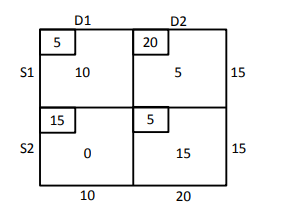
\includegraphics[width=0.75\columnwidth]{chapters/10/7/2/4/figs/fig.png}
 \end{center}
\caption{}
\label{fig:10/7/2/4Fig1}
\end{figure}
\fi

\item Find the position vector of the mid point of the vector joining the points $\vec{P}$(2, 3, 4)
and $\vec{Q}$(4, 1, –2).
\\
\solution
		\begin{enumerate}[label=\thesubsection.\arabic*,ref=\thesubsection.\theenumi]
\item Find the coordinates of the point which divides the join of $(-1,7) $ and $ (4,-3)$ in the ratio 2:3.
	\\
		\solution
	\begin{enumerate}[label=\thesubsection.\arabic*,ref=\thesubsection.\theenumi]
\item Find the coordinates of the point which divides the join of $(-1,7) $ and $ (4,-3)$ in the ratio 2:3.
	\\
		\solution
	\input{chapters/10/7/2/1/section.tex}
\item Find the coordinates of the point $\vec{R}$ on the line segment joining the points $\vec{P}(-1,3)$ and $\vec{Q}(2,5)$ such that $PR=\frac{3}{5}PQ$.
\item Find the ratio in which the point $\vec{P}\brak{\frac{3}{4},\frac{5}{12}}$ divides the line segment joining the points $\vec{A}\brak{\frac{1}{2},\frac{3}{2}}$ and $ \vec{B}(2,-5)$.
\item Find the coordinates of the point which divides the line segment joining the points $(4,-3)$ and $(8,5)$ in the ratio $3:1$ internally.
\item Find the coordinates of the point $\vec{P}$ on $AD$ such that $AP : PD = 2 : 1$.
\item If the point $\vec{P} (2, 1)$ lies on the line segment joining points $\vec{A} (4, 2)$  and $ \vec{B} (8, 4)$,
then
\begin{enumerate}
	\item $AP =\frac{1}{3}{AB}$ 
\item ${AP}={PE}$
\item ${PB}=\frac{1}{3}{AB}$
\item${AP}=\frac{1}{2}{AB}$
 \end{enumerate}
\item Find the ratio in which the line segment joining the points $(-3,10)$  and  $(6,-8)$  is divided by $ (-1,6)$.
	\\
		\solution
	\input{chapters/10/7/2/4/section.tex}
\item Find the position vector of the mid point of the vector joining the points $\vec{P}$(2, 3, 4)
and $\vec{Q}$(4, 1, –2).
\\
\solution
		\input{chapters/12/10/2/16/section.tex}
\item Let $\vec{A}(4, 2), \vec{B}(6, 5)$  and $ \vec{C}(1, 4)$ be the vertices of $\triangle ABC$.
\begin{enumerate}
\item If $\vec{A}$ and  $\vec{B}$ are $(-2,-2)$ and  $(2,-4)$, respectively, find the coordinates of $\vec{P}$ such that $AP= \frac {3}{7}AB$  and $ \vec{P}$ lies on the line segment $AB$.
	\\
		\solution
	\input{chapters/10/7/2/8/section.tex}
\item Find the coordinates of the points which divide the line segment joining $A(-2,2)$  and  $\vec{B}(2,8)$ into four equal parts.
	\\
		\solution
	\input{chapters/10/7/2/9/section.tex}
\item In what ratio does the point $(-4,6)$ divide the line segment joining the points $\vec{A}(-6,0)$ and $\vec{B}(3,-8)$?
\item Given that $\vec{P}(3,2,-4), \vec{Q}(5,4,-6)$ and $\vec{R}(9,8,-10)$ are collinear. Find the ratio in which $\vec{Q}$ divides $PR$.
\item Points $\vec{A}(-6,10),\vec{B}(-4,6)$  and  $\vec{C}(3,-8)$ are collinear such that $AB=  \frac{2}{9}AC$.
\item The point which divides the line segment joining the points $\vec{P} (7, –6) $  and  $\vec{Q}(3, 4)$ in the 
ratio 1 : 2 internally lies in  which quadrant?
\item Find the coordinates of the points of trisection of the line segment joining $(4,-1)$  and  $(-2,3)$.
	\\
		\solution
	\input{chapters/10/7/2/2/section.tex}
\item Find the coordinates of the points which trisect the line segment joining the points $\vec{P}(4,2,-6)$ and $\vec{Q}(10,-16,6)$.
\item Find the coordinates of the points of trisection (i.e. points dividing to three equal parts) of the line segment joining the points $\vec{A}(2,-2)$ and $\vec{B}(-7,4)$.
\item Point $\vec{P}(5,-3)$ is one of the two points of trisection of line segment joining the points $\vec{A}(7,-2)$ and $\vec{B}(1,-5)$
\item Find the position vector of a point $\vec{R}$ which divides the line joining two points $\vec{P}$
and $\vec{Q}$ whose position vectors are $\hat{i}+2\hat{j}-\hat{k}$ and $-\hat{i}+\hat{j}+\hat{k}$ respectively, in the
ratio 2 : 1
\begin{enumerate}
    \item  internally
    \item  externally
\end{enumerate}
%\solution
%		\input{chapters/12/10/2/15/section.tex}
\item Find the coordinates of the point which divides the line segment joining the points which divides the line segment joining  the points $(-2,3,5)$ and $(1,-4,6)$ in the ratio 
\begin{enumerate}
\item $2:3$ internally,
\item $2:3$ externally
\end{enumerate}
\item Find the coordinates of the point which divides the line segment joining the points $(1,-2,3)$ and $(3,4,-5)$ in the ratio $2:3$
\begin{enumerate}
\item internally, and
\item externally
\end{enumerate}
\item Consider two points $\vec{P}$ and $\vec{Q}$ with position vectors $\overrightarrow{OP} = 3\overrightarrow{a}-2\overrightarrow{b}$ and $\overrightarrow{OQ}=\overrightarrow{a}+\overrightarrow{b}$. Find the position vector of a point $\vec{R}$ which divides the line joining $\vec{P}$ and $\vec{Q}$ in the ratio $2:1$, 
\begin{enumerate}
\item internally, and 
\item externally.
\end{enumerate}
\item The median from $\vec{A}$ meets $BC$ at $\vec{D}$. Find the coordinates of the point $\vec{D}$.
\item Find the coordinates of points $\vec{Q}$ and $\vec{R}$ on medians $BE$ and $CF$ respectively such that $BQ : QE = 2 : 1$  and  $CR : RF = 2 : 1$.
\item What do you observe?
\item If $\vec{A}, \vec{B}$ and $\vec{C}$  are the vertices of $\triangle ABC$, find the coordinates of the centroid of the triangle.
\end{enumerate}
\solution
	\input{chapters/10/7/4/7/section.tex}
\item If $\vec{P}(9a-2,-b)$ divides line segment joining $\vec{A}(3a+1,-3)$ and $\vec{B}(8a,5)$ in the ratio 3:1, find the values of $a$ and $b$.
\item Find the position vector of a point $\vec{R}$ which divides the line joining two points $\vec{P}$ and $\vec{Q}$ whose position vectors are $2\vec{a}+\vec{b}$ and $\vec{a}-3\vec{b}$ externally in the ratio $1:2$.
\item The position vector of the point which divides the join of points 2$\vec{a}$-3$\vec{b}$ $\text{and}$ $\vec{a}+\vec{b}$ in the ratio 3:1 is \rule{1cm}{0.1pt}.
\item If $\vec{a}$ and $\vec{b}$ are the postion vectors of $\vec{A}$ and $\vec{B}$, respectively, find the position vector of a point $\vec{C}$ in $BA$ produced such that $BC=1.5BA$.
\item Find the position vector of a point $\vec{R}$ which divides the line joining two points $\vec{P}$ and $\vec{Q}$ whose position vectors are $(2\vec{a}+\vec{b})$ and $(\vec{a}-3\vec{b})$
externally in the ratio 1 : 2. Also, show that $\vec{P}$ is the mid point of the line segment $RQ$.
\end{enumerate}

\item Find the coordinates of the point $\vec{R}$ on the line segment joining the points $\vec{P}(-1,3)$ and $\vec{Q}(2,5)$ such that $PR=\frac{3}{5}PQ$.
\item Find the ratio in which the point $\vec{P}\brak{\frac{3}{4},\frac{5}{12}}$ divides the line segment joining the points $\vec{A}\brak{\frac{1}{2},\frac{3}{2}}$ and $ \vec{B}(2,-5)$.
\item Find the coordinates of the point which divides the line segment joining the points $(4,-3)$ and $(8,5)$ in the ratio $3:1$ internally.
\item Find the coordinates of the point $\vec{P}$ on $AD$ such that $AP : PD = 2 : 1$.
\item If the point $\vec{P} (2, 1)$ lies on the line segment joining points $\vec{A} (4, 2)$  and $ \vec{B} (8, 4)$,
then
\begin{enumerate}
	\item $AP =\frac{1}{3}{AB}$ 
\item ${AP}={PE}$
\item ${PB}=\frac{1}{3}{AB}$
\item${AP}=\frac{1}{2}{AB}$
 \end{enumerate}
\item Find the ratio in which the line segment joining the points $(-3,10)$  and  $(6,-8)$  is divided by $ (-1,6)$.
	\\
		\solution
	\iffalse
Using section formula,
\begin{align}
         \myvec{-1\\6} &=\frac{{\myvec{-3\\10}+k\myvec{6\\-8}}}{1+k}\\
	 \implies 7k\myvec{1 \\ -2} &= 2\myvec{1 \\ -2}
	 \\
	 \text{or, } k &= \frac{2}{7}.
\end{align}
\fi
In 
			\eqref{eq:section_formula-k}, substituting
			\begin{align}
				\vec{B} &= \myvec{-3\\10}, \vec{C} = \myvec{6\\-8}, \vec{D} = \myvec{-1\\6},
				\\
				k &= \frac{\myvec{-2 & 4}\myvec{-7 \\ 14}}{\norm{\myvec{-7 \\ 14}}^2} = \frac{2}{7}
			\end{align}
\iffalse
See \figref{fig:10/7/2/4Fig1}.
\begin{figure}[H]
 \begin{center}
  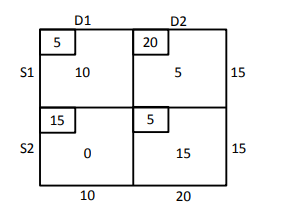
\includegraphics[width=0.75\columnwidth]{chapters/10/7/2/4/figs/fig.png}
 \end{center}
\caption{}
\label{fig:10/7/2/4Fig1}
\end{figure}
\fi

\item Find the position vector of the mid point of the vector joining the points $\vec{P}$(2, 3, 4)
and $\vec{Q}$(4, 1, –2).
\\
\solution
		\begin{enumerate}[label=\thesubsection.\arabic*,ref=\thesubsection.\theenumi]
\item Find the coordinates of the point which divides the join of $(-1,7) $ and $ (4,-3)$ in the ratio 2:3.
	\\
		\solution
	\input{chapters/10/7/2/1/section.tex}
\item Find the coordinates of the point $\vec{R}$ on the line segment joining the points $\vec{P}(-1,3)$ and $\vec{Q}(2,5)$ such that $PR=\frac{3}{5}PQ$.
\item Find the ratio in which the point $\vec{P}\brak{\frac{3}{4},\frac{5}{12}}$ divides the line segment joining the points $\vec{A}\brak{\frac{1}{2},\frac{3}{2}}$ and $ \vec{B}(2,-5)$.
\item Find the coordinates of the point which divides the line segment joining the points $(4,-3)$ and $(8,5)$ in the ratio $3:1$ internally.
\item Find the coordinates of the point $\vec{P}$ on $AD$ such that $AP : PD = 2 : 1$.
\item If the point $\vec{P} (2, 1)$ lies on the line segment joining points $\vec{A} (4, 2)$  and $ \vec{B} (8, 4)$,
then
\begin{enumerate}
	\item $AP =\frac{1}{3}{AB}$ 
\item ${AP}={PE}$
\item ${PB}=\frac{1}{3}{AB}$
\item${AP}=\frac{1}{2}{AB}$
 \end{enumerate}
\item Find the ratio in which the line segment joining the points $(-3,10)$  and  $(6,-8)$  is divided by $ (-1,6)$.
	\\
		\solution
	\input{chapters/10/7/2/4/section.tex}
\item Find the position vector of the mid point of the vector joining the points $\vec{P}$(2, 3, 4)
and $\vec{Q}$(4, 1, –2).
\\
\solution
		\input{chapters/12/10/2/16/section.tex}
\item Let $\vec{A}(4, 2), \vec{B}(6, 5)$  and $ \vec{C}(1, 4)$ be the vertices of $\triangle ABC$.
\begin{enumerate}
\item If $\vec{A}$ and  $\vec{B}$ are $(-2,-2)$ and  $(2,-4)$, respectively, find the coordinates of $\vec{P}$ such that $AP= \frac {3}{7}AB$  and $ \vec{P}$ lies on the line segment $AB$.
	\\
		\solution
	\input{chapters/10/7/2/8/section.tex}
\item Find the coordinates of the points which divide the line segment joining $A(-2,2)$  and  $\vec{B}(2,8)$ into four equal parts.
	\\
		\solution
	\input{chapters/10/7/2/9/section.tex}
\item In what ratio does the point $(-4,6)$ divide the line segment joining the points $\vec{A}(-6,0)$ and $\vec{B}(3,-8)$?
\item Given that $\vec{P}(3,2,-4), \vec{Q}(5,4,-6)$ and $\vec{R}(9,8,-10)$ are collinear. Find the ratio in which $\vec{Q}$ divides $PR$.
\item Points $\vec{A}(-6,10),\vec{B}(-4,6)$  and  $\vec{C}(3,-8)$ are collinear such that $AB=  \frac{2}{9}AC$.
\item The point which divides the line segment joining the points $\vec{P} (7, –6) $  and  $\vec{Q}(3, 4)$ in the 
ratio 1 : 2 internally lies in  which quadrant?
\item Find the coordinates of the points of trisection of the line segment joining $(4,-1)$  and  $(-2,3)$.
	\\
		\solution
	\input{chapters/10/7/2/2/section.tex}
\item Find the coordinates of the points which trisect the line segment joining the points $\vec{P}(4,2,-6)$ and $\vec{Q}(10,-16,6)$.
\item Find the coordinates of the points of trisection (i.e. points dividing to three equal parts) of the line segment joining the points $\vec{A}(2,-2)$ and $\vec{B}(-7,4)$.
\item Point $\vec{P}(5,-3)$ is one of the two points of trisection of line segment joining the points $\vec{A}(7,-2)$ and $\vec{B}(1,-5)$
\item Find the position vector of a point $\vec{R}$ which divides the line joining two points $\vec{P}$
and $\vec{Q}$ whose position vectors are $\hat{i}+2\hat{j}-\hat{k}$ and $-\hat{i}+\hat{j}+\hat{k}$ respectively, in the
ratio 2 : 1
\begin{enumerate}
    \item  internally
    \item  externally
\end{enumerate}
%\solution
%		\input{chapters/12/10/2/15/section.tex}
\item Find the coordinates of the point which divides the line segment joining the points which divides the line segment joining  the points $(-2,3,5)$ and $(1,-4,6)$ in the ratio 
\begin{enumerate}
\item $2:3$ internally,
\item $2:3$ externally
\end{enumerate}
\item Find the coordinates of the point which divides the line segment joining the points $(1,-2,3)$ and $(3,4,-5)$ in the ratio $2:3$
\begin{enumerate}
\item internally, and
\item externally
\end{enumerate}
\item Consider two points $\vec{P}$ and $\vec{Q}$ with position vectors $\overrightarrow{OP} = 3\overrightarrow{a}-2\overrightarrow{b}$ and $\overrightarrow{OQ}=\overrightarrow{a}+\overrightarrow{b}$. Find the position vector of a point $\vec{R}$ which divides the line joining $\vec{P}$ and $\vec{Q}$ in the ratio $2:1$, 
\begin{enumerate}
\item internally, and 
\item externally.
\end{enumerate}
\item The median from $\vec{A}$ meets $BC$ at $\vec{D}$. Find the coordinates of the point $\vec{D}$.
\item Find the coordinates of points $\vec{Q}$ and $\vec{R}$ on medians $BE$ and $CF$ respectively such that $BQ : QE = 2 : 1$  and  $CR : RF = 2 : 1$.
\item What do you observe?
\item If $\vec{A}, \vec{B}$ and $\vec{C}$  are the vertices of $\triangle ABC$, find the coordinates of the centroid of the triangle.
\end{enumerate}
\solution
	\input{chapters/10/7/4/7/section.tex}
\item If $\vec{P}(9a-2,-b)$ divides line segment joining $\vec{A}(3a+1,-3)$ and $\vec{B}(8a,5)$ in the ratio 3:1, find the values of $a$ and $b$.
\item Find the position vector of a point $\vec{R}$ which divides the line joining two points $\vec{P}$ and $\vec{Q}$ whose position vectors are $2\vec{a}+\vec{b}$ and $\vec{a}-3\vec{b}$ externally in the ratio $1:2$.
\item The position vector of the point which divides the join of points 2$\vec{a}$-3$\vec{b}$ $\text{and}$ $\vec{a}+\vec{b}$ in the ratio 3:1 is \rule{1cm}{0.1pt}.
\item If $\vec{a}$ and $\vec{b}$ are the postion vectors of $\vec{A}$ and $\vec{B}$, respectively, find the position vector of a point $\vec{C}$ in $BA$ produced such that $BC=1.5BA$.
\item Find the position vector of a point $\vec{R}$ which divides the line joining two points $\vec{P}$ and $\vec{Q}$ whose position vectors are $(2\vec{a}+\vec{b})$ and $(\vec{a}-3\vec{b})$
externally in the ratio 1 : 2. Also, show that $\vec{P}$ is the mid point of the line segment $RQ$.
\end{enumerate}

\item Let $\vec{A}(4, 2), \vec{B}(6, 5)$  and $ \vec{C}(1, 4)$ be the vertices of $\triangle ABC$.
\begin{enumerate}
\item If $\vec{A}$ and  $\vec{B}$ are $(-2,-2)$ and  $(2,-4)$, respectively, find the coordinates of $\vec{P}$ such that $AP= \frac {3}{7}AB$  and $ \vec{P}$ lies on the line segment $AB$.
	\\
		\solution
	\begin{enumerate}[label=\thesubsection.\arabic*,ref=\thesubsection.\theenumi]
\item Find the coordinates of the point which divides the join of $(-1,7) $ and $ (4,-3)$ in the ratio 2:3.
	\\
		\solution
	\input{chapters/10/7/2/1/section.tex}
\item Find the coordinates of the point $\vec{R}$ on the line segment joining the points $\vec{P}(-1,3)$ and $\vec{Q}(2,5)$ such that $PR=\frac{3}{5}PQ$.
\item Find the ratio in which the point $\vec{P}\brak{\frac{3}{4},\frac{5}{12}}$ divides the line segment joining the points $\vec{A}\brak{\frac{1}{2},\frac{3}{2}}$ and $ \vec{B}(2,-5)$.
\item Find the coordinates of the point which divides the line segment joining the points $(4,-3)$ and $(8,5)$ in the ratio $3:1$ internally.
\item Find the coordinates of the point $\vec{P}$ on $AD$ such that $AP : PD = 2 : 1$.
\item If the point $\vec{P} (2, 1)$ lies on the line segment joining points $\vec{A} (4, 2)$  and $ \vec{B} (8, 4)$,
then
\begin{enumerate}
	\item $AP =\frac{1}{3}{AB}$ 
\item ${AP}={PE}$
\item ${PB}=\frac{1}{3}{AB}$
\item${AP}=\frac{1}{2}{AB}$
 \end{enumerate}
\item Find the ratio in which the line segment joining the points $(-3,10)$  and  $(6,-8)$  is divided by $ (-1,6)$.
	\\
		\solution
	\input{chapters/10/7/2/4/section.tex}
\item Find the position vector of the mid point of the vector joining the points $\vec{P}$(2, 3, 4)
and $\vec{Q}$(4, 1, –2).
\\
\solution
		\input{chapters/12/10/2/16/section.tex}
\item Let $\vec{A}(4, 2), \vec{B}(6, 5)$  and $ \vec{C}(1, 4)$ be the vertices of $\triangle ABC$.
\begin{enumerate}
\item If $\vec{A}$ and  $\vec{B}$ are $(-2,-2)$ and  $(2,-4)$, respectively, find the coordinates of $\vec{P}$ such that $AP= \frac {3}{7}AB$  and $ \vec{P}$ lies on the line segment $AB$.
	\\
		\solution
	\input{chapters/10/7/2/8/section.tex}
\item Find the coordinates of the points which divide the line segment joining $A(-2,2)$  and  $\vec{B}(2,8)$ into four equal parts.
	\\
		\solution
	\input{chapters/10/7/2/9/section.tex}
\item In what ratio does the point $(-4,6)$ divide the line segment joining the points $\vec{A}(-6,0)$ and $\vec{B}(3,-8)$?
\item Given that $\vec{P}(3,2,-4), \vec{Q}(5,4,-6)$ and $\vec{R}(9,8,-10)$ are collinear. Find the ratio in which $\vec{Q}$ divides $PR$.
\item Points $\vec{A}(-6,10),\vec{B}(-4,6)$  and  $\vec{C}(3,-8)$ are collinear such that $AB=  \frac{2}{9}AC$.
\item The point which divides the line segment joining the points $\vec{P} (7, –6) $  and  $\vec{Q}(3, 4)$ in the 
ratio 1 : 2 internally lies in  which quadrant?
\item Find the coordinates of the points of trisection of the line segment joining $(4,-1)$  and  $(-2,3)$.
	\\
		\solution
	\input{chapters/10/7/2/2/section.tex}
\item Find the coordinates of the points which trisect the line segment joining the points $\vec{P}(4,2,-6)$ and $\vec{Q}(10,-16,6)$.
\item Find the coordinates of the points of trisection (i.e. points dividing to three equal parts) of the line segment joining the points $\vec{A}(2,-2)$ and $\vec{B}(-7,4)$.
\item Point $\vec{P}(5,-3)$ is one of the two points of trisection of line segment joining the points $\vec{A}(7,-2)$ and $\vec{B}(1,-5)$
\item Find the position vector of a point $\vec{R}$ which divides the line joining two points $\vec{P}$
and $\vec{Q}$ whose position vectors are $\hat{i}+2\hat{j}-\hat{k}$ and $-\hat{i}+\hat{j}+\hat{k}$ respectively, in the
ratio 2 : 1
\begin{enumerate}
    \item  internally
    \item  externally
\end{enumerate}
%\solution
%		\input{chapters/12/10/2/15/section.tex}
\item Find the coordinates of the point which divides the line segment joining the points which divides the line segment joining  the points $(-2,3,5)$ and $(1,-4,6)$ in the ratio 
\begin{enumerate}
\item $2:3$ internally,
\item $2:3$ externally
\end{enumerate}
\item Find the coordinates of the point which divides the line segment joining the points $(1,-2,3)$ and $(3,4,-5)$ in the ratio $2:3$
\begin{enumerate}
\item internally, and
\item externally
\end{enumerate}
\item Consider two points $\vec{P}$ and $\vec{Q}$ with position vectors $\overrightarrow{OP} = 3\overrightarrow{a}-2\overrightarrow{b}$ and $\overrightarrow{OQ}=\overrightarrow{a}+\overrightarrow{b}$. Find the position vector of a point $\vec{R}$ which divides the line joining $\vec{P}$ and $\vec{Q}$ in the ratio $2:1$, 
\begin{enumerate}
\item internally, and 
\item externally.
\end{enumerate}
\item The median from $\vec{A}$ meets $BC$ at $\vec{D}$. Find the coordinates of the point $\vec{D}$.
\item Find the coordinates of points $\vec{Q}$ and $\vec{R}$ on medians $BE$ and $CF$ respectively such that $BQ : QE = 2 : 1$  and  $CR : RF = 2 : 1$.
\item What do you observe?
\item If $\vec{A}, \vec{B}$ and $\vec{C}$  are the vertices of $\triangle ABC$, find the coordinates of the centroid of the triangle.
\end{enumerate}
\solution
	\input{chapters/10/7/4/7/section.tex}
\item If $\vec{P}(9a-2,-b)$ divides line segment joining $\vec{A}(3a+1,-3)$ and $\vec{B}(8a,5)$ in the ratio 3:1, find the values of $a$ and $b$.
\item Find the position vector of a point $\vec{R}$ which divides the line joining two points $\vec{P}$ and $\vec{Q}$ whose position vectors are $2\vec{a}+\vec{b}$ and $\vec{a}-3\vec{b}$ externally in the ratio $1:2$.
\item The position vector of the point which divides the join of points 2$\vec{a}$-3$\vec{b}$ $\text{and}$ $\vec{a}+\vec{b}$ in the ratio 3:1 is \rule{1cm}{0.1pt}.
\item If $\vec{a}$ and $\vec{b}$ are the postion vectors of $\vec{A}$ and $\vec{B}$, respectively, find the position vector of a point $\vec{C}$ in $BA$ produced such that $BC=1.5BA$.
\item Find the position vector of a point $\vec{R}$ which divides the line joining two points $\vec{P}$ and $\vec{Q}$ whose position vectors are $(2\vec{a}+\vec{b})$ and $(\vec{a}-3\vec{b})$
externally in the ratio 1 : 2. Also, show that $\vec{P}$ is the mid point of the line segment $RQ$.
\end{enumerate}

\item Find the coordinates of the points which divide the line segment joining $A(-2,2)$  and  $\vec{B}(2,8)$ into four equal parts.
	\\
		\solution
	\begin{enumerate}[label=\thesubsection.\arabic*,ref=\thesubsection.\theenumi]
\item Find the coordinates of the point which divides the join of $(-1,7) $ and $ (4,-3)$ in the ratio 2:3.
	\\
		\solution
	\input{chapters/10/7/2/1/section.tex}
\item Find the coordinates of the point $\vec{R}$ on the line segment joining the points $\vec{P}(-1,3)$ and $\vec{Q}(2,5)$ such that $PR=\frac{3}{5}PQ$.
\item Find the ratio in which the point $\vec{P}\brak{\frac{3}{4},\frac{5}{12}}$ divides the line segment joining the points $\vec{A}\brak{\frac{1}{2},\frac{3}{2}}$ and $ \vec{B}(2,-5)$.
\item Find the coordinates of the point which divides the line segment joining the points $(4,-3)$ and $(8,5)$ in the ratio $3:1$ internally.
\item Find the coordinates of the point $\vec{P}$ on $AD$ such that $AP : PD = 2 : 1$.
\item If the point $\vec{P} (2, 1)$ lies on the line segment joining points $\vec{A} (4, 2)$  and $ \vec{B} (8, 4)$,
then
\begin{enumerate}
	\item $AP =\frac{1}{3}{AB}$ 
\item ${AP}={PE}$
\item ${PB}=\frac{1}{3}{AB}$
\item${AP}=\frac{1}{2}{AB}$
 \end{enumerate}
\item Find the ratio in which the line segment joining the points $(-3,10)$  and  $(6,-8)$  is divided by $ (-1,6)$.
	\\
		\solution
	\input{chapters/10/7/2/4/section.tex}
\item Find the position vector of the mid point of the vector joining the points $\vec{P}$(2, 3, 4)
and $\vec{Q}$(4, 1, –2).
\\
\solution
		\input{chapters/12/10/2/16/section.tex}
\item Let $\vec{A}(4, 2), \vec{B}(6, 5)$  and $ \vec{C}(1, 4)$ be the vertices of $\triangle ABC$.
\begin{enumerate}
\item If $\vec{A}$ and  $\vec{B}$ are $(-2,-2)$ and  $(2,-4)$, respectively, find the coordinates of $\vec{P}$ such that $AP= \frac {3}{7}AB$  and $ \vec{P}$ lies on the line segment $AB$.
	\\
		\solution
	\input{chapters/10/7/2/8/section.tex}
\item Find the coordinates of the points which divide the line segment joining $A(-2,2)$  and  $\vec{B}(2,8)$ into four equal parts.
	\\
		\solution
	\input{chapters/10/7/2/9/section.tex}
\item In what ratio does the point $(-4,6)$ divide the line segment joining the points $\vec{A}(-6,0)$ and $\vec{B}(3,-8)$?
\item Given that $\vec{P}(3,2,-4), \vec{Q}(5,4,-6)$ and $\vec{R}(9,8,-10)$ are collinear. Find the ratio in which $\vec{Q}$ divides $PR$.
\item Points $\vec{A}(-6,10),\vec{B}(-4,6)$  and  $\vec{C}(3,-8)$ are collinear such that $AB=  \frac{2}{9}AC$.
\item The point which divides the line segment joining the points $\vec{P} (7, –6) $  and  $\vec{Q}(3, 4)$ in the 
ratio 1 : 2 internally lies in  which quadrant?
\item Find the coordinates of the points of trisection of the line segment joining $(4,-1)$  and  $(-2,3)$.
	\\
		\solution
	\input{chapters/10/7/2/2/section.tex}
\item Find the coordinates of the points which trisect the line segment joining the points $\vec{P}(4,2,-6)$ and $\vec{Q}(10,-16,6)$.
\item Find the coordinates of the points of trisection (i.e. points dividing to three equal parts) of the line segment joining the points $\vec{A}(2,-2)$ and $\vec{B}(-7,4)$.
\item Point $\vec{P}(5,-3)$ is one of the two points of trisection of line segment joining the points $\vec{A}(7,-2)$ and $\vec{B}(1,-5)$
\item Find the position vector of a point $\vec{R}$ which divides the line joining two points $\vec{P}$
and $\vec{Q}$ whose position vectors are $\hat{i}+2\hat{j}-\hat{k}$ and $-\hat{i}+\hat{j}+\hat{k}$ respectively, in the
ratio 2 : 1
\begin{enumerate}
    \item  internally
    \item  externally
\end{enumerate}
%\solution
%		\input{chapters/12/10/2/15/section.tex}
\item Find the coordinates of the point which divides the line segment joining the points which divides the line segment joining  the points $(-2,3,5)$ and $(1,-4,6)$ in the ratio 
\begin{enumerate}
\item $2:3$ internally,
\item $2:3$ externally
\end{enumerate}
\item Find the coordinates of the point which divides the line segment joining the points $(1,-2,3)$ and $(3,4,-5)$ in the ratio $2:3$
\begin{enumerate}
\item internally, and
\item externally
\end{enumerate}
\item Consider two points $\vec{P}$ and $\vec{Q}$ with position vectors $\overrightarrow{OP} = 3\overrightarrow{a}-2\overrightarrow{b}$ and $\overrightarrow{OQ}=\overrightarrow{a}+\overrightarrow{b}$. Find the position vector of a point $\vec{R}$ which divides the line joining $\vec{P}$ and $\vec{Q}$ in the ratio $2:1$, 
\begin{enumerate}
\item internally, and 
\item externally.
\end{enumerate}
\item The median from $\vec{A}$ meets $BC$ at $\vec{D}$. Find the coordinates of the point $\vec{D}$.
\item Find the coordinates of points $\vec{Q}$ and $\vec{R}$ on medians $BE$ and $CF$ respectively such that $BQ : QE = 2 : 1$  and  $CR : RF = 2 : 1$.
\item What do you observe?
\item If $\vec{A}, \vec{B}$ and $\vec{C}$  are the vertices of $\triangle ABC$, find the coordinates of the centroid of the triangle.
\end{enumerate}
\solution
	\input{chapters/10/7/4/7/section.tex}
\item If $\vec{P}(9a-2,-b)$ divides line segment joining $\vec{A}(3a+1,-3)$ and $\vec{B}(8a,5)$ in the ratio 3:1, find the values of $a$ and $b$.
\item Find the position vector of a point $\vec{R}$ which divides the line joining two points $\vec{P}$ and $\vec{Q}$ whose position vectors are $2\vec{a}+\vec{b}$ and $\vec{a}-3\vec{b}$ externally in the ratio $1:2$.
\item The position vector of the point which divides the join of points 2$\vec{a}$-3$\vec{b}$ $\text{and}$ $\vec{a}+\vec{b}$ in the ratio 3:1 is \rule{1cm}{0.1pt}.
\item If $\vec{a}$ and $\vec{b}$ are the postion vectors of $\vec{A}$ and $\vec{B}$, respectively, find the position vector of a point $\vec{C}$ in $BA$ produced such that $BC=1.5BA$.
\item Find the position vector of a point $\vec{R}$ which divides the line joining two points $\vec{P}$ and $\vec{Q}$ whose position vectors are $(2\vec{a}+\vec{b})$ and $(\vec{a}-3\vec{b})$
externally in the ratio 1 : 2. Also, show that $\vec{P}$ is the mid point of the line segment $RQ$.
\end{enumerate}

\item In what ratio does the point $(-4,6)$ divide the line segment joining the points $\vec{A}(-6,0)$ and $\vec{B}(3,-8)$?
\item Given that $\vec{P}(3,2,-4), \vec{Q}(5,4,-6)$ and $\vec{R}(9,8,-10)$ are collinear. Find the ratio in which $\vec{Q}$ divides $PR$.
\item Points $\vec{A}(-6,10),\vec{B}(-4,6)$  and  $\vec{C}(3,-8)$ are collinear such that $AB=  \frac{2}{9}AC$.
\item The point which divides the line segment joining the points $\vec{P} (7, –6) $  and  $\vec{Q}(3, 4)$ in the 
ratio 1 : 2 internally lies in  which quadrant?
\item Find the coordinates of the points of trisection of the line segment joining $(4,-1)$  and  $(-2,3)$.
	\\
		\solution
	Using section formula,
\begin{align}
\vec{R}=\frac{1}{1+\frac{1}{2}}\brak{\myvec{4\\-1}+\frac{1}{2}\myvec{-2\\3}}
=\myvec{2\\ \frac{1}{3}}\\
\vec{S}=\frac{1}{1+\frac{2}{1}}\brak{\myvec{4\\-1}+\frac{2}{1}\myvec{-2\\3}}
=\myvec{0\\ \frac{5}{3}}
\end{align}
which are the desired points of trisection.
\iffalse
See
		\figref{fig:chapters/10/7/2/2/Figure}
\begin{figure}[H]
\centering
\includegraphics[width=0.75\columnwidth]{chapters/10/7/2/2/figs/dj.pdf}
\caption{}
		\label{fig:chapters/10/7/2/2/Figure}
\end{figure}
\fi

\item Find the coordinates of the points which trisect the line segment joining the points $\vec{P}(4,2,-6)$ and $\vec{Q}(10,-16,6)$.
\item Find the coordinates of the points of trisection (i.e. points dividing to three equal parts) of the line segment joining the points $\vec{A}(2,-2)$ and $\vec{B}(-7,4)$.
\item Point $\vec{P}(5,-3)$ is one of the two points of trisection of line segment joining the points $\vec{A}(7,-2)$ and $\vec{B}(1,-5)$
\item Find the position vector of a point $\vec{R}$ which divides the line joining two points $\vec{P}$
and $\vec{Q}$ whose position vectors are $\hat{i}+2\hat{j}-\hat{k}$ and $-\hat{i}+\hat{j}+\hat{k}$ respectively, in the
ratio 2 : 1
\begin{enumerate}
    \item  internally
    \item  externally
\end{enumerate}
%\solution
%		\begin{enumerate}[label=\thesubsection.\arabic*,ref=\thesubsection.\theenumi]
\item Find the coordinates of the point which divides the join of $(-1,7) $ and $ (4,-3)$ in the ratio 2:3.
	\\
		\solution
	\input{chapters/10/7/2/1/section.tex}
\item Find the coordinates of the point $\vec{R}$ on the line segment joining the points $\vec{P}(-1,3)$ and $\vec{Q}(2,5)$ such that $PR=\frac{3}{5}PQ$.
\item Find the ratio in which the point $\vec{P}\brak{\frac{3}{4},\frac{5}{12}}$ divides the line segment joining the points $\vec{A}\brak{\frac{1}{2},\frac{3}{2}}$ and $ \vec{B}(2,-5)$.
\item Find the coordinates of the point which divides the line segment joining the points $(4,-3)$ and $(8,5)$ in the ratio $3:1$ internally.
\item Find the coordinates of the point $\vec{P}$ on $AD$ such that $AP : PD = 2 : 1$.
\item If the point $\vec{P} (2, 1)$ lies on the line segment joining points $\vec{A} (4, 2)$  and $ \vec{B} (8, 4)$,
then
\begin{enumerate}
	\item $AP =\frac{1}{3}{AB}$ 
\item ${AP}={PE}$
\item ${PB}=\frac{1}{3}{AB}$
\item${AP}=\frac{1}{2}{AB}$
 \end{enumerate}
\item Find the ratio in which the line segment joining the points $(-3,10)$  and  $(6,-8)$  is divided by $ (-1,6)$.
	\\
		\solution
	\input{chapters/10/7/2/4/section.tex}
\item Find the position vector of the mid point of the vector joining the points $\vec{P}$(2, 3, 4)
and $\vec{Q}$(4, 1, –2).
\\
\solution
		\input{chapters/12/10/2/16/section.tex}
\item Let $\vec{A}(4, 2), \vec{B}(6, 5)$  and $ \vec{C}(1, 4)$ be the vertices of $\triangle ABC$.
\begin{enumerate}
\item If $\vec{A}$ and  $\vec{B}$ are $(-2,-2)$ and  $(2,-4)$, respectively, find the coordinates of $\vec{P}$ such that $AP= \frac {3}{7}AB$  and $ \vec{P}$ lies on the line segment $AB$.
	\\
		\solution
	\input{chapters/10/7/2/8/section.tex}
\item Find the coordinates of the points which divide the line segment joining $A(-2,2)$  and  $\vec{B}(2,8)$ into four equal parts.
	\\
		\solution
	\input{chapters/10/7/2/9/section.tex}
\item In what ratio does the point $(-4,6)$ divide the line segment joining the points $\vec{A}(-6,0)$ and $\vec{B}(3,-8)$?
\item Given that $\vec{P}(3,2,-4), \vec{Q}(5,4,-6)$ and $\vec{R}(9,8,-10)$ are collinear. Find the ratio in which $\vec{Q}$ divides $PR$.
\item Points $\vec{A}(-6,10),\vec{B}(-4,6)$  and  $\vec{C}(3,-8)$ are collinear such that $AB=  \frac{2}{9}AC$.
\item The point which divides the line segment joining the points $\vec{P} (7, –6) $  and  $\vec{Q}(3, 4)$ in the 
ratio 1 : 2 internally lies in  which quadrant?
\item Find the coordinates of the points of trisection of the line segment joining $(4,-1)$  and  $(-2,3)$.
	\\
		\solution
	\input{chapters/10/7/2/2/section.tex}
\item Find the coordinates of the points which trisect the line segment joining the points $\vec{P}(4,2,-6)$ and $\vec{Q}(10,-16,6)$.
\item Find the coordinates of the points of trisection (i.e. points dividing to three equal parts) of the line segment joining the points $\vec{A}(2,-2)$ and $\vec{B}(-7,4)$.
\item Point $\vec{P}(5,-3)$ is one of the two points of trisection of line segment joining the points $\vec{A}(7,-2)$ and $\vec{B}(1,-5)$
\item Find the position vector of a point $\vec{R}$ which divides the line joining two points $\vec{P}$
and $\vec{Q}$ whose position vectors are $\hat{i}+2\hat{j}-\hat{k}$ and $-\hat{i}+\hat{j}+\hat{k}$ respectively, in the
ratio 2 : 1
\begin{enumerate}
    \item  internally
    \item  externally
\end{enumerate}
%\solution
%		\input{chapters/12/10/2/15/section.tex}
\item Find the coordinates of the point which divides the line segment joining the points which divides the line segment joining  the points $(-2,3,5)$ and $(1,-4,6)$ in the ratio 
\begin{enumerate}
\item $2:3$ internally,
\item $2:3$ externally
\end{enumerate}
\item Find the coordinates of the point which divides the line segment joining the points $(1,-2,3)$ and $(3,4,-5)$ in the ratio $2:3$
\begin{enumerate}
\item internally, and
\item externally
\end{enumerate}
\item Consider two points $\vec{P}$ and $\vec{Q}$ with position vectors $\overrightarrow{OP} = 3\overrightarrow{a}-2\overrightarrow{b}$ and $\overrightarrow{OQ}=\overrightarrow{a}+\overrightarrow{b}$. Find the position vector of a point $\vec{R}$ which divides the line joining $\vec{P}$ and $\vec{Q}$ in the ratio $2:1$, 
\begin{enumerate}
\item internally, and 
\item externally.
\end{enumerate}
\item The median from $\vec{A}$ meets $BC$ at $\vec{D}$. Find the coordinates of the point $\vec{D}$.
\item Find the coordinates of points $\vec{Q}$ and $\vec{R}$ on medians $BE$ and $CF$ respectively such that $BQ : QE = 2 : 1$  and  $CR : RF = 2 : 1$.
\item What do you observe?
\item If $\vec{A}, \vec{B}$ and $\vec{C}$  are the vertices of $\triangle ABC$, find the coordinates of the centroid of the triangle.
\end{enumerate}
\solution
	\input{chapters/10/7/4/7/section.tex}
\item If $\vec{P}(9a-2,-b)$ divides line segment joining $\vec{A}(3a+1,-3)$ and $\vec{B}(8a,5)$ in the ratio 3:1, find the values of $a$ and $b$.
\item Find the position vector of a point $\vec{R}$ which divides the line joining two points $\vec{P}$ and $\vec{Q}$ whose position vectors are $2\vec{a}+\vec{b}$ and $\vec{a}-3\vec{b}$ externally in the ratio $1:2$.
\item The position vector of the point which divides the join of points 2$\vec{a}$-3$\vec{b}$ $\text{and}$ $\vec{a}+\vec{b}$ in the ratio 3:1 is \rule{1cm}{0.1pt}.
\item If $\vec{a}$ and $\vec{b}$ are the postion vectors of $\vec{A}$ and $\vec{B}$, respectively, find the position vector of a point $\vec{C}$ in $BA$ produced such that $BC=1.5BA$.
\item Find the position vector of a point $\vec{R}$ which divides the line joining two points $\vec{P}$ and $\vec{Q}$ whose position vectors are $(2\vec{a}+\vec{b})$ and $(\vec{a}-3\vec{b})$
externally in the ratio 1 : 2. Also, show that $\vec{P}$ is the mid point of the line segment $RQ$.
\end{enumerate}

\item Find the coordinates of the point which divides the line segment joining the points which divides the line segment joining  the points $(-2,3,5)$ and $(1,-4,6)$ in the ratio 
\begin{enumerate}
\item $2:3$ internally,
\item $2:3$ externally
\end{enumerate}
\item Find the coordinates of the point which divides the line segment joining the points $(1,-2,3)$ and $(3,4,-5)$ in the ratio $2:3$
\begin{enumerate}
\item internally, and
\item externally
\end{enumerate}
\item Consider two points $\vec{P}$ and $\vec{Q}$ with position vectors $\overrightarrow{OP} = 3\overrightarrow{a}-2\overrightarrow{b}$ and $\overrightarrow{OQ}=\overrightarrow{a}+\overrightarrow{b}$. Find the position vector of a point $\vec{R}$ which divides the line joining $\vec{P}$ and $\vec{Q}$ in the ratio $2:1$, 
\begin{enumerate}
\item internally, and 
\item externally.
\end{enumerate}
\item The median from $\vec{A}$ meets $BC$ at $\vec{D}$. Find the coordinates of the point $\vec{D}$.
\item Find the coordinates of points $\vec{Q}$ and $\vec{R}$ on medians $BE$ and $CF$ respectively such that $BQ : QE = 2 : 1$  and  $CR : RF = 2 : 1$.
\item What do you observe?
\item If $\vec{A}, \vec{B}$ and $\vec{C}$  are the vertices of $\triangle ABC$, find the coordinates of the centroid of the triangle.
\end{enumerate}
\solution
	\begin{enumerate}[label=\thesubsection.\arabic*,ref=\thesubsection.\theenumi]
\item Find the coordinates of the point which divides the join of $(-1,7) $ and $ (4,-3)$ in the ratio 2:3.
	\\
		\solution
	\input{chapters/10/7/2/1/section.tex}
\item Find the coordinates of the point $\vec{R}$ on the line segment joining the points $\vec{P}(-1,3)$ and $\vec{Q}(2,5)$ such that $PR=\frac{3}{5}PQ$.
\item Find the ratio in which the point $\vec{P}\brak{\frac{3}{4},\frac{5}{12}}$ divides the line segment joining the points $\vec{A}\brak{\frac{1}{2},\frac{3}{2}}$ and $ \vec{B}(2,-5)$.
\item Find the coordinates of the point which divides the line segment joining the points $(4,-3)$ and $(8,5)$ in the ratio $3:1$ internally.
\item Find the coordinates of the point $\vec{P}$ on $AD$ such that $AP : PD = 2 : 1$.
\item If the point $\vec{P} (2, 1)$ lies on the line segment joining points $\vec{A} (4, 2)$  and $ \vec{B} (8, 4)$,
then
\begin{enumerate}
	\item $AP =\frac{1}{3}{AB}$ 
\item ${AP}={PE}$
\item ${PB}=\frac{1}{3}{AB}$
\item${AP}=\frac{1}{2}{AB}$
 \end{enumerate}
\item Find the ratio in which the line segment joining the points $(-3,10)$  and  $(6,-8)$  is divided by $ (-1,6)$.
	\\
		\solution
	\input{chapters/10/7/2/4/section.tex}
\item Find the position vector of the mid point of the vector joining the points $\vec{P}$(2, 3, 4)
and $\vec{Q}$(4, 1, –2).
\\
\solution
		\input{chapters/12/10/2/16/section.tex}
\item Let $\vec{A}(4, 2), \vec{B}(6, 5)$  and $ \vec{C}(1, 4)$ be the vertices of $\triangle ABC$.
\begin{enumerate}
\item If $\vec{A}$ and  $\vec{B}$ are $(-2,-2)$ and  $(2,-4)$, respectively, find the coordinates of $\vec{P}$ such that $AP= \frac {3}{7}AB$  and $ \vec{P}$ lies on the line segment $AB$.
	\\
		\solution
	\input{chapters/10/7/2/8/section.tex}
\item Find the coordinates of the points which divide the line segment joining $A(-2,2)$  and  $\vec{B}(2,8)$ into four equal parts.
	\\
		\solution
	\input{chapters/10/7/2/9/section.tex}
\item In what ratio does the point $(-4,6)$ divide the line segment joining the points $\vec{A}(-6,0)$ and $\vec{B}(3,-8)$?
\item Given that $\vec{P}(3,2,-4), \vec{Q}(5,4,-6)$ and $\vec{R}(9,8,-10)$ are collinear. Find the ratio in which $\vec{Q}$ divides $PR$.
\item Points $\vec{A}(-6,10),\vec{B}(-4,6)$  and  $\vec{C}(3,-8)$ are collinear such that $AB=  \frac{2}{9}AC$.
\item The point which divides the line segment joining the points $\vec{P} (7, –6) $  and  $\vec{Q}(3, 4)$ in the 
ratio 1 : 2 internally lies in  which quadrant?
\item Find the coordinates of the points of trisection of the line segment joining $(4,-1)$  and  $(-2,3)$.
	\\
		\solution
	\input{chapters/10/7/2/2/section.tex}
\item Find the coordinates of the points which trisect the line segment joining the points $\vec{P}(4,2,-6)$ and $\vec{Q}(10,-16,6)$.
\item Find the coordinates of the points of trisection (i.e. points dividing to three equal parts) of the line segment joining the points $\vec{A}(2,-2)$ and $\vec{B}(-7,4)$.
\item Point $\vec{P}(5,-3)$ is one of the two points of trisection of line segment joining the points $\vec{A}(7,-2)$ and $\vec{B}(1,-5)$
\item Find the position vector of a point $\vec{R}$ which divides the line joining two points $\vec{P}$
and $\vec{Q}$ whose position vectors are $\hat{i}+2\hat{j}-\hat{k}$ and $-\hat{i}+\hat{j}+\hat{k}$ respectively, in the
ratio 2 : 1
\begin{enumerate}
    \item  internally
    \item  externally
\end{enumerate}
%\solution
%		\input{chapters/12/10/2/15/section.tex}
\item Find the coordinates of the point which divides the line segment joining the points which divides the line segment joining  the points $(-2,3,5)$ and $(1,-4,6)$ in the ratio 
\begin{enumerate}
\item $2:3$ internally,
\item $2:3$ externally
\end{enumerate}
\item Find the coordinates of the point which divides the line segment joining the points $(1,-2,3)$ and $(3,4,-5)$ in the ratio $2:3$
\begin{enumerate}
\item internally, and
\item externally
\end{enumerate}
\item Consider two points $\vec{P}$ and $\vec{Q}$ with position vectors $\overrightarrow{OP} = 3\overrightarrow{a}-2\overrightarrow{b}$ and $\overrightarrow{OQ}=\overrightarrow{a}+\overrightarrow{b}$. Find the position vector of a point $\vec{R}$ which divides the line joining $\vec{P}$ and $\vec{Q}$ in the ratio $2:1$, 
\begin{enumerate}
\item internally, and 
\item externally.
\end{enumerate}
\item The median from $\vec{A}$ meets $BC$ at $\vec{D}$. Find the coordinates of the point $\vec{D}$.
\item Find the coordinates of points $\vec{Q}$ and $\vec{R}$ on medians $BE$ and $CF$ respectively such that $BQ : QE = 2 : 1$  and  $CR : RF = 2 : 1$.
\item What do you observe?
\item If $\vec{A}, \vec{B}$ and $\vec{C}$  are the vertices of $\triangle ABC$, find the coordinates of the centroid of the triangle.
\end{enumerate}
\solution
	\input{chapters/10/7/4/7/section.tex}
\item If $\vec{P}(9a-2,-b)$ divides line segment joining $\vec{A}(3a+1,-3)$ and $\vec{B}(8a,5)$ in the ratio 3:1, find the values of $a$ and $b$.
\item Find the position vector of a point $\vec{R}$ which divides the line joining two points $\vec{P}$ and $\vec{Q}$ whose position vectors are $2\vec{a}+\vec{b}$ and $\vec{a}-3\vec{b}$ externally in the ratio $1:2$.
\item The position vector of the point which divides the join of points 2$\vec{a}$-3$\vec{b}$ $\text{and}$ $\vec{a}+\vec{b}$ in the ratio 3:1 is \rule{1cm}{0.1pt}.
\item If $\vec{a}$ and $\vec{b}$ are the postion vectors of $\vec{A}$ and $\vec{B}$, respectively, find the position vector of a point $\vec{C}$ in $BA$ produced such that $BC=1.5BA$.
\item Find the position vector of a point $\vec{R}$ which divides the line joining two points $\vec{P}$ and $\vec{Q}$ whose position vectors are $(2\vec{a}+\vec{b})$ and $(\vec{a}-3\vec{b})$
externally in the ratio 1 : 2. Also, show that $\vec{P}$ is the mid point of the line segment $RQ$.
\end{enumerate}

\item If $\vec{P}(9a-2,-b)$ divides line segment joining $\vec{A}(3a+1,-3)$ and $\vec{B}(8a,5)$ in the ratio 3:1, find the values of $a$ and $b$.
\item Find the position vector of a point $\vec{R}$ which divides the line joining two points $\vec{P}$ and $\vec{Q}$ whose position vectors are $2\vec{a}+\vec{b}$ and $\vec{a}-3\vec{b}$ externally in the ratio $1:2$.
\item The position vector of the point which divides the join of points 2$\vec{a}$-3$\vec{b}$ $\text{and}$ $\vec{a}+\vec{b}$ in the ratio 3:1 is \rule{1cm}{0.1pt}.
\item If $\vec{a}$ and $\vec{b}$ are the postion vectors of $\vec{A}$ and $\vec{B}$, respectively, find the position vector of a point $\vec{C}$ in $BA$ produced such that $BC=1.5BA$.
\item Find the position vector of a point $\vec{R}$ which divides the line joining two points $\vec{P}$ and $\vec{Q}$ whose position vectors are $(2\vec{a}+\vec{b})$ and $(\vec{a}-3\vec{b})$
externally in the ratio 1 : 2. Also, show that $\vec{P}$ is the mid point of the line segment $RQ$.
\end{enumerate}

\item Let $\vec{A}(4, 2), \vec{B}(6, 5)$  and $ \vec{C}(1, 4)$ be the vertices of $\triangle ABC$.
\begin{enumerate}
\item If $\vec{A}$ and  $\vec{B}$ are $(-2,-2)$ and  $(2,-4)$, respectively, find the coordinates of $\vec{P}$ such that $AP= \frac {3}{7}AB$  and $ \vec{P}$ lies on the line segment $AB$.
	\\
		\solution
	\begin{enumerate}[label=\thesubsection.\arabic*,ref=\thesubsection.\theenumi]
\item Find the coordinates of the point which divides the join of $(-1,7) $ and $ (4,-3)$ in the ratio 2:3.
	\\
		\solution
	\begin{enumerate}[label=\thesubsection.\arabic*,ref=\thesubsection.\theenumi]
\item Find the coordinates of the point which divides the join of $(-1,7) $ and $ (4,-3)$ in the ratio 2:3.
	\\
		\solution
	\input{chapters/10/7/2/1/section.tex}
\item Find the coordinates of the point $\vec{R}$ on the line segment joining the points $\vec{P}(-1,3)$ and $\vec{Q}(2,5)$ such that $PR=\frac{3}{5}PQ$.
\item Find the ratio in which the point $\vec{P}\brak{\frac{3}{4},\frac{5}{12}}$ divides the line segment joining the points $\vec{A}\brak{\frac{1}{2},\frac{3}{2}}$ and $ \vec{B}(2,-5)$.
\item Find the coordinates of the point which divides the line segment joining the points $(4,-3)$ and $(8,5)$ in the ratio $3:1$ internally.
\item Find the coordinates of the point $\vec{P}$ on $AD$ such that $AP : PD = 2 : 1$.
\item If the point $\vec{P} (2, 1)$ lies on the line segment joining points $\vec{A} (4, 2)$  and $ \vec{B} (8, 4)$,
then
\begin{enumerate}
	\item $AP =\frac{1}{3}{AB}$ 
\item ${AP}={PE}$
\item ${PB}=\frac{1}{3}{AB}$
\item${AP}=\frac{1}{2}{AB}$
 \end{enumerate}
\item Find the ratio in which the line segment joining the points $(-3,10)$  and  $(6,-8)$  is divided by $ (-1,6)$.
	\\
		\solution
	\input{chapters/10/7/2/4/section.tex}
\item Find the position vector of the mid point of the vector joining the points $\vec{P}$(2, 3, 4)
and $\vec{Q}$(4, 1, –2).
\\
\solution
		\input{chapters/12/10/2/16/section.tex}
\item Let $\vec{A}(4, 2), \vec{B}(6, 5)$  and $ \vec{C}(1, 4)$ be the vertices of $\triangle ABC$.
\begin{enumerate}
\item If $\vec{A}$ and  $\vec{B}$ are $(-2,-2)$ and  $(2,-4)$, respectively, find the coordinates of $\vec{P}$ such that $AP= \frac {3}{7}AB$  and $ \vec{P}$ lies on the line segment $AB$.
	\\
		\solution
	\input{chapters/10/7/2/8/section.tex}
\item Find the coordinates of the points which divide the line segment joining $A(-2,2)$  and  $\vec{B}(2,8)$ into four equal parts.
	\\
		\solution
	\input{chapters/10/7/2/9/section.tex}
\item In what ratio does the point $(-4,6)$ divide the line segment joining the points $\vec{A}(-6,0)$ and $\vec{B}(3,-8)$?
\item Given that $\vec{P}(3,2,-4), \vec{Q}(5,4,-6)$ and $\vec{R}(9,8,-10)$ are collinear. Find the ratio in which $\vec{Q}$ divides $PR$.
\item Points $\vec{A}(-6,10),\vec{B}(-4,6)$  and  $\vec{C}(3,-8)$ are collinear such that $AB=  \frac{2}{9}AC$.
\item The point which divides the line segment joining the points $\vec{P} (7, –6) $  and  $\vec{Q}(3, 4)$ in the 
ratio 1 : 2 internally lies in  which quadrant?
\item Find the coordinates of the points of trisection of the line segment joining $(4,-1)$  and  $(-2,3)$.
	\\
		\solution
	\input{chapters/10/7/2/2/section.tex}
\item Find the coordinates of the points which trisect the line segment joining the points $\vec{P}(4,2,-6)$ and $\vec{Q}(10,-16,6)$.
\item Find the coordinates of the points of trisection (i.e. points dividing to three equal parts) of the line segment joining the points $\vec{A}(2,-2)$ and $\vec{B}(-7,4)$.
\item Point $\vec{P}(5,-3)$ is one of the two points of trisection of line segment joining the points $\vec{A}(7,-2)$ and $\vec{B}(1,-5)$
\item Find the position vector of a point $\vec{R}$ which divides the line joining two points $\vec{P}$
and $\vec{Q}$ whose position vectors are $\hat{i}+2\hat{j}-\hat{k}$ and $-\hat{i}+\hat{j}+\hat{k}$ respectively, in the
ratio 2 : 1
\begin{enumerate}
    \item  internally
    \item  externally
\end{enumerate}
%\solution
%		\input{chapters/12/10/2/15/section.tex}
\item Find the coordinates of the point which divides the line segment joining the points which divides the line segment joining  the points $(-2,3,5)$ and $(1,-4,6)$ in the ratio 
\begin{enumerate}
\item $2:3$ internally,
\item $2:3$ externally
\end{enumerate}
\item Find the coordinates of the point which divides the line segment joining the points $(1,-2,3)$ and $(3,4,-5)$ in the ratio $2:3$
\begin{enumerate}
\item internally, and
\item externally
\end{enumerate}
\item Consider two points $\vec{P}$ and $\vec{Q}$ with position vectors $\overrightarrow{OP} = 3\overrightarrow{a}-2\overrightarrow{b}$ and $\overrightarrow{OQ}=\overrightarrow{a}+\overrightarrow{b}$. Find the position vector of a point $\vec{R}$ which divides the line joining $\vec{P}$ and $\vec{Q}$ in the ratio $2:1$, 
\begin{enumerate}
\item internally, and 
\item externally.
\end{enumerate}
\item The median from $\vec{A}$ meets $BC$ at $\vec{D}$. Find the coordinates of the point $\vec{D}$.
\item Find the coordinates of points $\vec{Q}$ and $\vec{R}$ on medians $BE$ and $CF$ respectively such that $BQ : QE = 2 : 1$  and  $CR : RF = 2 : 1$.
\item What do you observe?
\item If $\vec{A}, \vec{B}$ and $\vec{C}$  are the vertices of $\triangle ABC$, find the coordinates of the centroid of the triangle.
\end{enumerate}
\solution
	\input{chapters/10/7/4/7/section.tex}
\item If $\vec{P}(9a-2,-b)$ divides line segment joining $\vec{A}(3a+1,-3)$ and $\vec{B}(8a,5)$ in the ratio 3:1, find the values of $a$ and $b$.
\item Find the position vector of a point $\vec{R}$ which divides the line joining two points $\vec{P}$ and $\vec{Q}$ whose position vectors are $2\vec{a}+\vec{b}$ and $\vec{a}-3\vec{b}$ externally in the ratio $1:2$.
\item The position vector of the point which divides the join of points 2$\vec{a}$-3$\vec{b}$ $\text{and}$ $\vec{a}+\vec{b}$ in the ratio 3:1 is \rule{1cm}{0.1pt}.
\item If $\vec{a}$ and $\vec{b}$ are the postion vectors of $\vec{A}$ and $\vec{B}$, respectively, find the position vector of a point $\vec{C}$ in $BA$ produced such that $BC=1.5BA$.
\item Find the position vector of a point $\vec{R}$ which divides the line joining two points $\vec{P}$ and $\vec{Q}$ whose position vectors are $(2\vec{a}+\vec{b})$ and $(\vec{a}-3\vec{b})$
externally in the ratio 1 : 2. Also, show that $\vec{P}$ is the mid point of the line segment $RQ$.
\end{enumerate}

\item Find the coordinates of the point $\vec{R}$ on the line segment joining the points $\vec{P}(-1,3)$ and $\vec{Q}(2,5)$ such that $PR=\frac{3}{5}PQ$.
\item Find the ratio in which the point $\vec{P}\brak{\frac{3}{4},\frac{5}{12}}$ divides the line segment joining the points $\vec{A}\brak{\frac{1}{2},\frac{3}{2}}$ and $ \vec{B}(2,-5)$.
\item Find the coordinates of the point which divides the line segment joining the points $(4,-3)$ and $(8,5)$ in the ratio $3:1$ internally.
\item Find the coordinates of the point $\vec{P}$ on $AD$ such that $AP : PD = 2 : 1$.
\item If the point $\vec{P} (2, 1)$ lies on the line segment joining points $\vec{A} (4, 2)$  and $ \vec{B} (8, 4)$,
then
\begin{enumerate}
	\item $AP =\frac{1}{3}{AB}$ 
\item ${AP}={PE}$
\item ${PB}=\frac{1}{3}{AB}$
\item${AP}=\frac{1}{2}{AB}$
 \end{enumerate}
\item Find the ratio in which the line segment joining the points $(-3,10)$  and  $(6,-8)$  is divided by $ (-1,6)$.
	\\
		\solution
	\iffalse
Using section formula,
\begin{align}
         \myvec{-1\\6} &=\frac{{\myvec{-3\\10}+k\myvec{6\\-8}}}{1+k}\\
	 \implies 7k\myvec{1 \\ -2} &= 2\myvec{1 \\ -2}
	 \\
	 \text{or, } k &= \frac{2}{7}.
\end{align}
\fi
In 
			\eqref{eq:section_formula-k}, substituting
			\begin{align}
				\vec{B} &= \myvec{-3\\10}, \vec{C} = \myvec{6\\-8}, \vec{D} = \myvec{-1\\6},
				\\
				k &= \frac{\myvec{-2 & 4}\myvec{-7 \\ 14}}{\norm{\myvec{-7 \\ 14}}^2} = \frac{2}{7}
			\end{align}
\iffalse
See \figref{fig:10/7/2/4Fig1}.
\begin{figure}[H]
 \begin{center}
  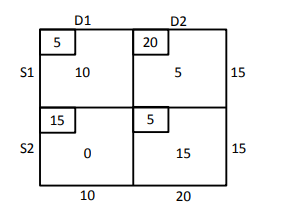
\includegraphics[width=0.75\columnwidth]{chapters/10/7/2/4/figs/fig.png}
 \end{center}
\caption{}
\label{fig:10/7/2/4Fig1}
\end{figure}
\fi

\item Find the position vector of the mid point of the vector joining the points $\vec{P}$(2, 3, 4)
and $\vec{Q}$(4, 1, –2).
\\
\solution
		\begin{enumerate}[label=\thesubsection.\arabic*,ref=\thesubsection.\theenumi]
\item Find the coordinates of the point which divides the join of $(-1,7) $ and $ (4,-3)$ in the ratio 2:3.
	\\
		\solution
	\input{chapters/10/7/2/1/section.tex}
\item Find the coordinates of the point $\vec{R}$ on the line segment joining the points $\vec{P}(-1,3)$ and $\vec{Q}(2,5)$ such that $PR=\frac{3}{5}PQ$.
\item Find the ratio in which the point $\vec{P}\brak{\frac{3}{4},\frac{5}{12}}$ divides the line segment joining the points $\vec{A}\brak{\frac{1}{2},\frac{3}{2}}$ and $ \vec{B}(2,-5)$.
\item Find the coordinates of the point which divides the line segment joining the points $(4,-3)$ and $(8,5)$ in the ratio $3:1$ internally.
\item Find the coordinates of the point $\vec{P}$ on $AD$ such that $AP : PD = 2 : 1$.
\item If the point $\vec{P} (2, 1)$ lies on the line segment joining points $\vec{A} (4, 2)$  and $ \vec{B} (8, 4)$,
then
\begin{enumerate}
	\item $AP =\frac{1}{3}{AB}$ 
\item ${AP}={PE}$
\item ${PB}=\frac{1}{3}{AB}$
\item${AP}=\frac{1}{2}{AB}$
 \end{enumerate}
\item Find the ratio in which the line segment joining the points $(-3,10)$  and  $(6,-8)$  is divided by $ (-1,6)$.
	\\
		\solution
	\input{chapters/10/7/2/4/section.tex}
\item Find the position vector of the mid point of the vector joining the points $\vec{P}$(2, 3, 4)
and $\vec{Q}$(4, 1, –2).
\\
\solution
		\input{chapters/12/10/2/16/section.tex}
\item Let $\vec{A}(4, 2), \vec{B}(6, 5)$  and $ \vec{C}(1, 4)$ be the vertices of $\triangle ABC$.
\begin{enumerate}
\item If $\vec{A}$ and  $\vec{B}$ are $(-2,-2)$ and  $(2,-4)$, respectively, find the coordinates of $\vec{P}$ such that $AP= \frac {3}{7}AB$  and $ \vec{P}$ lies on the line segment $AB$.
	\\
		\solution
	\input{chapters/10/7/2/8/section.tex}
\item Find the coordinates of the points which divide the line segment joining $A(-2,2)$  and  $\vec{B}(2,8)$ into four equal parts.
	\\
		\solution
	\input{chapters/10/7/2/9/section.tex}
\item In what ratio does the point $(-4,6)$ divide the line segment joining the points $\vec{A}(-6,0)$ and $\vec{B}(3,-8)$?
\item Given that $\vec{P}(3,2,-4), \vec{Q}(5,4,-6)$ and $\vec{R}(9,8,-10)$ are collinear. Find the ratio in which $\vec{Q}$ divides $PR$.
\item Points $\vec{A}(-6,10),\vec{B}(-4,6)$  and  $\vec{C}(3,-8)$ are collinear such that $AB=  \frac{2}{9}AC$.
\item The point which divides the line segment joining the points $\vec{P} (7, –6) $  and  $\vec{Q}(3, 4)$ in the 
ratio 1 : 2 internally lies in  which quadrant?
\item Find the coordinates of the points of trisection of the line segment joining $(4,-1)$  and  $(-2,3)$.
	\\
		\solution
	\input{chapters/10/7/2/2/section.tex}
\item Find the coordinates of the points which trisect the line segment joining the points $\vec{P}(4,2,-6)$ and $\vec{Q}(10,-16,6)$.
\item Find the coordinates of the points of trisection (i.e. points dividing to three equal parts) of the line segment joining the points $\vec{A}(2,-2)$ and $\vec{B}(-7,4)$.
\item Point $\vec{P}(5,-3)$ is one of the two points of trisection of line segment joining the points $\vec{A}(7,-2)$ and $\vec{B}(1,-5)$
\item Find the position vector of a point $\vec{R}$ which divides the line joining two points $\vec{P}$
and $\vec{Q}$ whose position vectors are $\hat{i}+2\hat{j}-\hat{k}$ and $-\hat{i}+\hat{j}+\hat{k}$ respectively, in the
ratio 2 : 1
\begin{enumerate}
    \item  internally
    \item  externally
\end{enumerate}
%\solution
%		\input{chapters/12/10/2/15/section.tex}
\item Find the coordinates of the point which divides the line segment joining the points which divides the line segment joining  the points $(-2,3,5)$ and $(1,-4,6)$ in the ratio 
\begin{enumerate}
\item $2:3$ internally,
\item $2:3$ externally
\end{enumerate}
\item Find the coordinates of the point which divides the line segment joining the points $(1,-2,3)$ and $(3,4,-5)$ in the ratio $2:3$
\begin{enumerate}
\item internally, and
\item externally
\end{enumerate}
\item Consider two points $\vec{P}$ and $\vec{Q}$ with position vectors $\overrightarrow{OP} = 3\overrightarrow{a}-2\overrightarrow{b}$ and $\overrightarrow{OQ}=\overrightarrow{a}+\overrightarrow{b}$. Find the position vector of a point $\vec{R}$ which divides the line joining $\vec{P}$ and $\vec{Q}$ in the ratio $2:1$, 
\begin{enumerate}
\item internally, and 
\item externally.
\end{enumerate}
\item The median from $\vec{A}$ meets $BC$ at $\vec{D}$. Find the coordinates of the point $\vec{D}$.
\item Find the coordinates of points $\vec{Q}$ and $\vec{R}$ on medians $BE$ and $CF$ respectively such that $BQ : QE = 2 : 1$  and  $CR : RF = 2 : 1$.
\item What do you observe?
\item If $\vec{A}, \vec{B}$ and $\vec{C}$  are the vertices of $\triangle ABC$, find the coordinates of the centroid of the triangle.
\end{enumerate}
\solution
	\input{chapters/10/7/4/7/section.tex}
\item If $\vec{P}(9a-2,-b)$ divides line segment joining $\vec{A}(3a+1,-3)$ and $\vec{B}(8a,5)$ in the ratio 3:1, find the values of $a$ and $b$.
\item Find the position vector of a point $\vec{R}$ which divides the line joining two points $\vec{P}$ and $\vec{Q}$ whose position vectors are $2\vec{a}+\vec{b}$ and $\vec{a}-3\vec{b}$ externally in the ratio $1:2$.
\item The position vector of the point which divides the join of points 2$\vec{a}$-3$\vec{b}$ $\text{and}$ $\vec{a}+\vec{b}$ in the ratio 3:1 is \rule{1cm}{0.1pt}.
\item If $\vec{a}$ and $\vec{b}$ are the postion vectors of $\vec{A}$ and $\vec{B}$, respectively, find the position vector of a point $\vec{C}$ in $BA$ produced such that $BC=1.5BA$.
\item Find the position vector of a point $\vec{R}$ which divides the line joining two points $\vec{P}$ and $\vec{Q}$ whose position vectors are $(2\vec{a}+\vec{b})$ and $(\vec{a}-3\vec{b})$
externally in the ratio 1 : 2. Also, show that $\vec{P}$ is the mid point of the line segment $RQ$.
\end{enumerate}

\item Let $\vec{A}(4, 2), \vec{B}(6, 5)$  and $ \vec{C}(1, 4)$ be the vertices of $\triangle ABC$.
\begin{enumerate}
\item If $\vec{A}$ and  $\vec{B}$ are $(-2,-2)$ and  $(2,-4)$, respectively, find the coordinates of $\vec{P}$ such that $AP= \frac {3}{7}AB$  and $ \vec{P}$ lies on the line segment $AB$.
	\\
		\solution
	\begin{enumerate}[label=\thesubsection.\arabic*,ref=\thesubsection.\theenumi]
\item Find the coordinates of the point which divides the join of $(-1,7) $ and $ (4,-3)$ in the ratio 2:3.
	\\
		\solution
	\input{chapters/10/7/2/1/section.tex}
\item Find the coordinates of the point $\vec{R}$ on the line segment joining the points $\vec{P}(-1,3)$ and $\vec{Q}(2,5)$ such that $PR=\frac{3}{5}PQ$.
\item Find the ratio in which the point $\vec{P}\brak{\frac{3}{4},\frac{5}{12}}$ divides the line segment joining the points $\vec{A}\brak{\frac{1}{2},\frac{3}{2}}$ and $ \vec{B}(2,-5)$.
\item Find the coordinates of the point which divides the line segment joining the points $(4,-3)$ and $(8,5)$ in the ratio $3:1$ internally.
\item Find the coordinates of the point $\vec{P}$ on $AD$ such that $AP : PD = 2 : 1$.
\item If the point $\vec{P} (2, 1)$ lies on the line segment joining points $\vec{A} (4, 2)$  and $ \vec{B} (8, 4)$,
then
\begin{enumerate}
	\item $AP =\frac{1}{3}{AB}$ 
\item ${AP}={PE}$
\item ${PB}=\frac{1}{3}{AB}$
\item${AP}=\frac{1}{2}{AB}$
 \end{enumerate}
\item Find the ratio in which the line segment joining the points $(-3,10)$  and  $(6,-8)$  is divided by $ (-1,6)$.
	\\
		\solution
	\input{chapters/10/7/2/4/section.tex}
\item Find the position vector of the mid point of the vector joining the points $\vec{P}$(2, 3, 4)
and $\vec{Q}$(4, 1, –2).
\\
\solution
		\input{chapters/12/10/2/16/section.tex}
\item Let $\vec{A}(4, 2), \vec{B}(6, 5)$  and $ \vec{C}(1, 4)$ be the vertices of $\triangle ABC$.
\begin{enumerate}
\item If $\vec{A}$ and  $\vec{B}$ are $(-2,-2)$ and  $(2,-4)$, respectively, find the coordinates of $\vec{P}$ such that $AP= \frac {3}{7}AB$  and $ \vec{P}$ lies on the line segment $AB$.
	\\
		\solution
	\input{chapters/10/7/2/8/section.tex}
\item Find the coordinates of the points which divide the line segment joining $A(-2,2)$  and  $\vec{B}(2,8)$ into four equal parts.
	\\
		\solution
	\input{chapters/10/7/2/9/section.tex}
\item In what ratio does the point $(-4,6)$ divide the line segment joining the points $\vec{A}(-6,0)$ and $\vec{B}(3,-8)$?
\item Given that $\vec{P}(3,2,-4), \vec{Q}(5,4,-6)$ and $\vec{R}(9,8,-10)$ are collinear. Find the ratio in which $\vec{Q}$ divides $PR$.
\item Points $\vec{A}(-6,10),\vec{B}(-4,6)$  and  $\vec{C}(3,-8)$ are collinear such that $AB=  \frac{2}{9}AC$.
\item The point which divides the line segment joining the points $\vec{P} (7, –6) $  and  $\vec{Q}(3, 4)$ in the 
ratio 1 : 2 internally lies in  which quadrant?
\item Find the coordinates of the points of trisection of the line segment joining $(4,-1)$  and  $(-2,3)$.
	\\
		\solution
	\input{chapters/10/7/2/2/section.tex}
\item Find the coordinates of the points which trisect the line segment joining the points $\vec{P}(4,2,-6)$ and $\vec{Q}(10,-16,6)$.
\item Find the coordinates of the points of trisection (i.e. points dividing to three equal parts) of the line segment joining the points $\vec{A}(2,-2)$ and $\vec{B}(-7,4)$.
\item Point $\vec{P}(5,-3)$ is one of the two points of trisection of line segment joining the points $\vec{A}(7,-2)$ and $\vec{B}(1,-5)$
\item Find the position vector of a point $\vec{R}$ which divides the line joining two points $\vec{P}$
and $\vec{Q}$ whose position vectors are $\hat{i}+2\hat{j}-\hat{k}$ and $-\hat{i}+\hat{j}+\hat{k}$ respectively, in the
ratio 2 : 1
\begin{enumerate}
    \item  internally
    \item  externally
\end{enumerate}
%\solution
%		\input{chapters/12/10/2/15/section.tex}
\item Find the coordinates of the point which divides the line segment joining the points which divides the line segment joining  the points $(-2,3,5)$ and $(1,-4,6)$ in the ratio 
\begin{enumerate}
\item $2:3$ internally,
\item $2:3$ externally
\end{enumerate}
\item Find the coordinates of the point which divides the line segment joining the points $(1,-2,3)$ and $(3,4,-5)$ in the ratio $2:3$
\begin{enumerate}
\item internally, and
\item externally
\end{enumerate}
\item Consider two points $\vec{P}$ and $\vec{Q}$ with position vectors $\overrightarrow{OP} = 3\overrightarrow{a}-2\overrightarrow{b}$ and $\overrightarrow{OQ}=\overrightarrow{a}+\overrightarrow{b}$. Find the position vector of a point $\vec{R}$ which divides the line joining $\vec{P}$ and $\vec{Q}$ in the ratio $2:1$, 
\begin{enumerate}
\item internally, and 
\item externally.
\end{enumerate}
\item The median from $\vec{A}$ meets $BC$ at $\vec{D}$. Find the coordinates of the point $\vec{D}$.
\item Find the coordinates of points $\vec{Q}$ and $\vec{R}$ on medians $BE$ and $CF$ respectively such that $BQ : QE = 2 : 1$  and  $CR : RF = 2 : 1$.
\item What do you observe?
\item If $\vec{A}, \vec{B}$ and $\vec{C}$  are the vertices of $\triangle ABC$, find the coordinates of the centroid of the triangle.
\end{enumerate}
\solution
	\input{chapters/10/7/4/7/section.tex}
\item If $\vec{P}(9a-2,-b)$ divides line segment joining $\vec{A}(3a+1,-3)$ and $\vec{B}(8a,5)$ in the ratio 3:1, find the values of $a$ and $b$.
\item Find the position vector of a point $\vec{R}$ which divides the line joining two points $\vec{P}$ and $\vec{Q}$ whose position vectors are $2\vec{a}+\vec{b}$ and $\vec{a}-3\vec{b}$ externally in the ratio $1:2$.
\item The position vector of the point which divides the join of points 2$\vec{a}$-3$\vec{b}$ $\text{and}$ $\vec{a}+\vec{b}$ in the ratio 3:1 is \rule{1cm}{0.1pt}.
\item If $\vec{a}$ and $\vec{b}$ are the postion vectors of $\vec{A}$ and $\vec{B}$, respectively, find the position vector of a point $\vec{C}$ in $BA$ produced such that $BC=1.5BA$.
\item Find the position vector of a point $\vec{R}$ which divides the line joining two points $\vec{P}$ and $\vec{Q}$ whose position vectors are $(2\vec{a}+\vec{b})$ and $(\vec{a}-3\vec{b})$
externally in the ratio 1 : 2. Also, show that $\vec{P}$ is the mid point of the line segment $RQ$.
\end{enumerate}

\item Find the coordinates of the points which divide the line segment joining $A(-2,2)$  and  $\vec{B}(2,8)$ into four equal parts.
	\\
		\solution
	\begin{enumerate}[label=\thesubsection.\arabic*,ref=\thesubsection.\theenumi]
\item Find the coordinates of the point which divides the join of $(-1,7) $ and $ (4,-3)$ in the ratio 2:3.
	\\
		\solution
	\input{chapters/10/7/2/1/section.tex}
\item Find the coordinates of the point $\vec{R}$ on the line segment joining the points $\vec{P}(-1,3)$ and $\vec{Q}(2,5)$ such that $PR=\frac{3}{5}PQ$.
\item Find the ratio in which the point $\vec{P}\brak{\frac{3}{4},\frac{5}{12}}$ divides the line segment joining the points $\vec{A}\brak{\frac{1}{2},\frac{3}{2}}$ and $ \vec{B}(2,-5)$.
\item Find the coordinates of the point which divides the line segment joining the points $(4,-3)$ and $(8,5)$ in the ratio $3:1$ internally.
\item Find the coordinates of the point $\vec{P}$ on $AD$ such that $AP : PD = 2 : 1$.
\item If the point $\vec{P} (2, 1)$ lies on the line segment joining points $\vec{A} (4, 2)$  and $ \vec{B} (8, 4)$,
then
\begin{enumerate}
	\item $AP =\frac{1}{3}{AB}$ 
\item ${AP}={PE}$
\item ${PB}=\frac{1}{3}{AB}$
\item${AP}=\frac{1}{2}{AB}$
 \end{enumerate}
\item Find the ratio in which the line segment joining the points $(-3,10)$  and  $(6,-8)$  is divided by $ (-1,6)$.
	\\
		\solution
	\input{chapters/10/7/2/4/section.tex}
\item Find the position vector of the mid point of the vector joining the points $\vec{P}$(2, 3, 4)
and $\vec{Q}$(4, 1, –2).
\\
\solution
		\input{chapters/12/10/2/16/section.tex}
\item Let $\vec{A}(4, 2), \vec{B}(6, 5)$  and $ \vec{C}(1, 4)$ be the vertices of $\triangle ABC$.
\begin{enumerate}
\item If $\vec{A}$ and  $\vec{B}$ are $(-2,-2)$ and  $(2,-4)$, respectively, find the coordinates of $\vec{P}$ such that $AP= \frac {3}{7}AB$  and $ \vec{P}$ lies on the line segment $AB$.
	\\
		\solution
	\input{chapters/10/7/2/8/section.tex}
\item Find the coordinates of the points which divide the line segment joining $A(-2,2)$  and  $\vec{B}(2,8)$ into four equal parts.
	\\
		\solution
	\input{chapters/10/7/2/9/section.tex}
\item In what ratio does the point $(-4,6)$ divide the line segment joining the points $\vec{A}(-6,0)$ and $\vec{B}(3,-8)$?
\item Given that $\vec{P}(3,2,-4), \vec{Q}(5,4,-6)$ and $\vec{R}(9,8,-10)$ are collinear. Find the ratio in which $\vec{Q}$ divides $PR$.
\item Points $\vec{A}(-6,10),\vec{B}(-4,6)$  and  $\vec{C}(3,-8)$ are collinear such that $AB=  \frac{2}{9}AC$.
\item The point which divides the line segment joining the points $\vec{P} (7, –6) $  and  $\vec{Q}(3, 4)$ in the 
ratio 1 : 2 internally lies in  which quadrant?
\item Find the coordinates of the points of trisection of the line segment joining $(4,-1)$  and  $(-2,3)$.
	\\
		\solution
	\input{chapters/10/7/2/2/section.tex}
\item Find the coordinates of the points which trisect the line segment joining the points $\vec{P}(4,2,-6)$ and $\vec{Q}(10,-16,6)$.
\item Find the coordinates of the points of trisection (i.e. points dividing to three equal parts) of the line segment joining the points $\vec{A}(2,-2)$ and $\vec{B}(-7,4)$.
\item Point $\vec{P}(5,-3)$ is one of the two points of trisection of line segment joining the points $\vec{A}(7,-2)$ and $\vec{B}(1,-5)$
\item Find the position vector of a point $\vec{R}$ which divides the line joining two points $\vec{P}$
and $\vec{Q}$ whose position vectors are $\hat{i}+2\hat{j}-\hat{k}$ and $-\hat{i}+\hat{j}+\hat{k}$ respectively, in the
ratio 2 : 1
\begin{enumerate}
    \item  internally
    \item  externally
\end{enumerate}
%\solution
%		\input{chapters/12/10/2/15/section.tex}
\item Find the coordinates of the point which divides the line segment joining the points which divides the line segment joining  the points $(-2,3,5)$ and $(1,-4,6)$ in the ratio 
\begin{enumerate}
\item $2:3$ internally,
\item $2:3$ externally
\end{enumerate}
\item Find the coordinates of the point which divides the line segment joining the points $(1,-2,3)$ and $(3,4,-5)$ in the ratio $2:3$
\begin{enumerate}
\item internally, and
\item externally
\end{enumerate}
\item Consider two points $\vec{P}$ and $\vec{Q}$ with position vectors $\overrightarrow{OP} = 3\overrightarrow{a}-2\overrightarrow{b}$ and $\overrightarrow{OQ}=\overrightarrow{a}+\overrightarrow{b}$. Find the position vector of a point $\vec{R}$ which divides the line joining $\vec{P}$ and $\vec{Q}$ in the ratio $2:1$, 
\begin{enumerate}
\item internally, and 
\item externally.
\end{enumerate}
\item The median from $\vec{A}$ meets $BC$ at $\vec{D}$. Find the coordinates of the point $\vec{D}$.
\item Find the coordinates of points $\vec{Q}$ and $\vec{R}$ on medians $BE$ and $CF$ respectively such that $BQ : QE = 2 : 1$  and  $CR : RF = 2 : 1$.
\item What do you observe?
\item If $\vec{A}, \vec{B}$ and $\vec{C}$  are the vertices of $\triangle ABC$, find the coordinates of the centroid of the triangle.
\end{enumerate}
\solution
	\input{chapters/10/7/4/7/section.tex}
\item If $\vec{P}(9a-2,-b)$ divides line segment joining $\vec{A}(3a+1,-3)$ and $\vec{B}(8a,5)$ in the ratio 3:1, find the values of $a$ and $b$.
\item Find the position vector of a point $\vec{R}$ which divides the line joining two points $\vec{P}$ and $\vec{Q}$ whose position vectors are $2\vec{a}+\vec{b}$ and $\vec{a}-3\vec{b}$ externally in the ratio $1:2$.
\item The position vector of the point which divides the join of points 2$\vec{a}$-3$\vec{b}$ $\text{and}$ $\vec{a}+\vec{b}$ in the ratio 3:1 is \rule{1cm}{0.1pt}.
\item If $\vec{a}$ and $\vec{b}$ are the postion vectors of $\vec{A}$ and $\vec{B}$, respectively, find the position vector of a point $\vec{C}$ in $BA$ produced such that $BC=1.5BA$.
\item Find the position vector of a point $\vec{R}$ which divides the line joining two points $\vec{P}$ and $\vec{Q}$ whose position vectors are $(2\vec{a}+\vec{b})$ and $(\vec{a}-3\vec{b})$
externally in the ratio 1 : 2. Also, show that $\vec{P}$ is the mid point of the line segment $RQ$.
\end{enumerate}

\item In what ratio does the point $(-4,6)$ divide the line segment joining the points $\vec{A}(-6,0)$ and $\vec{B}(3,-8)$?
\item Given that $\vec{P}(3,2,-4), \vec{Q}(5,4,-6)$ and $\vec{R}(9,8,-10)$ are collinear. Find the ratio in which $\vec{Q}$ divides $PR$.
\item Points $\vec{A}(-6,10),\vec{B}(-4,6)$  and  $\vec{C}(3,-8)$ are collinear such that $AB=  \frac{2}{9}AC$.
\item The point which divides the line segment joining the points $\vec{P} (7, –6) $  and  $\vec{Q}(3, 4)$ in the 
ratio 1 : 2 internally lies in  which quadrant?
\item Find the coordinates of the points of trisection of the line segment joining $(4,-1)$  and  $(-2,3)$.
	\\
		\solution
	Using section formula,
\begin{align}
\vec{R}=\frac{1}{1+\frac{1}{2}}\brak{\myvec{4\\-1}+\frac{1}{2}\myvec{-2\\3}}
=\myvec{2\\ \frac{1}{3}}\\
\vec{S}=\frac{1}{1+\frac{2}{1}}\brak{\myvec{4\\-1}+\frac{2}{1}\myvec{-2\\3}}
=\myvec{0\\ \frac{5}{3}}
\end{align}
which are the desired points of trisection.
\iffalse
See
		\figref{fig:chapters/10/7/2/2/Figure}
\begin{figure}[H]
\centering
\includegraphics[width=0.75\columnwidth]{chapters/10/7/2/2/figs/dj.pdf}
\caption{}
		\label{fig:chapters/10/7/2/2/Figure}
\end{figure}
\fi

\item Find the coordinates of the points which trisect the line segment joining the points $\vec{P}(4,2,-6)$ and $\vec{Q}(10,-16,6)$.
\item Find the coordinates of the points of trisection (i.e. points dividing to three equal parts) of the line segment joining the points $\vec{A}(2,-2)$ and $\vec{B}(-7,4)$.
\item Point $\vec{P}(5,-3)$ is one of the two points of trisection of line segment joining the points $\vec{A}(7,-2)$ and $\vec{B}(1,-5)$
\item Find the position vector of a point $\vec{R}$ which divides the line joining two points $\vec{P}$
and $\vec{Q}$ whose position vectors are $\hat{i}+2\hat{j}-\hat{k}$ and $-\hat{i}+\hat{j}+\hat{k}$ respectively, in the
ratio 2 : 1
\begin{enumerate}
    \item  internally
    \item  externally
\end{enumerate}
%\solution
%		\begin{enumerate}[label=\thesubsection.\arabic*,ref=\thesubsection.\theenumi]
\item Find the coordinates of the point which divides the join of $(-1,7) $ and $ (4,-3)$ in the ratio 2:3.
	\\
		\solution
	\input{chapters/10/7/2/1/section.tex}
\item Find the coordinates of the point $\vec{R}$ on the line segment joining the points $\vec{P}(-1,3)$ and $\vec{Q}(2,5)$ such that $PR=\frac{3}{5}PQ$.
\item Find the ratio in which the point $\vec{P}\brak{\frac{3}{4},\frac{5}{12}}$ divides the line segment joining the points $\vec{A}\brak{\frac{1}{2},\frac{3}{2}}$ and $ \vec{B}(2,-5)$.
\item Find the coordinates of the point which divides the line segment joining the points $(4,-3)$ and $(8,5)$ in the ratio $3:1$ internally.
\item Find the coordinates of the point $\vec{P}$ on $AD$ such that $AP : PD = 2 : 1$.
\item If the point $\vec{P} (2, 1)$ lies on the line segment joining points $\vec{A} (4, 2)$  and $ \vec{B} (8, 4)$,
then
\begin{enumerate}
	\item $AP =\frac{1}{3}{AB}$ 
\item ${AP}={PE}$
\item ${PB}=\frac{1}{3}{AB}$
\item${AP}=\frac{1}{2}{AB}$
 \end{enumerate}
\item Find the ratio in which the line segment joining the points $(-3,10)$  and  $(6,-8)$  is divided by $ (-1,6)$.
	\\
		\solution
	\input{chapters/10/7/2/4/section.tex}
\item Find the position vector of the mid point of the vector joining the points $\vec{P}$(2, 3, 4)
and $\vec{Q}$(4, 1, –2).
\\
\solution
		\input{chapters/12/10/2/16/section.tex}
\item Let $\vec{A}(4, 2), \vec{B}(6, 5)$  and $ \vec{C}(1, 4)$ be the vertices of $\triangle ABC$.
\begin{enumerate}
\item If $\vec{A}$ and  $\vec{B}$ are $(-2,-2)$ and  $(2,-4)$, respectively, find the coordinates of $\vec{P}$ such that $AP= \frac {3}{7}AB$  and $ \vec{P}$ lies on the line segment $AB$.
	\\
		\solution
	\input{chapters/10/7/2/8/section.tex}
\item Find the coordinates of the points which divide the line segment joining $A(-2,2)$  and  $\vec{B}(2,8)$ into four equal parts.
	\\
		\solution
	\input{chapters/10/7/2/9/section.tex}
\item In what ratio does the point $(-4,6)$ divide the line segment joining the points $\vec{A}(-6,0)$ and $\vec{B}(3,-8)$?
\item Given that $\vec{P}(3,2,-4), \vec{Q}(5,4,-6)$ and $\vec{R}(9,8,-10)$ are collinear. Find the ratio in which $\vec{Q}$ divides $PR$.
\item Points $\vec{A}(-6,10),\vec{B}(-4,6)$  and  $\vec{C}(3,-8)$ are collinear such that $AB=  \frac{2}{9}AC$.
\item The point which divides the line segment joining the points $\vec{P} (7, –6) $  and  $\vec{Q}(3, 4)$ in the 
ratio 1 : 2 internally lies in  which quadrant?
\item Find the coordinates of the points of trisection of the line segment joining $(4,-1)$  and  $(-2,3)$.
	\\
		\solution
	\input{chapters/10/7/2/2/section.tex}
\item Find the coordinates of the points which trisect the line segment joining the points $\vec{P}(4,2,-6)$ and $\vec{Q}(10,-16,6)$.
\item Find the coordinates of the points of trisection (i.e. points dividing to three equal parts) of the line segment joining the points $\vec{A}(2,-2)$ and $\vec{B}(-7,4)$.
\item Point $\vec{P}(5,-3)$ is one of the two points of trisection of line segment joining the points $\vec{A}(7,-2)$ and $\vec{B}(1,-5)$
\item Find the position vector of a point $\vec{R}$ which divides the line joining two points $\vec{P}$
and $\vec{Q}$ whose position vectors are $\hat{i}+2\hat{j}-\hat{k}$ and $-\hat{i}+\hat{j}+\hat{k}$ respectively, in the
ratio 2 : 1
\begin{enumerate}
    \item  internally
    \item  externally
\end{enumerate}
%\solution
%		\input{chapters/12/10/2/15/section.tex}
\item Find the coordinates of the point which divides the line segment joining the points which divides the line segment joining  the points $(-2,3,5)$ and $(1,-4,6)$ in the ratio 
\begin{enumerate}
\item $2:3$ internally,
\item $2:3$ externally
\end{enumerate}
\item Find the coordinates of the point which divides the line segment joining the points $(1,-2,3)$ and $(3,4,-5)$ in the ratio $2:3$
\begin{enumerate}
\item internally, and
\item externally
\end{enumerate}
\item Consider two points $\vec{P}$ and $\vec{Q}$ with position vectors $\overrightarrow{OP} = 3\overrightarrow{a}-2\overrightarrow{b}$ and $\overrightarrow{OQ}=\overrightarrow{a}+\overrightarrow{b}$. Find the position vector of a point $\vec{R}$ which divides the line joining $\vec{P}$ and $\vec{Q}$ in the ratio $2:1$, 
\begin{enumerate}
\item internally, and 
\item externally.
\end{enumerate}
\item The median from $\vec{A}$ meets $BC$ at $\vec{D}$. Find the coordinates of the point $\vec{D}$.
\item Find the coordinates of points $\vec{Q}$ and $\vec{R}$ on medians $BE$ and $CF$ respectively such that $BQ : QE = 2 : 1$  and  $CR : RF = 2 : 1$.
\item What do you observe?
\item If $\vec{A}, \vec{B}$ and $\vec{C}$  are the vertices of $\triangle ABC$, find the coordinates of the centroid of the triangle.
\end{enumerate}
\solution
	\input{chapters/10/7/4/7/section.tex}
\item If $\vec{P}(9a-2,-b)$ divides line segment joining $\vec{A}(3a+1,-3)$ and $\vec{B}(8a,5)$ in the ratio 3:1, find the values of $a$ and $b$.
\item Find the position vector of a point $\vec{R}$ which divides the line joining two points $\vec{P}$ and $\vec{Q}$ whose position vectors are $2\vec{a}+\vec{b}$ and $\vec{a}-3\vec{b}$ externally in the ratio $1:2$.
\item The position vector of the point which divides the join of points 2$\vec{a}$-3$\vec{b}$ $\text{and}$ $\vec{a}+\vec{b}$ in the ratio 3:1 is \rule{1cm}{0.1pt}.
\item If $\vec{a}$ and $\vec{b}$ are the postion vectors of $\vec{A}$ and $\vec{B}$, respectively, find the position vector of a point $\vec{C}$ in $BA$ produced such that $BC=1.5BA$.
\item Find the position vector of a point $\vec{R}$ which divides the line joining two points $\vec{P}$ and $\vec{Q}$ whose position vectors are $(2\vec{a}+\vec{b})$ and $(\vec{a}-3\vec{b})$
externally in the ratio 1 : 2. Also, show that $\vec{P}$ is the mid point of the line segment $RQ$.
\end{enumerate}

\item Find the coordinates of the point which divides the line segment joining the points which divides the line segment joining  the points $(-2,3,5)$ and $(1,-4,6)$ in the ratio 
\begin{enumerate}
\item $2:3$ internally,
\item $2:3$ externally
\end{enumerate}
\item Find the coordinates of the point which divides the line segment joining the points $(1,-2,3)$ and $(3,4,-5)$ in the ratio $2:3$
\begin{enumerate}
\item internally, and
\item externally
\end{enumerate}
\item Consider two points $\vec{P}$ and $\vec{Q}$ with position vectors $\overrightarrow{OP} = 3\overrightarrow{a}-2\overrightarrow{b}$ and $\overrightarrow{OQ}=\overrightarrow{a}+\overrightarrow{b}$. Find the position vector of a point $\vec{R}$ which divides the line joining $\vec{P}$ and $\vec{Q}$ in the ratio $2:1$, 
\begin{enumerate}
\item internally, and 
\item externally.
\end{enumerate}
\item The median from $\vec{A}$ meets $BC$ at $\vec{D}$. Find the coordinates of the point $\vec{D}$.
\item Find the coordinates of points $\vec{Q}$ and $\vec{R}$ on medians $BE$ and $CF$ respectively such that $BQ : QE = 2 : 1$  and  $CR : RF = 2 : 1$.
\item What do you observe?
\item If $\vec{A}, \vec{B}$ and $\vec{C}$  are the vertices of $\triangle ABC$, find the coordinates of the centroid of the triangle.
\end{enumerate}
\solution
	\begin{enumerate}[label=\thesubsection.\arabic*,ref=\thesubsection.\theenumi]
\item Find the coordinates of the point which divides the join of $(-1,7) $ and $ (4,-3)$ in the ratio 2:3.
	\\
		\solution
	\input{chapters/10/7/2/1/section.tex}
\item Find the coordinates of the point $\vec{R}$ on the line segment joining the points $\vec{P}(-1,3)$ and $\vec{Q}(2,5)$ such that $PR=\frac{3}{5}PQ$.
\item Find the ratio in which the point $\vec{P}\brak{\frac{3}{4},\frac{5}{12}}$ divides the line segment joining the points $\vec{A}\brak{\frac{1}{2},\frac{3}{2}}$ and $ \vec{B}(2,-5)$.
\item Find the coordinates of the point which divides the line segment joining the points $(4,-3)$ and $(8,5)$ in the ratio $3:1$ internally.
\item Find the coordinates of the point $\vec{P}$ on $AD$ such that $AP : PD = 2 : 1$.
\item If the point $\vec{P} (2, 1)$ lies on the line segment joining points $\vec{A} (4, 2)$  and $ \vec{B} (8, 4)$,
then
\begin{enumerate}
	\item $AP =\frac{1}{3}{AB}$ 
\item ${AP}={PE}$
\item ${PB}=\frac{1}{3}{AB}$
\item${AP}=\frac{1}{2}{AB}$
 \end{enumerate}
\item Find the ratio in which the line segment joining the points $(-3,10)$  and  $(6,-8)$  is divided by $ (-1,6)$.
	\\
		\solution
	\input{chapters/10/7/2/4/section.tex}
\item Find the position vector of the mid point of the vector joining the points $\vec{P}$(2, 3, 4)
and $\vec{Q}$(4, 1, –2).
\\
\solution
		\input{chapters/12/10/2/16/section.tex}
\item Let $\vec{A}(4, 2), \vec{B}(6, 5)$  and $ \vec{C}(1, 4)$ be the vertices of $\triangle ABC$.
\begin{enumerate}
\item If $\vec{A}$ and  $\vec{B}$ are $(-2,-2)$ and  $(2,-4)$, respectively, find the coordinates of $\vec{P}$ such that $AP= \frac {3}{7}AB$  and $ \vec{P}$ lies on the line segment $AB$.
	\\
		\solution
	\input{chapters/10/7/2/8/section.tex}
\item Find the coordinates of the points which divide the line segment joining $A(-2,2)$  and  $\vec{B}(2,8)$ into four equal parts.
	\\
		\solution
	\input{chapters/10/7/2/9/section.tex}
\item In what ratio does the point $(-4,6)$ divide the line segment joining the points $\vec{A}(-6,0)$ and $\vec{B}(3,-8)$?
\item Given that $\vec{P}(3,2,-4), \vec{Q}(5,4,-6)$ and $\vec{R}(9,8,-10)$ are collinear. Find the ratio in which $\vec{Q}$ divides $PR$.
\item Points $\vec{A}(-6,10),\vec{B}(-4,6)$  and  $\vec{C}(3,-8)$ are collinear such that $AB=  \frac{2}{9}AC$.
\item The point which divides the line segment joining the points $\vec{P} (7, –6) $  and  $\vec{Q}(3, 4)$ in the 
ratio 1 : 2 internally lies in  which quadrant?
\item Find the coordinates of the points of trisection of the line segment joining $(4,-1)$  and  $(-2,3)$.
	\\
		\solution
	\input{chapters/10/7/2/2/section.tex}
\item Find the coordinates of the points which trisect the line segment joining the points $\vec{P}(4,2,-6)$ and $\vec{Q}(10,-16,6)$.
\item Find the coordinates of the points of trisection (i.e. points dividing to three equal parts) of the line segment joining the points $\vec{A}(2,-2)$ and $\vec{B}(-7,4)$.
\item Point $\vec{P}(5,-3)$ is one of the two points of trisection of line segment joining the points $\vec{A}(7,-2)$ and $\vec{B}(1,-5)$
\item Find the position vector of a point $\vec{R}$ which divides the line joining two points $\vec{P}$
and $\vec{Q}$ whose position vectors are $\hat{i}+2\hat{j}-\hat{k}$ and $-\hat{i}+\hat{j}+\hat{k}$ respectively, in the
ratio 2 : 1
\begin{enumerate}
    \item  internally
    \item  externally
\end{enumerate}
%\solution
%		\input{chapters/12/10/2/15/section.tex}
\item Find the coordinates of the point which divides the line segment joining the points which divides the line segment joining  the points $(-2,3,5)$ and $(1,-4,6)$ in the ratio 
\begin{enumerate}
\item $2:3$ internally,
\item $2:3$ externally
\end{enumerate}
\item Find the coordinates of the point which divides the line segment joining the points $(1,-2,3)$ and $(3,4,-5)$ in the ratio $2:3$
\begin{enumerate}
\item internally, and
\item externally
\end{enumerate}
\item Consider two points $\vec{P}$ and $\vec{Q}$ with position vectors $\overrightarrow{OP} = 3\overrightarrow{a}-2\overrightarrow{b}$ and $\overrightarrow{OQ}=\overrightarrow{a}+\overrightarrow{b}$. Find the position vector of a point $\vec{R}$ which divides the line joining $\vec{P}$ and $\vec{Q}$ in the ratio $2:1$, 
\begin{enumerate}
\item internally, and 
\item externally.
\end{enumerate}
\item The median from $\vec{A}$ meets $BC$ at $\vec{D}$. Find the coordinates of the point $\vec{D}$.
\item Find the coordinates of points $\vec{Q}$ and $\vec{R}$ on medians $BE$ and $CF$ respectively such that $BQ : QE = 2 : 1$  and  $CR : RF = 2 : 1$.
\item What do you observe?
\item If $\vec{A}, \vec{B}$ and $\vec{C}$  are the vertices of $\triangle ABC$, find the coordinates of the centroid of the triangle.
\end{enumerate}
\solution
	\input{chapters/10/7/4/7/section.tex}
\item If $\vec{P}(9a-2,-b)$ divides line segment joining $\vec{A}(3a+1,-3)$ and $\vec{B}(8a,5)$ in the ratio 3:1, find the values of $a$ and $b$.
\item Find the position vector of a point $\vec{R}$ which divides the line joining two points $\vec{P}$ and $\vec{Q}$ whose position vectors are $2\vec{a}+\vec{b}$ and $\vec{a}-3\vec{b}$ externally in the ratio $1:2$.
\item The position vector of the point which divides the join of points 2$\vec{a}$-3$\vec{b}$ $\text{and}$ $\vec{a}+\vec{b}$ in the ratio 3:1 is \rule{1cm}{0.1pt}.
\item If $\vec{a}$ and $\vec{b}$ are the postion vectors of $\vec{A}$ and $\vec{B}$, respectively, find the position vector of a point $\vec{C}$ in $BA$ produced such that $BC=1.5BA$.
\item Find the position vector of a point $\vec{R}$ which divides the line joining two points $\vec{P}$ and $\vec{Q}$ whose position vectors are $(2\vec{a}+\vec{b})$ and $(\vec{a}-3\vec{b})$
externally in the ratio 1 : 2. Also, show that $\vec{P}$ is the mid point of the line segment $RQ$.
\end{enumerate}

\item If $\vec{P}(9a-2,-b)$ divides line segment joining $\vec{A}(3a+1,-3)$ and $\vec{B}(8a,5)$ in the ratio 3:1, find the values of $a$ and $b$.
\item Find the position vector of a point $\vec{R}$ which divides the line joining two points $\vec{P}$ and $\vec{Q}$ whose position vectors are $2\vec{a}+\vec{b}$ and $\vec{a}-3\vec{b}$ externally in the ratio $1:2$.
\item The position vector of the point which divides the join of points 2$\vec{a}$-3$\vec{b}$ $\text{and}$ $\vec{a}+\vec{b}$ in the ratio 3:1 is \rule{1cm}{0.1pt}.
\item If $\vec{a}$ and $\vec{b}$ are the postion vectors of $\vec{A}$ and $\vec{B}$, respectively, find the position vector of a point $\vec{C}$ in $BA$ produced such that $BC=1.5BA$.
\item Find the position vector of a point $\vec{R}$ which divides the line joining two points $\vec{P}$ and $\vec{Q}$ whose position vectors are $(2\vec{a}+\vec{b})$ and $(\vec{a}-3\vec{b})$
externally in the ratio 1 : 2. Also, show that $\vec{P}$ is the mid point of the line segment $RQ$.
\end{enumerate}

\item Find the coordinates of the points which divide the line segment joining $A(-2,2)$  and  $\vec{B}(2,8)$ into four equal parts.
	\\
		\solution
	\begin{enumerate}[label=\thesubsection.\arabic*,ref=\thesubsection.\theenumi]
\item Find the coordinates of the point which divides the join of $(-1,7) $ and $ (4,-3)$ in the ratio 2:3.
	\\
		\solution
	\begin{enumerate}[label=\thesubsection.\arabic*,ref=\thesubsection.\theenumi]
\item Find the coordinates of the point which divides the join of $(-1,7) $ and $ (4,-3)$ in the ratio 2:3.
	\\
		\solution
	\input{chapters/10/7/2/1/section.tex}
\item Find the coordinates of the point $\vec{R}$ on the line segment joining the points $\vec{P}(-1,3)$ and $\vec{Q}(2,5)$ such that $PR=\frac{3}{5}PQ$.
\item Find the ratio in which the point $\vec{P}\brak{\frac{3}{4},\frac{5}{12}}$ divides the line segment joining the points $\vec{A}\brak{\frac{1}{2},\frac{3}{2}}$ and $ \vec{B}(2,-5)$.
\item Find the coordinates of the point which divides the line segment joining the points $(4,-3)$ and $(8,5)$ in the ratio $3:1$ internally.
\item Find the coordinates of the point $\vec{P}$ on $AD$ such that $AP : PD = 2 : 1$.
\item If the point $\vec{P} (2, 1)$ lies on the line segment joining points $\vec{A} (4, 2)$  and $ \vec{B} (8, 4)$,
then
\begin{enumerate}
	\item $AP =\frac{1}{3}{AB}$ 
\item ${AP}={PE}$
\item ${PB}=\frac{1}{3}{AB}$
\item${AP}=\frac{1}{2}{AB}$
 \end{enumerate}
\item Find the ratio in which the line segment joining the points $(-3,10)$  and  $(6,-8)$  is divided by $ (-1,6)$.
	\\
		\solution
	\input{chapters/10/7/2/4/section.tex}
\item Find the position vector of the mid point of the vector joining the points $\vec{P}$(2, 3, 4)
and $\vec{Q}$(4, 1, –2).
\\
\solution
		\input{chapters/12/10/2/16/section.tex}
\item Let $\vec{A}(4, 2), \vec{B}(6, 5)$  and $ \vec{C}(1, 4)$ be the vertices of $\triangle ABC$.
\begin{enumerate}
\item If $\vec{A}$ and  $\vec{B}$ are $(-2,-2)$ and  $(2,-4)$, respectively, find the coordinates of $\vec{P}$ such that $AP= \frac {3}{7}AB$  and $ \vec{P}$ lies on the line segment $AB$.
	\\
		\solution
	\input{chapters/10/7/2/8/section.tex}
\item Find the coordinates of the points which divide the line segment joining $A(-2,2)$  and  $\vec{B}(2,8)$ into four equal parts.
	\\
		\solution
	\input{chapters/10/7/2/9/section.tex}
\item In what ratio does the point $(-4,6)$ divide the line segment joining the points $\vec{A}(-6,0)$ and $\vec{B}(3,-8)$?
\item Given that $\vec{P}(3,2,-4), \vec{Q}(5,4,-6)$ and $\vec{R}(9,8,-10)$ are collinear. Find the ratio in which $\vec{Q}$ divides $PR$.
\item Points $\vec{A}(-6,10),\vec{B}(-4,6)$  and  $\vec{C}(3,-8)$ are collinear such that $AB=  \frac{2}{9}AC$.
\item The point which divides the line segment joining the points $\vec{P} (7, –6) $  and  $\vec{Q}(3, 4)$ in the 
ratio 1 : 2 internally lies in  which quadrant?
\item Find the coordinates of the points of trisection of the line segment joining $(4,-1)$  and  $(-2,3)$.
	\\
		\solution
	\input{chapters/10/7/2/2/section.tex}
\item Find the coordinates of the points which trisect the line segment joining the points $\vec{P}(4,2,-6)$ and $\vec{Q}(10,-16,6)$.
\item Find the coordinates of the points of trisection (i.e. points dividing to three equal parts) of the line segment joining the points $\vec{A}(2,-2)$ and $\vec{B}(-7,4)$.
\item Point $\vec{P}(5,-3)$ is one of the two points of trisection of line segment joining the points $\vec{A}(7,-2)$ and $\vec{B}(1,-5)$
\item Find the position vector of a point $\vec{R}$ which divides the line joining two points $\vec{P}$
and $\vec{Q}$ whose position vectors are $\hat{i}+2\hat{j}-\hat{k}$ and $-\hat{i}+\hat{j}+\hat{k}$ respectively, in the
ratio 2 : 1
\begin{enumerate}
    \item  internally
    \item  externally
\end{enumerate}
%\solution
%		\input{chapters/12/10/2/15/section.tex}
\item Find the coordinates of the point which divides the line segment joining the points which divides the line segment joining  the points $(-2,3,5)$ and $(1,-4,6)$ in the ratio 
\begin{enumerate}
\item $2:3$ internally,
\item $2:3$ externally
\end{enumerate}
\item Find the coordinates of the point which divides the line segment joining the points $(1,-2,3)$ and $(3,4,-5)$ in the ratio $2:3$
\begin{enumerate}
\item internally, and
\item externally
\end{enumerate}
\item Consider two points $\vec{P}$ and $\vec{Q}$ with position vectors $\overrightarrow{OP} = 3\overrightarrow{a}-2\overrightarrow{b}$ and $\overrightarrow{OQ}=\overrightarrow{a}+\overrightarrow{b}$. Find the position vector of a point $\vec{R}$ which divides the line joining $\vec{P}$ and $\vec{Q}$ in the ratio $2:1$, 
\begin{enumerate}
\item internally, and 
\item externally.
\end{enumerate}
\item The median from $\vec{A}$ meets $BC$ at $\vec{D}$. Find the coordinates of the point $\vec{D}$.
\item Find the coordinates of points $\vec{Q}$ and $\vec{R}$ on medians $BE$ and $CF$ respectively such that $BQ : QE = 2 : 1$  and  $CR : RF = 2 : 1$.
\item What do you observe?
\item If $\vec{A}, \vec{B}$ and $\vec{C}$  are the vertices of $\triangle ABC$, find the coordinates of the centroid of the triangle.
\end{enumerate}
\solution
	\input{chapters/10/7/4/7/section.tex}
\item If $\vec{P}(9a-2,-b)$ divides line segment joining $\vec{A}(3a+1,-3)$ and $\vec{B}(8a,5)$ in the ratio 3:1, find the values of $a$ and $b$.
\item Find the position vector of a point $\vec{R}$ which divides the line joining two points $\vec{P}$ and $\vec{Q}$ whose position vectors are $2\vec{a}+\vec{b}$ and $\vec{a}-3\vec{b}$ externally in the ratio $1:2$.
\item The position vector of the point which divides the join of points 2$\vec{a}$-3$\vec{b}$ $\text{and}$ $\vec{a}+\vec{b}$ in the ratio 3:1 is \rule{1cm}{0.1pt}.
\item If $\vec{a}$ and $\vec{b}$ are the postion vectors of $\vec{A}$ and $\vec{B}$, respectively, find the position vector of a point $\vec{C}$ in $BA$ produced such that $BC=1.5BA$.
\item Find the position vector of a point $\vec{R}$ which divides the line joining two points $\vec{P}$ and $\vec{Q}$ whose position vectors are $(2\vec{a}+\vec{b})$ and $(\vec{a}-3\vec{b})$
externally in the ratio 1 : 2. Also, show that $\vec{P}$ is the mid point of the line segment $RQ$.
\end{enumerate}

\item Find the coordinates of the point $\vec{R}$ on the line segment joining the points $\vec{P}(-1,3)$ and $\vec{Q}(2,5)$ such that $PR=\frac{3}{5}PQ$.
\item Find the ratio in which the point $\vec{P}\brak{\frac{3}{4},\frac{5}{12}}$ divides the line segment joining the points $\vec{A}\brak{\frac{1}{2},\frac{3}{2}}$ and $ \vec{B}(2,-5)$.
\item Find the coordinates of the point which divides the line segment joining the points $(4,-3)$ and $(8,5)$ in the ratio $3:1$ internally.
\item Find the coordinates of the point $\vec{P}$ on $AD$ such that $AP : PD = 2 : 1$.
\item If the point $\vec{P} (2, 1)$ lies on the line segment joining points $\vec{A} (4, 2)$  and $ \vec{B} (8, 4)$,
then
\begin{enumerate}
	\item $AP =\frac{1}{3}{AB}$ 
\item ${AP}={PE}$
\item ${PB}=\frac{1}{3}{AB}$
\item${AP}=\frac{1}{2}{AB}$
 \end{enumerate}
\item Find the ratio in which the line segment joining the points $(-3,10)$  and  $(6,-8)$  is divided by $ (-1,6)$.
	\\
		\solution
	\iffalse
Using section formula,
\begin{align}
         \myvec{-1\\6} &=\frac{{\myvec{-3\\10}+k\myvec{6\\-8}}}{1+k}\\
	 \implies 7k\myvec{1 \\ -2} &= 2\myvec{1 \\ -2}
	 \\
	 \text{or, } k &= \frac{2}{7}.
\end{align}
\fi
In 
			\eqref{eq:section_formula-k}, substituting
			\begin{align}
				\vec{B} &= \myvec{-3\\10}, \vec{C} = \myvec{6\\-8}, \vec{D} = \myvec{-1\\6},
				\\
				k &= \frac{\myvec{-2 & 4}\myvec{-7 \\ 14}}{\norm{\myvec{-7 \\ 14}}^2} = \frac{2}{7}
			\end{align}
\iffalse
See \figref{fig:10/7/2/4Fig1}.
\begin{figure}[H]
 \begin{center}
  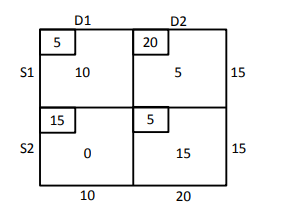
\includegraphics[width=0.75\columnwidth]{chapters/10/7/2/4/figs/fig.png}
 \end{center}
\caption{}
\label{fig:10/7/2/4Fig1}
\end{figure}
\fi

\item Find the position vector of the mid point of the vector joining the points $\vec{P}$(2, 3, 4)
and $\vec{Q}$(4, 1, –2).
\\
\solution
		\begin{enumerate}[label=\thesubsection.\arabic*,ref=\thesubsection.\theenumi]
\item Find the coordinates of the point which divides the join of $(-1,7) $ and $ (4,-3)$ in the ratio 2:3.
	\\
		\solution
	\input{chapters/10/7/2/1/section.tex}
\item Find the coordinates of the point $\vec{R}$ on the line segment joining the points $\vec{P}(-1,3)$ and $\vec{Q}(2,5)$ such that $PR=\frac{3}{5}PQ$.
\item Find the ratio in which the point $\vec{P}\brak{\frac{3}{4},\frac{5}{12}}$ divides the line segment joining the points $\vec{A}\brak{\frac{1}{2},\frac{3}{2}}$ and $ \vec{B}(2,-5)$.
\item Find the coordinates of the point which divides the line segment joining the points $(4,-3)$ and $(8,5)$ in the ratio $3:1$ internally.
\item Find the coordinates of the point $\vec{P}$ on $AD$ such that $AP : PD = 2 : 1$.
\item If the point $\vec{P} (2, 1)$ lies on the line segment joining points $\vec{A} (4, 2)$  and $ \vec{B} (8, 4)$,
then
\begin{enumerate}
	\item $AP =\frac{1}{3}{AB}$ 
\item ${AP}={PE}$
\item ${PB}=\frac{1}{3}{AB}$
\item${AP}=\frac{1}{2}{AB}$
 \end{enumerate}
\item Find the ratio in which the line segment joining the points $(-3,10)$  and  $(6,-8)$  is divided by $ (-1,6)$.
	\\
		\solution
	\input{chapters/10/7/2/4/section.tex}
\item Find the position vector of the mid point of the vector joining the points $\vec{P}$(2, 3, 4)
and $\vec{Q}$(4, 1, –2).
\\
\solution
		\input{chapters/12/10/2/16/section.tex}
\item Let $\vec{A}(4, 2), \vec{B}(6, 5)$  and $ \vec{C}(1, 4)$ be the vertices of $\triangle ABC$.
\begin{enumerate}
\item If $\vec{A}$ and  $\vec{B}$ are $(-2,-2)$ and  $(2,-4)$, respectively, find the coordinates of $\vec{P}$ such that $AP= \frac {3}{7}AB$  and $ \vec{P}$ lies on the line segment $AB$.
	\\
		\solution
	\input{chapters/10/7/2/8/section.tex}
\item Find the coordinates of the points which divide the line segment joining $A(-2,2)$  and  $\vec{B}(2,8)$ into four equal parts.
	\\
		\solution
	\input{chapters/10/7/2/9/section.tex}
\item In what ratio does the point $(-4,6)$ divide the line segment joining the points $\vec{A}(-6,0)$ and $\vec{B}(3,-8)$?
\item Given that $\vec{P}(3,2,-4), \vec{Q}(5,4,-6)$ and $\vec{R}(9,8,-10)$ are collinear. Find the ratio in which $\vec{Q}$ divides $PR$.
\item Points $\vec{A}(-6,10),\vec{B}(-4,6)$  and  $\vec{C}(3,-8)$ are collinear such that $AB=  \frac{2}{9}AC$.
\item The point which divides the line segment joining the points $\vec{P} (7, –6) $  and  $\vec{Q}(3, 4)$ in the 
ratio 1 : 2 internally lies in  which quadrant?
\item Find the coordinates of the points of trisection of the line segment joining $(4,-1)$  and  $(-2,3)$.
	\\
		\solution
	\input{chapters/10/7/2/2/section.tex}
\item Find the coordinates of the points which trisect the line segment joining the points $\vec{P}(4,2,-6)$ and $\vec{Q}(10,-16,6)$.
\item Find the coordinates of the points of trisection (i.e. points dividing to three equal parts) of the line segment joining the points $\vec{A}(2,-2)$ and $\vec{B}(-7,4)$.
\item Point $\vec{P}(5,-3)$ is one of the two points of trisection of line segment joining the points $\vec{A}(7,-2)$ and $\vec{B}(1,-5)$
\item Find the position vector of a point $\vec{R}$ which divides the line joining two points $\vec{P}$
and $\vec{Q}$ whose position vectors are $\hat{i}+2\hat{j}-\hat{k}$ and $-\hat{i}+\hat{j}+\hat{k}$ respectively, in the
ratio 2 : 1
\begin{enumerate}
    \item  internally
    \item  externally
\end{enumerate}
%\solution
%		\input{chapters/12/10/2/15/section.tex}
\item Find the coordinates of the point which divides the line segment joining the points which divides the line segment joining  the points $(-2,3,5)$ and $(1,-4,6)$ in the ratio 
\begin{enumerate}
\item $2:3$ internally,
\item $2:3$ externally
\end{enumerate}
\item Find the coordinates of the point which divides the line segment joining the points $(1,-2,3)$ and $(3,4,-5)$ in the ratio $2:3$
\begin{enumerate}
\item internally, and
\item externally
\end{enumerate}
\item Consider two points $\vec{P}$ and $\vec{Q}$ with position vectors $\overrightarrow{OP} = 3\overrightarrow{a}-2\overrightarrow{b}$ and $\overrightarrow{OQ}=\overrightarrow{a}+\overrightarrow{b}$. Find the position vector of a point $\vec{R}$ which divides the line joining $\vec{P}$ and $\vec{Q}$ in the ratio $2:1$, 
\begin{enumerate}
\item internally, and 
\item externally.
\end{enumerate}
\item The median from $\vec{A}$ meets $BC$ at $\vec{D}$. Find the coordinates of the point $\vec{D}$.
\item Find the coordinates of points $\vec{Q}$ and $\vec{R}$ on medians $BE$ and $CF$ respectively such that $BQ : QE = 2 : 1$  and  $CR : RF = 2 : 1$.
\item What do you observe?
\item If $\vec{A}, \vec{B}$ and $\vec{C}$  are the vertices of $\triangle ABC$, find the coordinates of the centroid of the triangle.
\end{enumerate}
\solution
	\input{chapters/10/7/4/7/section.tex}
\item If $\vec{P}(9a-2,-b)$ divides line segment joining $\vec{A}(3a+1,-3)$ and $\vec{B}(8a,5)$ in the ratio 3:1, find the values of $a$ and $b$.
\item Find the position vector of a point $\vec{R}$ which divides the line joining two points $\vec{P}$ and $\vec{Q}$ whose position vectors are $2\vec{a}+\vec{b}$ and $\vec{a}-3\vec{b}$ externally in the ratio $1:2$.
\item The position vector of the point which divides the join of points 2$\vec{a}$-3$\vec{b}$ $\text{and}$ $\vec{a}+\vec{b}$ in the ratio 3:1 is \rule{1cm}{0.1pt}.
\item If $\vec{a}$ and $\vec{b}$ are the postion vectors of $\vec{A}$ and $\vec{B}$, respectively, find the position vector of a point $\vec{C}$ in $BA$ produced such that $BC=1.5BA$.
\item Find the position vector of a point $\vec{R}$ which divides the line joining two points $\vec{P}$ and $\vec{Q}$ whose position vectors are $(2\vec{a}+\vec{b})$ and $(\vec{a}-3\vec{b})$
externally in the ratio 1 : 2. Also, show that $\vec{P}$ is the mid point of the line segment $RQ$.
\end{enumerate}

\item Let $\vec{A}(4, 2), \vec{B}(6, 5)$  and $ \vec{C}(1, 4)$ be the vertices of $\triangle ABC$.
\begin{enumerate}
\item If $\vec{A}$ and  $\vec{B}$ are $(-2,-2)$ and  $(2,-4)$, respectively, find the coordinates of $\vec{P}$ such that $AP= \frac {3}{7}AB$  and $ \vec{P}$ lies on the line segment $AB$.
	\\
		\solution
	\begin{enumerate}[label=\thesubsection.\arabic*,ref=\thesubsection.\theenumi]
\item Find the coordinates of the point which divides the join of $(-1,7) $ and $ (4,-3)$ in the ratio 2:3.
	\\
		\solution
	\input{chapters/10/7/2/1/section.tex}
\item Find the coordinates of the point $\vec{R}$ on the line segment joining the points $\vec{P}(-1,3)$ and $\vec{Q}(2,5)$ such that $PR=\frac{3}{5}PQ$.
\item Find the ratio in which the point $\vec{P}\brak{\frac{3}{4},\frac{5}{12}}$ divides the line segment joining the points $\vec{A}\brak{\frac{1}{2},\frac{3}{2}}$ and $ \vec{B}(2,-5)$.
\item Find the coordinates of the point which divides the line segment joining the points $(4,-3)$ and $(8,5)$ in the ratio $3:1$ internally.
\item Find the coordinates of the point $\vec{P}$ on $AD$ such that $AP : PD = 2 : 1$.
\item If the point $\vec{P} (2, 1)$ lies on the line segment joining points $\vec{A} (4, 2)$  and $ \vec{B} (8, 4)$,
then
\begin{enumerate}
	\item $AP =\frac{1}{3}{AB}$ 
\item ${AP}={PE}$
\item ${PB}=\frac{1}{3}{AB}$
\item${AP}=\frac{1}{2}{AB}$
 \end{enumerate}
\item Find the ratio in which the line segment joining the points $(-3,10)$  and  $(6,-8)$  is divided by $ (-1,6)$.
	\\
		\solution
	\input{chapters/10/7/2/4/section.tex}
\item Find the position vector of the mid point of the vector joining the points $\vec{P}$(2, 3, 4)
and $\vec{Q}$(4, 1, –2).
\\
\solution
		\input{chapters/12/10/2/16/section.tex}
\item Let $\vec{A}(4, 2), \vec{B}(6, 5)$  and $ \vec{C}(1, 4)$ be the vertices of $\triangle ABC$.
\begin{enumerate}
\item If $\vec{A}$ and  $\vec{B}$ are $(-2,-2)$ and  $(2,-4)$, respectively, find the coordinates of $\vec{P}$ such that $AP= \frac {3}{7}AB$  and $ \vec{P}$ lies on the line segment $AB$.
	\\
		\solution
	\input{chapters/10/7/2/8/section.tex}
\item Find the coordinates of the points which divide the line segment joining $A(-2,2)$  and  $\vec{B}(2,8)$ into four equal parts.
	\\
		\solution
	\input{chapters/10/7/2/9/section.tex}
\item In what ratio does the point $(-4,6)$ divide the line segment joining the points $\vec{A}(-6,0)$ and $\vec{B}(3,-8)$?
\item Given that $\vec{P}(3,2,-4), \vec{Q}(5,4,-6)$ and $\vec{R}(9,8,-10)$ are collinear. Find the ratio in which $\vec{Q}$ divides $PR$.
\item Points $\vec{A}(-6,10),\vec{B}(-4,6)$  and  $\vec{C}(3,-8)$ are collinear such that $AB=  \frac{2}{9}AC$.
\item The point which divides the line segment joining the points $\vec{P} (7, –6) $  and  $\vec{Q}(3, 4)$ in the 
ratio 1 : 2 internally lies in  which quadrant?
\item Find the coordinates of the points of trisection of the line segment joining $(4,-1)$  and  $(-2,3)$.
	\\
		\solution
	\input{chapters/10/7/2/2/section.tex}
\item Find the coordinates of the points which trisect the line segment joining the points $\vec{P}(4,2,-6)$ and $\vec{Q}(10,-16,6)$.
\item Find the coordinates of the points of trisection (i.e. points dividing to three equal parts) of the line segment joining the points $\vec{A}(2,-2)$ and $\vec{B}(-7,4)$.
\item Point $\vec{P}(5,-3)$ is one of the two points of trisection of line segment joining the points $\vec{A}(7,-2)$ and $\vec{B}(1,-5)$
\item Find the position vector of a point $\vec{R}$ which divides the line joining two points $\vec{P}$
and $\vec{Q}$ whose position vectors are $\hat{i}+2\hat{j}-\hat{k}$ and $-\hat{i}+\hat{j}+\hat{k}$ respectively, in the
ratio 2 : 1
\begin{enumerate}
    \item  internally
    \item  externally
\end{enumerate}
%\solution
%		\input{chapters/12/10/2/15/section.tex}
\item Find the coordinates of the point which divides the line segment joining the points which divides the line segment joining  the points $(-2,3,5)$ and $(1,-4,6)$ in the ratio 
\begin{enumerate}
\item $2:3$ internally,
\item $2:3$ externally
\end{enumerate}
\item Find the coordinates of the point which divides the line segment joining the points $(1,-2,3)$ and $(3,4,-5)$ in the ratio $2:3$
\begin{enumerate}
\item internally, and
\item externally
\end{enumerate}
\item Consider two points $\vec{P}$ and $\vec{Q}$ with position vectors $\overrightarrow{OP} = 3\overrightarrow{a}-2\overrightarrow{b}$ and $\overrightarrow{OQ}=\overrightarrow{a}+\overrightarrow{b}$. Find the position vector of a point $\vec{R}$ which divides the line joining $\vec{P}$ and $\vec{Q}$ in the ratio $2:1$, 
\begin{enumerate}
\item internally, and 
\item externally.
\end{enumerate}
\item The median from $\vec{A}$ meets $BC$ at $\vec{D}$. Find the coordinates of the point $\vec{D}$.
\item Find the coordinates of points $\vec{Q}$ and $\vec{R}$ on medians $BE$ and $CF$ respectively such that $BQ : QE = 2 : 1$  and  $CR : RF = 2 : 1$.
\item What do you observe?
\item If $\vec{A}, \vec{B}$ and $\vec{C}$  are the vertices of $\triangle ABC$, find the coordinates of the centroid of the triangle.
\end{enumerate}
\solution
	\input{chapters/10/7/4/7/section.tex}
\item If $\vec{P}(9a-2,-b)$ divides line segment joining $\vec{A}(3a+1,-3)$ and $\vec{B}(8a,5)$ in the ratio 3:1, find the values of $a$ and $b$.
\item Find the position vector of a point $\vec{R}$ which divides the line joining two points $\vec{P}$ and $\vec{Q}$ whose position vectors are $2\vec{a}+\vec{b}$ and $\vec{a}-3\vec{b}$ externally in the ratio $1:2$.
\item The position vector of the point which divides the join of points 2$\vec{a}$-3$\vec{b}$ $\text{and}$ $\vec{a}+\vec{b}$ in the ratio 3:1 is \rule{1cm}{0.1pt}.
\item If $\vec{a}$ and $\vec{b}$ are the postion vectors of $\vec{A}$ and $\vec{B}$, respectively, find the position vector of a point $\vec{C}$ in $BA$ produced such that $BC=1.5BA$.
\item Find the position vector of a point $\vec{R}$ which divides the line joining two points $\vec{P}$ and $\vec{Q}$ whose position vectors are $(2\vec{a}+\vec{b})$ and $(\vec{a}-3\vec{b})$
externally in the ratio 1 : 2. Also, show that $\vec{P}$ is the mid point of the line segment $RQ$.
\end{enumerate}

\item Find the coordinates of the points which divide the line segment joining $A(-2,2)$  and  $\vec{B}(2,8)$ into four equal parts.
	\\
		\solution
	\begin{enumerate}[label=\thesubsection.\arabic*,ref=\thesubsection.\theenumi]
\item Find the coordinates of the point which divides the join of $(-1,7) $ and $ (4,-3)$ in the ratio 2:3.
	\\
		\solution
	\input{chapters/10/7/2/1/section.tex}
\item Find the coordinates of the point $\vec{R}$ on the line segment joining the points $\vec{P}(-1,3)$ and $\vec{Q}(2,5)$ such that $PR=\frac{3}{5}PQ$.
\item Find the ratio in which the point $\vec{P}\brak{\frac{3}{4},\frac{5}{12}}$ divides the line segment joining the points $\vec{A}\brak{\frac{1}{2},\frac{3}{2}}$ and $ \vec{B}(2,-5)$.
\item Find the coordinates of the point which divides the line segment joining the points $(4,-3)$ and $(8,5)$ in the ratio $3:1$ internally.
\item Find the coordinates of the point $\vec{P}$ on $AD$ such that $AP : PD = 2 : 1$.
\item If the point $\vec{P} (2, 1)$ lies on the line segment joining points $\vec{A} (4, 2)$  and $ \vec{B} (8, 4)$,
then
\begin{enumerate}
	\item $AP =\frac{1}{3}{AB}$ 
\item ${AP}={PE}$
\item ${PB}=\frac{1}{3}{AB}$
\item${AP}=\frac{1}{2}{AB}$
 \end{enumerate}
\item Find the ratio in which the line segment joining the points $(-3,10)$  and  $(6,-8)$  is divided by $ (-1,6)$.
	\\
		\solution
	\input{chapters/10/7/2/4/section.tex}
\item Find the position vector of the mid point of the vector joining the points $\vec{P}$(2, 3, 4)
and $\vec{Q}$(4, 1, –2).
\\
\solution
		\input{chapters/12/10/2/16/section.tex}
\item Let $\vec{A}(4, 2), \vec{B}(6, 5)$  and $ \vec{C}(1, 4)$ be the vertices of $\triangle ABC$.
\begin{enumerate}
\item If $\vec{A}$ and  $\vec{B}$ are $(-2,-2)$ and  $(2,-4)$, respectively, find the coordinates of $\vec{P}$ such that $AP= \frac {3}{7}AB$  and $ \vec{P}$ lies on the line segment $AB$.
	\\
		\solution
	\input{chapters/10/7/2/8/section.tex}
\item Find the coordinates of the points which divide the line segment joining $A(-2,2)$  and  $\vec{B}(2,8)$ into four equal parts.
	\\
		\solution
	\input{chapters/10/7/2/9/section.tex}
\item In what ratio does the point $(-4,6)$ divide the line segment joining the points $\vec{A}(-6,0)$ and $\vec{B}(3,-8)$?
\item Given that $\vec{P}(3,2,-4), \vec{Q}(5,4,-6)$ and $\vec{R}(9,8,-10)$ are collinear. Find the ratio in which $\vec{Q}$ divides $PR$.
\item Points $\vec{A}(-6,10),\vec{B}(-4,6)$  and  $\vec{C}(3,-8)$ are collinear such that $AB=  \frac{2}{9}AC$.
\item The point which divides the line segment joining the points $\vec{P} (7, –6) $  and  $\vec{Q}(3, 4)$ in the 
ratio 1 : 2 internally lies in  which quadrant?
\item Find the coordinates of the points of trisection of the line segment joining $(4,-1)$  and  $(-2,3)$.
	\\
		\solution
	\input{chapters/10/7/2/2/section.tex}
\item Find the coordinates of the points which trisect the line segment joining the points $\vec{P}(4,2,-6)$ and $\vec{Q}(10,-16,6)$.
\item Find the coordinates of the points of trisection (i.e. points dividing to three equal parts) of the line segment joining the points $\vec{A}(2,-2)$ and $\vec{B}(-7,4)$.
\item Point $\vec{P}(5,-3)$ is one of the two points of trisection of line segment joining the points $\vec{A}(7,-2)$ and $\vec{B}(1,-5)$
\item Find the position vector of a point $\vec{R}$ which divides the line joining two points $\vec{P}$
and $\vec{Q}$ whose position vectors are $\hat{i}+2\hat{j}-\hat{k}$ and $-\hat{i}+\hat{j}+\hat{k}$ respectively, in the
ratio 2 : 1
\begin{enumerate}
    \item  internally
    \item  externally
\end{enumerate}
%\solution
%		\input{chapters/12/10/2/15/section.tex}
\item Find the coordinates of the point which divides the line segment joining the points which divides the line segment joining  the points $(-2,3,5)$ and $(1,-4,6)$ in the ratio 
\begin{enumerate}
\item $2:3$ internally,
\item $2:3$ externally
\end{enumerate}
\item Find the coordinates of the point which divides the line segment joining the points $(1,-2,3)$ and $(3,4,-5)$ in the ratio $2:3$
\begin{enumerate}
\item internally, and
\item externally
\end{enumerate}
\item Consider two points $\vec{P}$ and $\vec{Q}$ with position vectors $\overrightarrow{OP} = 3\overrightarrow{a}-2\overrightarrow{b}$ and $\overrightarrow{OQ}=\overrightarrow{a}+\overrightarrow{b}$. Find the position vector of a point $\vec{R}$ which divides the line joining $\vec{P}$ and $\vec{Q}$ in the ratio $2:1$, 
\begin{enumerate}
\item internally, and 
\item externally.
\end{enumerate}
\item The median from $\vec{A}$ meets $BC$ at $\vec{D}$. Find the coordinates of the point $\vec{D}$.
\item Find the coordinates of points $\vec{Q}$ and $\vec{R}$ on medians $BE$ and $CF$ respectively such that $BQ : QE = 2 : 1$  and  $CR : RF = 2 : 1$.
\item What do you observe?
\item If $\vec{A}, \vec{B}$ and $\vec{C}$  are the vertices of $\triangle ABC$, find the coordinates of the centroid of the triangle.
\end{enumerate}
\solution
	\input{chapters/10/7/4/7/section.tex}
\item If $\vec{P}(9a-2,-b)$ divides line segment joining $\vec{A}(3a+1,-3)$ and $\vec{B}(8a,5)$ in the ratio 3:1, find the values of $a$ and $b$.
\item Find the position vector of a point $\vec{R}$ which divides the line joining two points $\vec{P}$ and $\vec{Q}$ whose position vectors are $2\vec{a}+\vec{b}$ and $\vec{a}-3\vec{b}$ externally in the ratio $1:2$.
\item The position vector of the point which divides the join of points 2$\vec{a}$-3$\vec{b}$ $\text{and}$ $\vec{a}+\vec{b}$ in the ratio 3:1 is \rule{1cm}{0.1pt}.
\item If $\vec{a}$ and $\vec{b}$ are the postion vectors of $\vec{A}$ and $\vec{B}$, respectively, find the position vector of a point $\vec{C}$ in $BA$ produced such that $BC=1.5BA$.
\item Find the position vector of a point $\vec{R}$ which divides the line joining two points $\vec{P}$ and $\vec{Q}$ whose position vectors are $(2\vec{a}+\vec{b})$ and $(\vec{a}-3\vec{b})$
externally in the ratio 1 : 2. Also, show that $\vec{P}$ is the mid point of the line segment $RQ$.
\end{enumerate}

\item In what ratio does the point $(-4,6)$ divide the line segment joining the points $\vec{A}(-6,0)$ and $\vec{B}(3,-8)$?
\item Given that $\vec{P}(3,2,-4), \vec{Q}(5,4,-6)$ and $\vec{R}(9,8,-10)$ are collinear. Find the ratio in which $\vec{Q}$ divides $PR$.
\item Points $\vec{A}(-6,10),\vec{B}(-4,6)$  and  $\vec{C}(3,-8)$ are collinear such that $AB=  \frac{2}{9}AC$.
\item The point which divides the line segment joining the points $\vec{P} (7, –6) $  and  $\vec{Q}(3, 4)$ in the 
ratio 1 : 2 internally lies in  which quadrant?
\item Find the coordinates of the points of trisection of the line segment joining $(4,-1)$  and  $(-2,3)$.
	\\
		\solution
	Using section formula,
\begin{align}
\vec{R}=\frac{1}{1+\frac{1}{2}}\brak{\myvec{4\\-1}+\frac{1}{2}\myvec{-2\\3}}
=\myvec{2\\ \frac{1}{3}}\\
\vec{S}=\frac{1}{1+\frac{2}{1}}\brak{\myvec{4\\-1}+\frac{2}{1}\myvec{-2\\3}}
=\myvec{0\\ \frac{5}{3}}
\end{align}
which are the desired points of trisection.
\iffalse
See
		\figref{fig:chapters/10/7/2/2/Figure}
\begin{figure}[H]
\centering
\includegraphics[width=0.75\columnwidth]{chapters/10/7/2/2/figs/dj.pdf}
\caption{}
		\label{fig:chapters/10/7/2/2/Figure}
\end{figure}
\fi

\item Find the coordinates of the points which trisect the line segment joining the points $\vec{P}(4,2,-6)$ and $\vec{Q}(10,-16,6)$.
\item Find the coordinates of the points of trisection (i.e. points dividing to three equal parts) of the line segment joining the points $\vec{A}(2,-2)$ and $\vec{B}(-7,4)$.
\item Point $\vec{P}(5,-3)$ is one of the two points of trisection of line segment joining the points $\vec{A}(7,-2)$ and $\vec{B}(1,-5)$
\item Find the position vector of a point $\vec{R}$ which divides the line joining two points $\vec{P}$
and $\vec{Q}$ whose position vectors are $\hat{i}+2\hat{j}-\hat{k}$ and $-\hat{i}+\hat{j}+\hat{k}$ respectively, in the
ratio 2 : 1
\begin{enumerate}
    \item  internally
    \item  externally
\end{enumerate}
%\solution
%		\begin{enumerate}[label=\thesubsection.\arabic*,ref=\thesubsection.\theenumi]
\item Find the coordinates of the point which divides the join of $(-1,7) $ and $ (4,-3)$ in the ratio 2:3.
	\\
		\solution
	\input{chapters/10/7/2/1/section.tex}
\item Find the coordinates of the point $\vec{R}$ on the line segment joining the points $\vec{P}(-1,3)$ and $\vec{Q}(2,5)$ such that $PR=\frac{3}{5}PQ$.
\item Find the ratio in which the point $\vec{P}\brak{\frac{3}{4},\frac{5}{12}}$ divides the line segment joining the points $\vec{A}\brak{\frac{1}{2},\frac{3}{2}}$ and $ \vec{B}(2,-5)$.
\item Find the coordinates of the point which divides the line segment joining the points $(4,-3)$ and $(8,5)$ in the ratio $3:1$ internally.
\item Find the coordinates of the point $\vec{P}$ on $AD$ such that $AP : PD = 2 : 1$.
\item If the point $\vec{P} (2, 1)$ lies on the line segment joining points $\vec{A} (4, 2)$  and $ \vec{B} (8, 4)$,
then
\begin{enumerate}
	\item $AP =\frac{1}{3}{AB}$ 
\item ${AP}={PE}$
\item ${PB}=\frac{1}{3}{AB}$
\item${AP}=\frac{1}{2}{AB}$
 \end{enumerate}
\item Find the ratio in which the line segment joining the points $(-3,10)$  and  $(6,-8)$  is divided by $ (-1,6)$.
	\\
		\solution
	\input{chapters/10/7/2/4/section.tex}
\item Find the position vector of the mid point of the vector joining the points $\vec{P}$(2, 3, 4)
and $\vec{Q}$(4, 1, –2).
\\
\solution
		\input{chapters/12/10/2/16/section.tex}
\item Let $\vec{A}(4, 2), \vec{B}(6, 5)$  and $ \vec{C}(1, 4)$ be the vertices of $\triangle ABC$.
\begin{enumerate}
\item If $\vec{A}$ and  $\vec{B}$ are $(-2,-2)$ and  $(2,-4)$, respectively, find the coordinates of $\vec{P}$ such that $AP= \frac {3}{7}AB$  and $ \vec{P}$ lies on the line segment $AB$.
	\\
		\solution
	\input{chapters/10/7/2/8/section.tex}
\item Find the coordinates of the points which divide the line segment joining $A(-2,2)$  and  $\vec{B}(2,8)$ into four equal parts.
	\\
		\solution
	\input{chapters/10/7/2/9/section.tex}
\item In what ratio does the point $(-4,6)$ divide the line segment joining the points $\vec{A}(-6,0)$ and $\vec{B}(3,-8)$?
\item Given that $\vec{P}(3,2,-4), \vec{Q}(5,4,-6)$ and $\vec{R}(9,8,-10)$ are collinear. Find the ratio in which $\vec{Q}$ divides $PR$.
\item Points $\vec{A}(-6,10),\vec{B}(-4,6)$  and  $\vec{C}(3,-8)$ are collinear such that $AB=  \frac{2}{9}AC$.
\item The point which divides the line segment joining the points $\vec{P} (7, –6) $  and  $\vec{Q}(3, 4)$ in the 
ratio 1 : 2 internally lies in  which quadrant?
\item Find the coordinates of the points of trisection of the line segment joining $(4,-1)$  and  $(-2,3)$.
	\\
		\solution
	\input{chapters/10/7/2/2/section.tex}
\item Find the coordinates of the points which trisect the line segment joining the points $\vec{P}(4,2,-6)$ and $\vec{Q}(10,-16,6)$.
\item Find the coordinates of the points of trisection (i.e. points dividing to three equal parts) of the line segment joining the points $\vec{A}(2,-2)$ and $\vec{B}(-7,4)$.
\item Point $\vec{P}(5,-3)$ is one of the two points of trisection of line segment joining the points $\vec{A}(7,-2)$ and $\vec{B}(1,-5)$
\item Find the position vector of a point $\vec{R}$ which divides the line joining two points $\vec{P}$
and $\vec{Q}$ whose position vectors are $\hat{i}+2\hat{j}-\hat{k}$ and $-\hat{i}+\hat{j}+\hat{k}$ respectively, in the
ratio 2 : 1
\begin{enumerate}
    \item  internally
    \item  externally
\end{enumerate}
%\solution
%		\input{chapters/12/10/2/15/section.tex}
\item Find the coordinates of the point which divides the line segment joining the points which divides the line segment joining  the points $(-2,3,5)$ and $(1,-4,6)$ in the ratio 
\begin{enumerate}
\item $2:3$ internally,
\item $2:3$ externally
\end{enumerate}
\item Find the coordinates of the point which divides the line segment joining the points $(1,-2,3)$ and $(3,4,-5)$ in the ratio $2:3$
\begin{enumerate}
\item internally, and
\item externally
\end{enumerate}
\item Consider two points $\vec{P}$ and $\vec{Q}$ with position vectors $\overrightarrow{OP} = 3\overrightarrow{a}-2\overrightarrow{b}$ and $\overrightarrow{OQ}=\overrightarrow{a}+\overrightarrow{b}$. Find the position vector of a point $\vec{R}$ which divides the line joining $\vec{P}$ and $\vec{Q}$ in the ratio $2:1$, 
\begin{enumerate}
\item internally, and 
\item externally.
\end{enumerate}
\item The median from $\vec{A}$ meets $BC$ at $\vec{D}$. Find the coordinates of the point $\vec{D}$.
\item Find the coordinates of points $\vec{Q}$ and $\vec{R}$ on medians $BE$ and $CF$ respectively such that $BQ : QE = 2 : 1$  and  $CR : RF = 2 : 1$.
\item What do you observe?
\item If $\vec{A}, \vec{B}$ and $\vec{C}$  are the vertices of $\triangle ABC$, find the coordinates of the centroid of the triangle.
\end{enumerate}
\solution
	\input{chapters/10/7/4/7/section.tex}
\item If $\vec{P}(9a-2,-b)$ divides line segment joining $\vec{A}(3a+1,-3)$ and $\vec{B}(8a,5)$ in the ratio 3:1, find the values of $a$ and $b$.
\item Find the position vector of a point $\vec{R}$ which divides the line joining two points $\vec{P}$ and $\vec{Q}$ whose position vectors are $2\vec{a}+\vec{b}$ and $\vec{a}-3\vec{b}$ externally in the ratio $1:2$.
\item The position vector of the point which divides the join of points 2$\vec{a}$-3$\vec{b}$ $\text{and}$ $\vec{a}+\vec{b}$ in the ratio 3:1 is \rule{1cm}{0.1pt}.
\item If $\vec{a}$ and $\vec{b}$ are the postion vectors of $\vec{A}$ and $\vec{B}$, respectively, find the position vector of a point $\vec{C}$ in $BA$ produced such that $BC=1.5BA$.
\item Find the position vector of a point $\vec{R}$ which divides the line joining two points $\vec{P}$ and $\vec{Q}$ whose position vectors are $(2\vec{a}+\vec{b})$ and $(\vec{a}-3\vec{b})$
externally in the ratio 1 : 2. Also, show that $\vec{P}$ is the mid point of the line segment $RQ$.
\end{enumerate}

\item Find the coordinates of the point which divides the line segment joining the points which divides the line segment joining  the points $(-2,3,5)$ and $(1,-4,6)$ in the ratio 
\begin{enumerate}
\item $2:3$ internally,
\item $2:3$ externally
\end{enumerate}
\item Find the coordinates of the point which divides the line segment joining the points $(1,-2,3)$ and $(3,4,-5)$ in the ratio $2:3$
\begin{enumerate}
\item internally, and
\item externally
\end{enumerate}
\item Consider two points $\vec{P}$ and $\vec{Q}$ with position vectors $\overrightarrow{OP} = 3\overrightarrow{a}-2\overrightarrow{b}$ and $\overrightarrow{OQ}=\overrightarrow{a}+\overrightarrow{b}$. Find the position vector of a point $\vec{R}$ which divides the line joining $\vec{P}$ and $\vec{Q}$ in the ratio $2:1$, 
\begin{enumerate}
\item internally, and 
\item externally.
\end{enumerate}
\item The median from $\vec{A}$ meets $BC$ at $\vec{D}$. Find the coordinates of the point $\vec{D}$.
\item Find the coordinates of points $\vec{Q}$ and $\vec{R}$ on medians $BE$ and $CF$ respectively such that $BQ : QE = 2 : 1$  and  $CR : RF = 2 : 1$.
\item What do you observe?
\item If $\vec{A}, \vec{B}$ and $\vec{C}$  are the vertices of $\triangle ABC$, find the coordinates of the centroid of the triangle.
\end{enumerate}
\solution
	\begin{enumerate}[label=\thesubsection.\arabic*,ref=\thesubsection.\theenumi]
\item Find the coordinates of the point which divides the join of $(-1,7) $ and $ (4,-3)$ in the ratio 2:3.
	\\
		\solution
	\input{chapters/10/7/2/1/section.tex}
\item Find the coordinates of the point $\vec{R}$ on the line segment joining the points $\vec{P}(-1,3)$ and $\vec{Q}(2,5)$ such that $PR=\frac{3}{5}PQ$.
\item Find the ratio in which the point $\vec{P}\brak{\frac{3}{4},\frac{5}{12}}$ divides the line segment joining the points $\vec{A}\brak{\frac{1}{2},\frac{3}{2}}$ and $ \vec{B}(2,-5)$.
\item Find the coordinates of the point which divides the line segment joining the points $(4,-3)$ and $(8,5)$ in the ratio $3:1$ internally.
\item Find the coordinates of the point $\vec{P}$ on $AD$ such that $AP : PD = 2 : 1$.
\item If the point $\vec{P} (2, 1)$ lies on the line segment joining points $\vec{A} (4, 2)$  and $ \vec{B} (8, 4)$,
then
\begin{enumerate}
	\item $AP =\frac{1}{3}{AB}$ 
\item ${AP}={PE}$
\item ${PB}=\frac{1}{3}{AB}$
\item${AP}=\frac{1}{2}{AB}$
 \end{enumerate}
\item Find the ratio in which the line segment joining the points $(-3,10)$  and  $(6,-8)$  is divided by $ (-1,6)$.
	\\
		\solution
	\input{chapters/10/7/2/4/section.tex}
\item Find the position vector of the mid point of the vector joining the points $\vec{P}$(2, 3, 4)
and $\vec{Q}$(4, 1, –2).
\\
\solution
		\input{chapters/12/10/2/16/section.tex}
\item Let $\vec{A}(4, 2), \vec{B}(6, 5)$  and $ \vec{C}(1, 4)$ be the vertices of $\triangle ABC$.
\begin{enumerate}
\item If $\vec{A}$ and  $\vec{B}$ are $(-2,-2)$ and  $(2,-4)$, respectively, find the coordinates of $\vec{P}$ such that $AP= \frac {3}{7}AB$  and $ \vec{P}$ lies on the line segment $AB$.
	\\
		\solution
	\input{chapters/10/7/2/8/section.tex}
\item Find the coordinates of the points which divide the line segment joining $A(-2,2)$  and  $\vec{B}(2,8)$ into four equal parts.
	\\
		\solution
	\input{chapters/10/7/2/9/section.tex}
\item In what ratio does the point $(-4,6)$ divide the line segment joining the points $\vec{A}(-6,0)$ and $\vec{B}(3,-8)$?
\item Given that $\vec{P}(3,2,-4), \vec{Q}(5,4,-6)$ and $\vec{R}(9,8,-10)$ are collinear. Find the ratio in which $\vec{Q}$ divides $PR$.
\item Points $\vec{A}(-6,10),\vec{B}(-4,6)$  and  $\vec{C}(3,-8)$ are collinear such that $AB=  \frac{2}{9}AC$.
\item The point which divides the line segment joining the points $\vec{P} (7, –6) $  and  $\vec{Q}(3, 4)$ in the 
ratio 1 : 2 internally lies in  which quadrant?
\item Find the coordinates of the points of trisection of the line segment joining $(4,-1)$  and  $(-2,3)$.
	\\
		\solution
	\input{chapters/10/7/2/2/section.tex}
\item Find the coordinates of the points which trisect the line segment joining the points $\vec{P}(4,2,-6)$ and $\vec{Q}(10,-16,6)$.
\item Find the coordinates of the points of trisection (i.e. points dividing to three equal parts) of the line segment joining the points $\vec{A}(2,-2)$ and $\vec{B}(-7,4)$.
\item Point $\vec{P}(5,-3)$ is one of the two points of trisection of line segment joining the points $\vec{A}(7,-2)$ and $\vec{B}(1,-5)$
\item Find the position vector of a point $\vec{R}$ which divides the line joining two points $\vec{P}$
and $\vec{Q}$ whose position vectors are $\hat{i}+2\hat{j}-\hat{k}$ and $-\hat{i}+\hat{j}+\hat{k}$ respectively, in the
ratio 2 : 1
\begin{enumerate}
    \item  internally
    \item  externally
\end{enumerate}
%\solution
%		\input{chapters/12/10/2/15/section.tex}
\item Find the coordinates of the point which divides the line segment joining the points which divides the line segment joining  the points $(-2,3,5)$ and $(1,-4,6)$ in the ratio 
\begin{enumerate}
\item $2:3$ internally,
\item $2:3$ externally
\end{enumerate}
\item Find the coordinates of the point which divides the line segment joining the points $(1,-2,3)$ and $(3,4,-5)$ in the ratio $2:3$
\begin{enumerate}
\item internally, and
\item externally
\end{enumerate}
\item Consider two points $\vec{P}$ and $\vec{Q}$ with position vectors $\overrightarrow{OP} = 3\overrightarrow{a}-2\overrightarrow{b}$ and $\overrightarrow{OQ}=\overrightarrow{a}+\overrightarrow{b}$. Find the position vector of a point $\vec{R}$ which divides the line joining $\vec{P}$ and $\vec{Q}$ in the ratio $2:1$, 
\begin{enumerate}
\item internally, and 
\item externally.
\end{enumerate}
\item The median from $\vec{A}$ meets $BC$ at $\vec{D}$. Find the coordinates of the point $\vec{D}$.
\item Find the coordinates of points $\vec{Q}$ and $\vec{R}$ on medians $BE$ and $CF$ respectively such that $BQ : QE = 2 : 1$  and  $CR : RF = 2 : 1$.
\item What do you observe?
\item If $\vec{A}, \vec{B}$ and $\vec{C}$  are the vertices of $\triangle ABC$, find the coordinates of the centroid of the triangle.
\end{enumerate}
\solution
	\input{chapters/10/7/4/7/section.tex}
\item If $\vec{P}(9a-2,-b)$ divides line segment joining $\vec{A}(3a+1,-3)$ and $\vec{B}(8a,5)$ in the ratio 3:1, find the values of $a$ and $b$.
\item Find the position vector of a point $\vec{R}$ which divides the line joining two points $\vec{P}$ and $\vec{Q}$ whose position vectors are $2\vec{a}+\vec{b}$ and $\vec{a}-3\vec{b}$ externally in the ratio $1:2$.
\item The position vector of the point which divides the join of points 2$\vec{a}$-3$\vec{b}$ $\text{and}$ $\vec{a}+\vec{b}$ in the ratio 3:1 is \rule{1cm}{0.1pt}.
\item If $\vec{a}$ and $\vec{b}$ are the postion vectors of $\vec{A}$ and $\vec{B}$, respectively, find the position vector of a point $\vec{C}$ in $BA$ produced such that $BC=1.5BA$.
\item Find the position vector of a point $\vec{R}$ which divides the line joining two points $\vec{P}$ and $\vec{Q}$ whose position vectors are $(2\vec{a}+\vec{b})$ and $(\vec{a}-3\vec{b})$
externally in the ratio 1 : 2. Also, show that $\vec{P}$ is the mid point of the line segment $RQ$.
\end{enumerate}

\item If $\vec{P}(9a-2,-b)$ divides line segment joining $\vec{A}(3a+1,-3)$ and $\vec{B}(8a,5)$ in the ratio 3:1, find the values of $a$ and $b$.
\item Find the position vector of a point $\vec{R}$ which divides the line joining two points $\vec{P}$ and $\vec{Q}$ whose position vectors are $2\vec{a}+\vec{b}$ and $\vec{a}-3\vec{b}$ externally in the ratio $1:2$.
\item The position vector of the point which divides the join of points 2$\vec{a}$-3$\vec{b}$ $\text{and}$ $\vec{a}+\vec{b}$ in the ratio 3:1 is \rule{1cm}{0.1pt}.
\item If $\vec{a}$ and $\vec{b}$ are the postion vectors of $\vec{A}$ and $\vec{B}$, respectively, find the position vector of a point $\vec{C}$ in $BA$ produced such that $BC=1.5BA$.
\item Find the position vector of a point $\vec{R}$ which divides the line joining two points $\vec{P}$ and $\vec{Q}$ whose position vectors are $(2\vec{a}+\vec{b})$ and $(\vec{a}-3\vec{b})$
externally in the ratio 1 : 2. Also, show that $\vec{P}$ is the mid point of the line segment $RQ$.
\end{enumerate}

\item In what ratio does the point $(-4,6)$ divide the line segment joining the points $\vec{A}(-6,0)$ and $\vec{B}(3,-8)$?
\item Given that $\vec{P}(3,2,-4), \vec{Q}(5,4,-6)$ and $\vec{R}(9,8,-10)$ are collinear. Find the ratio in which $\vec{Q}$ divides $PR$.
\item Points $\vec{A}(-6,10),\vec{B}(-4,6)$  and  $\vec{C}(3,-8)$ are collinear such that $AB=  \frac{2}{9}AC$.
\item The point which divides the line segment joining the points $\vec{P} (7, –6) $  and  $\vec{Q}(3, 4)$ in the 
ratio 1 : 2 internally lies in  which quadrant?
\item Find the coordinates of the points of trisection of the line segment joining $(4,-1)$  and  $(-2,3)$.
	\\
		\solution
	Using section formula,
\begin{align}
\vec{R}=\frac{1}{1+\frac{1}{2}}\brak{\myvec{4\\-1}+\frac{1}{2}\myvec{-2\\3}}
=\myvec{2\\ \frac{1}{3}}\\
\vec{S}=\frac{1}{1+\frac{2}{1}}\brak{\myvec{4\\-1}+\frac{2}{1}\myvec{-2\\3}}
=\myvec{0\\ \frac{5}{3}}
\end{align}
which are the desired points of trisection.
\iffalse
See
		\figref{fig:chapters/10/7/2/2/Figure}
\begin{figure}[H]
\centering
\includegraphics[width=0.75\columnwidth]{chapters/10/7/2/2/figs/dj.pdf}
\caption{}
		\label{fig:chapters/10/7/2/2/Figure}
\end{figure}
\fi

\item Find the coordinates of the points which trisect the line segment joining the points $\vec{P}(4,2,-6)$ and $\vec{Q}(10,-16,6)$.
\item Find the coordinates of the points of trisection (i.e. points dividing to three equal parts) of the line segment joining the points $\vec{A}(2,-2)$ and $\vec{B}(-7,4)$.
\item Point $\vec{P}(5,-3)$ is one of the two points of trisection of line segment joining the points $\vec{A}(7,-2)$ and $\vec{B}(1,-5)$
\item Find the position vector of a point $\vec{R}$ which divides the line joining two points $\vec{P}$
and $\vec{Q}$ whose position vectors are $\hat{i}+2\hat{j}-\hat{k}$ and $-\hat{i}+\hat{j}+\hat{k}$ respectively, in the
ratio 2 : 1
\begin{enumerate}
    \item  internally
    \item  externally
\end{enumerate}
%\solution
%		\begin{enumerate}[label=\thesubsection.\arabic*,ref=\thesubsection.\theenumi]
\item Find the coordinates of the point which divides the join of $(-1,7) $ and $ (4,-3)$ in the ratio 2:3.
	\\
		\solution
	\begin{enumerate}[label=\thesubsection.\arabic*,ref=\thesubsection.\theenumi]
\item Find the coordinates of the point which divides the join of $(-1,7) $ and $ (4,-3)$ in the ratio 2:3.
	\\
		\solution
	\input{chapters/10/7/2/1/section.tex}
\item Find the coordinates of the point $\vec{R}$ on the line segment joining the points $\vec{P}(-1,3)$ and $\vec{Q}(2,5)$ such that $PR=\frac{3}{5}PQ$.
\item Find the ratio in which the point $\vec{P}\brak{\frac{3}{4},\frac{5}{12}}$ divides the line segment joining the points $\vec{A}\brak{\frac{1}{2},\frac{3}{2}}$ and $ \vec{B}(2,-5)$.
\item Find the coordinates of the point which divides the line segment joining the points $(4,-3)$ and $(8,5)$ in the ratio $3:1$ internally.
\item Find the coordinates of the point $\vec{P}$ on $AD$ such that $AP : PD = 2 : 1$.
\item If the point $\vec{P} (2, 1)$ lies on the line segment joining points $\vec{A} (4, 2)$  and $ \vec{B} (8, 4)$,
then
\begin{enumerate}
	\item $AP =\frac{1}{3}{AB}$ 
\item ${AP}={PE}$
\item ${PB}=\frac{1}{3}{AB}$
\item${AP}=\frac{1}{2}{AB}$
 \end{enumerate}
\item Find the ratio in which the line segment joining the points $(-3,10)$  and  $(6,-8)$  is divided by $ (-1,6)$.
	\\
		\solution
	\input{chapters/10/7/2/4/section.tex}
\item Find the position vector of the mid point of the vector joining the points $\vec{P}$(2, 3, 4)
and $\vec{Q}$(4, 1, –2).
\\
\solution
		\input{chapters/12/10/2/16/section.tex}
\item Let $\vec{A}(4, 2), \vec{B}(6, 5)$  and $ \vec{C}(1, 4)$ be the vertices of $\triangle ABC$.
\begin{enumerate}
\item If $\vec{A}$ and  $\vec{B}$ are $(-2,-2)$ and  $(2,-4)$, respectively, find the coordinates of $\vec{P}$ such that $AP= \frac {3}{7}AB$  and $ \vec{P}$ lies on the line segment $AB$.
	\\
		\solution
	\input{chapters/10/7/2/8/section.tex}
\item Find the coordinates of the points which divide the line segment joining $A(-2,2)$  and  $\vec{B}(2,8)$ into four equal parts.
	\\
		\solution
	\input{chapters/10/7/2/9/section.tex}
\item In what ratio does the point $(-4,6)$ divide the line segment joining the points $\vec{A}(-6,0)$ and $\vec{B}(3,-8)$?
\item Given that $\vec{P}(3,2,-4), \vec{Q}(5,4,-6)$ and $\vec{R}(9,8,-10)$ are collinear. Find the ratio in which $\vec{Q}$ divides $PR$.
\item Points $\vec{A}(-6,10),\vec{B}(-4,6)$  and  $\vec{C}(3,-8)$ are collinear such that $AB=  \frac{2}{9}AC$.
\item The point which divides the line segment joining the points $\vec{P} (7, –6) $  and  $\vec{Q}(3, 4)$ in the 
ratio 1 : 2 internally lies in  which quadrant?
\item Find the coordinates of the points of trisection of the line segment joining $(4,-1)$  and  $(-2,3)$.
	\\
		\solution
	\input{chapters/10/7/2/2/section.tex}
\item Find the coordinates of the points which trisect the line segment joining the points $\vec{P}(4,2,-6)$ and $\vec{Q}(10,-16,6)$.
\item Find the coordinates of the points of trisection (i.e. points dividing to three equal parts) of the line segment joining the points $\vec{A}(2,-2)$ and $\vec{B}(-7,4)$.
\item Point $\vec{P}(5,-3)$ is one of the two points of trisection of line segment joining the points $\vec{A}(7,-2)$ and $\vec{B}(1,-5)$
\item Find the position vector of a point $\vec{R}$ which divides the line joining two points $\vec{P}$
and $\vec{Q}$ whose position vectors are $\hat{i}+2\hat{j}-\hat{k}$ and $-\hat{i}+\hat{j}+\hat{k}$ respectively, in the
ratio 2 : 1
\begin{enumerate}
    \item  internally
    \item  externally
\end{enumerate}
%\solution
%		\input{chapters/12/10/2/15/section.tex}
\item Find the coordinates of the point which divides the line segment joining the points which divides the line segment joining  the points $(-2,3,5)$ and $(1,-4,6)$ in the ratio 
\begin{enumerate}
\item $2:3$ internally,
\item $2:3$ externally
\end{enumerate}
\item Find the coordinates of the point which divides the line segment joining the points $(1,-2,3)$ and $(3,4,-5)$ in the ratio $2:3$
\begin{enumerate}
\item internally, and
\item externally
\end{enumerate}
\item Consider two points $\vec{P}$ and $\vec{Q}$ with position vectors $\overrightarrow{OP} = 3\overrightarrow{a}-2\overrightarrow{b}$ and $\overrightarrow{OQ}=\overrightarrow{a}+\overrightarrow{b}$. Find the position vector of a point $\vec{R}$ which divides the line joining $\vec{P}$ and $\vec{Q}$ in the ratio $2:1$, 
\begin{enumerate}
\item internally, and 
\item externally.
\end{enumerate}
\item The median from $\vec{A}$ meets $BC$ at $\vec{D}$. Find the coordinates of the point $\vec{D}$.
\item Find the coordinates of points $\vec{Q}$ and $\vec{R}$ on medians $BE$ and $CF$ respectively such that $BQ : QE = 2 : 1$  and  $CR : RF = 2 : 1$.
\item What do you observe?
\item If $\vec{A}, \vec{B}$ and $\vec{C}$  are the vertices of $\triangle ABC$, find the coordinates of the centroid of the triangle.
\end{enumerate}
\solution
	\input{chapters/10/7/4/7/section.tex}
\item If $\vec{P}(9a-2,-b)$ divides line segment joining $\vec{A}(3a+1,-3)$ and $\vec{B}(8a,5)$ in the ratio 3:1, find the values of $a$ and $b$.
\item Find the position vector of a point $\vec{R}$ which divides the line joining two points $\vec{P}$ and $\vec{Q}$ whose position vectors are $2\vec{a}+\vec{b}$ and $\vec{a}-3\vec{b}$ externally in the ratio $1:2$.
\item The position vector of the point which divides the join of points 2$\vec{a}$-3$\vec{b}$ $\text{and}$ $\vec{a}+\vec{b}$ in the ratio 3:1 is \rule{1cm}{0.1pt}.
\item If $\vec{a}$ and $\vec{b}$ are the postion vectors of $\vec{A}$ and $\vec{B}$, respectively, find the position vector of a point $\vec{C}$ in $BA$ produced such that $BC=1.5BA$.
\item Find the position vector of a point $\vec{R}$ which divides the line joining two points $\vec{P}$ and $\vec{Q}$ whose position vectors are $(2\vec{a}+\vec{b})$ and $(\vec{a}-3\vec{b})$
externally in the ratio 1 : 2. Also, show that $\vec{P}$ is the mid point of the line segment $RQ$.
\end{enumerate}

\item Find the coordinates of the point $\vec{R}$ on the line segment joining the points $\vec{P}(-1,3)$ and $\vec{Q}(2,5)$ such that $PR=\frac{3}{5}PQ$.
\item Find the ratio in which the point $\vec{P}\brak{\frac{3}{4},\frac{5}{12}}$ divides the line segment joining the points $\vec{A}\brak{\frac{1}{2},\frac{3}{2}}$ and $ \vec{B}(2,-5)$.
\item Find the coordinates of the point which divides the line segment joining the points $(4,-3)$ and $(8,5)$ in the ratio $3:1$ internally.
\item Find the coordinates of the point $\vec{P}$ on $AD$ such that $AP : PD = 2 : 1$.
\item If the point $\vec{P} (2, 1)$ lies on the line segment joining points $\vec{A} (4, 2)$  and $ \vec{B} (8, 4)$,
then
\begin{enumerate}
	\item $AP =\frac{1}{3}{AB}$ 
\item ${AP}={PE}$
\item ${PB}=\frac{1}{3}{AB}$
\item${AP}=\frac{1}{2}{AB}$
 \end{enumerate}
\item Find the ratio in which the line segment joining the points $(-3,10)$  and  $(6,-8)$  is divided by $ (-1,6)$.
	\\
		\solution
	\iffalse
Using section formula,
\begin{align}
         \myvec{-1\\6} &=\frac{{\myvec{-3\\10}+k\myvec{6\\-8}}}{1+k}\\
	 \implies 7k\myvec{1 \\ -2} &= 2\myvec{1 \\ -2}
	 \\
	 \text{or, } k &= \frac{2}{7}.
\end{align}
\fi
In 
			\eqref{eq:section_formula-k}, substituting
			\begin{align}
				\vec{B} &= \myvec{-3\\10}, \vec{C} = \myvec{6\\-8}, \vec{D} = \myvec{-1\\6},
				\\
				k &= \frac{\myvec{-2 & 4}\myvec{-7 \\ 14}}{\norm{\myvec{-7 \\ 14}}^2} = \frac{2}{7}
			\end{align}
\iffalse
See \figref{fig:10/7/2/4Fig1}.
\begin{figure}[H]
 \begin{center}
  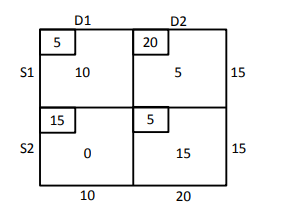
\includegraphics[width=0.75\columnwidth]{chapters/10/7/2/4/figs/fig.png}
 \end{center}
\caption{}
\label{fig:10/7/2/4Fig1}
\end{figure}
\fi

\item Find the position vector of the mid point of the vector joining the points $\vec{P}$(2, 3, 4)
and $\vec{Q}$(4, 1, –2).
\\
\solution
		\begin{enumerate}[label=\thesubsection.\arabic*,ref=\thesubsection.\theenumi]
\item Find the coordinates of the point which divides the join of $(-1,7) $ and $ (4,-3)$ in the ratio 2:3.
	\\
		\solution
	\input{chapters/10/7/2/1/section.tex}
\item Find the coordinates of the point $\vec{R}$ on the line segment joining the points $\vec{P}(-1,3)$ and $\vec{Q}(2,5)$ such that $PR=\frac{3}{5}PQ$.
\item Find the ratio in which the point $\vec{P}\brak{\frac{3}{4},\frac{5}{12}}$ divides the line segment joining the points $\vec{A}\brak{\frac{1}{2},\frac{3}{2}}$ and $ \vec{B}(2,-5)$.
\item Find the coordinates of the point which divides the line segment joining the points $(4,-3)$ and $(8,5)$ in the ratio $3:1$ internally.
\item Find the coordinates of the point $\vec{P}$ on $AD$ such that $AP : PD = 2 : 1$.
\item If the point $\vec{P} (2, 1)$ lies on the line segment joining points $\vec{A} (4, 2)$  and $ \vec{B} (8, 4)$,
then
\begin{enumerate}
	\item $AP =\frac{1}{3}{AB}$ 
\item ${AP}={PE}$
\item ${PB}=\frac{1}{3}{AB}$
\item${AP}=\frac{1}{2}{AB}$
 \end{enumerate}
\item Find the ratio in which the line segment joining the points $(-3,10)$  and  $(6,-8)$  is divided by $ (-1,6)$.
	\\
		\solution
	\input{chapters/10/7/2/4/section.tex}
\item Find the position vector of the mid point of the vector joining the points $\vec{P}$(2, 3, 4)
and $\vec{Q}$(4, 1, –2).
\\
\solution
		\input{chapters/12/10/2/16/section.tex}
\item Let $\vec{A}(4, 2), \vec{B}(6, 5)$  and $ \vec{C}(1, 4)$ be the vertices of $\triangle ABC$.
\begin{enumerate}
\item If $\vec{A}$ and  $\vec{B}$ are $(-2,-2)$ and  $(2,-4)$, respectively, find the coordinates of $\vec{P}$ such that $AP= \frac {3}{7}AB$  and $ \vec{P}$ lies on the line segment $AB$.
	\\
		\solution
	\input{chapters/10/7/2/8/section.tex}
\item Find the coordinates of the points which divide the line segment joining $A(-2,2)$  and  $\vec{B}(2,8)$ into four equal parts.
	\\
		\solution
	\input{chapters/10/7/2/9/section.tex}
\item In what ratio does the point $(-4,6)$ divide the line segment joining the points $\vec{A}(-6,0)$ and $\vec{B}(3,-8)$?
\item Given that $\vec{P}(3,2,-4), \vec{Q}(5,4,-6)$ and $\vec{R}(9,8,-10)$ are collinear. Find the ratio in which $\vec{Q}$ divides $PR$.
\item Points $\vec{A}(-6,10),\vec{B}(-4,6)$  and  $\vec{C}(3,-8)$ are collinear such that $AB=  \frac{2}{9}AC$.
\item The point which divides the line segment joining the points $\vec{P} (7, –6) $  and  $\vec{Q}(3, 4)$ in the 
ratio 1 : 2 internally lies in  which quadrant?
\item Find the coordinates of the points of trisection of the line segment joining $(4,-1)$  and  $(-2,3)$.
	\\
		\solution
	\input{chapters/10/7/2/2/section.tex}
\item Find the coordinates of the points which trisect the line segment joining the points $\vec{P}(4,2,-6)$ and $\vec{Q}(10,-16,6)$.
\item Find the coordinates of the points of trisection (i.e. points dividing to three equal parts) of the line segment joining the points $\vec{A}(2,-2)$ and $\vec{B}(-7,4)$.
\item Point $\vec{P}(5,-3)$ is one of the two points of trisection of line segment joining the points $\vec{A}(7,-2)$ and $\vec{B}(1,-5)$
\item Find the position vector of a point $\vec{R}$ which divides the line joining two points $\vec{P}$
and $\vec{Q}$ whose position vectors are $\hat{i}+2\hat{j}-\hat{k}$ and $-\hat{i}+\hat{j}+\hat{k}$ respectively, in the
ratio 2 : 1
\begin{enumerate}
    \item  internally
    \item  externally
\end{enumerate}
%\solution
%		\input{chapters/12/10/2/15/section.tex}
\item Find the coordinates of the point which divides the line segment joining the points which divides the line segment joining  the points $(-2,3,5)$ and $(1,-4,6)$ in the ratio 
\begin{enumerate}
\item $2:3$ internally,
\item $2:3$ externally
\end{enumerate}
\item Find the coordinates of the point which divides the line segment joining the points $(1,-2,3)$ and $(3,4,-5)$ in the ratio $2:3$
\begin{enumerate}
\item internally, and
\item externally
\end{enumerate}
\item Consider two points $\vec{P}$ and $\vec{Q}$ with position vectors $\overrightarrow{OP} = 3\overrightarrow{a}-2\overrightarrow{b}$ and $\overrightarrow{OQ}=\overrightarrow{a}+\overrightarrow{b}$. Find the position vector of a point $\vec{R}$ which divides the line joining $\vec{P}$ and $\vec{Q}$ in the ratio $2:1$, 
\begin{enumerate}
\item internally, and 
\item externally.
\end{enumerate}
\item The median from $\vec{A}$ meets $BC$ at $\vec{D}$. Find the coordinates of the point $\vec{D}$.
\item Find the coordinates of points $\vec{Q}$ and $\vec{R}$ on medians $BE$ and $CF$ respectively such that $BQ : QE = 2 : 1$  and  $CR : RF = 2 : 1$.
\item What do you observe?
\item If $\vec{A}, \vec{B}$ and $\vec{C}$  are the vertices of $\triangle ABC$, find the coordinates of the centroid of the triangle.
\end{enumerate}
\solution
	\input{chapters/10/7/4/7/section.tex}
\item If $\vec{P}(9a-2,-b)$ divides line segment joining $\vec{A}(3a+1,-3)$ and $\vec{B}(8a,5)$ in the ratio 3:1, find the values of $a$ and $b$.
\item Find the position vector of a point $\vec{R}$ which divides the line joining two points $\vec{P}$ and $\vec{Q}$ whose position vectors are $2\vec{a}+\vec{b}$ and $\vec{a}-3\vec{b}$ externally in the ratio $1:2$.
\item The position vector of the point which divides the join of points 2$\vec{a}$-3$\vec{b}$ $\text{and}$ $\vec{a}+\vec{b}$ in the ratio 3:1 is \rule{1cm}{0.1pt}.
\item If $\vec{a}$ and $\vec{b}$ are the postion vectors of $\vec{A}$ and $\vec{B}$, respectively, find the position vector of a point $\vec{C}$ in $BA$ produced such that $BC=1.5BA$.
\item Find the position vector of a point $\vec{R}$ which divides the line joining two points $\vec{P}$ and $\vec{Q}$ whose position vectors are $(2\vec{a}+\vec{b})$ and $(\vec{a}-3\vec{b})$
externally in the ratio 1 : 2. Also, show that $\vec{P}$ is the mid point of the line segment $RQ$.
\end{enumerate}

\item Let $\vec{A}(4, 2), \vec{B}(6, 5)$  and $ \vec{C}(1, 4)$ be the vertices of $\triangle ABC$.
\begin{enumerate}
\item If $\vec{A}$ and  $\vec{B}$ are $(-2,-2)$ and  $(2,-4)$, respectively, find the coordinates of $\vec{P}$ such that $AP= \frac {3}{7}AB$  and $ \vec{P}$ lies on the line segment $AB$.
	\\
		\solution
	\begin{enumerate}[label=\thesubsection.\arabic*,ref=\thesubsection.\theenumi]
\item Find the coordinates of the point which divides the join of $(-1,7) $ and $ (4,-3)$ in the ratio 2:3.
	\\
		\solution
	\input{chapters/10/7/2/1/section.tex}
\item Find the coordinates of the point $\vec{R}$ on the line segment joining the points $\vec{P}(-1,3)$ and $\vec{Q}(2,5)$ such that $PR=\frac{3}{5}PQ$.
\item Find the ratio in which the point $\vec{P}\brak{\frac{3}{4},\frac{5}{12}}$ divides the line segment joining the points $\vec{A}\brak{\frac{1}{2},\frac{3}{2}}$ and $ \vec{B}(2,-5)$.
\item Find the coordinates of the point which divides the line segment joining the points $(4,-3)$ and $(8,5)$ in the ratio $3:1$ internally.
\item Find the coordinates of the point $\vec{P}$ on $AD$ such that $AP : PD = 2 : 1$.
\item If the point $\vec{P} (2, 1)$ lies on the line segment joining points $\vec{A} (4, 2)$  and $ \vec{B} (8, 4)$,
then
\begin{enumerate}
	\item $AP =\frac{1}{3}{AB}$ 
\item ${AP}={PE}$
\item ${PB}=\frac{1}{3}{AB}$
\item${AP}=\frac{1}{2}{AB}$
 \end{enumerate}
\item Find the ratio in which the line segment joining the points $(-3,10)$  and  $(6,-8)$  is divided by $ (-1,6)$.
	\\
		\solution
	\input{chapters/10/7/2/4/section.tex}
\item Find the position vector of the mid point of the vector joining the points $\vec{P}$(2, 3, 4)
and $\vec{Q}$(4, 1, –2).
\\
\solution
		\input{chapters/12/10/2/16/section.tex}
\item Let $\vec{A}(4, 2), \vec{B}(6, 5)$  and $ \vec{C}(1, 4)$ be the vertices of $\triangle ABC$.
\begin{enumerate}
\item If $\vec{A}$ and  $\vec{B}$ are $(-2,-2)$ and  $(2,-4)$, respectively, find the coordinates of $\vec{P}$ such that $AP= \frac {3}{7}AB$  and $ \vec{P}$ lies on the line segment $AB$.
	\\
		\solution
	\input{chapters/10/7/2/8/section.tex}
\item Find the coordinates of the points which divide the line segment joining $A(-2,2)$  and  $\vec{B}(2,8)$ into four equal parts.
	\\
		\solution
	\input{chapters/10/7/2/9/section.tex}
\item In what ratio does the point $(-4,6)$ divide the line segment joining the points $\vec{A}(-6,0)$ and $\vec{B}(3,-8)$?
\item Given that $\vec{P}(3,2,-4), \vec{Q}(5,4,-6)$ and $\vec{R}(9,8,-10)$ are collinear. Find the ratio in which $\vec{Q}$ divides $PR$.
\item Points $\vec{A}(-6,10),\vec{B}(-4,6)$  and  $\vec{C}(3,-8)$ are collinear such that $AB=  \frac{2}{9}AC$.
\item The point which divides the line segment joining the points $\vec{P} (7, –6) $  and  $\vec{Q}(3, 4)$ in the 
ratio 1 : 2 internally lies in  which quadrant?
\item Find the coordinates of the points of trisection of the line segment joining $(4,-1)$  and  $(-2,3)$.
	\\
		\solution
	\input{chapters/10/7/2/2/section.tex}
\item Find the coordinates of the points which trisect the line segment joining the points $\vec{P}(4,2,-6)$ and $\vec{Q}(10,-16,6)$.
\item Find the coordinates of the points of trisection (i.e. points dividing to three equal parts) of the line segment joining the points $\vec{A}(2,-2)$ and $\vec{B}(-7,4)$.
\item Point $\vec{P}(5,-3)$ is one of the two points of trisection of line segment joining the points $\vec{A}(7,-2)$ and $\vec{B}(1,-5)$
\item Find the position vector of a point $\vec{R}$ which divides the line joining two points $\vec{P}$
and $\vec{Q}$ whose position vectors are $\hat{i}+2\hat{j}-\hat{k}$ and $-\hat{i}+\hat{j}+\hat{k}$ respectively, in the
ratio 2 : 1
\begin{enumerate}
    \item  internally
    \item  externally
\end{enumerate}
%\solution
%		\input{chapters/12/10/2/15/section.tex}
\item Find the coordinates of the point which divides the line segment joining the points which divides the line segment joining  the points $(-2,3,5)$ and $(1,-4,6)$ in the ratio 
\begin{enumerate}
\item $2:3$ internally,
\item $2:3$ externally
\end{enumerate}
\item Find the coordinates of the point which divides the line segment joining the points $(1,-2,3)$ and $(3,4,-5)$ in the ratio $2:3$
\begin{enumerate}
\item internally, and
\item externally
\end{enumerate}
\item Consider two points $\vec{P}$ and $\vec{Q}$ with position vectors $\overrightarrow{OP} = 3\overrightarrow{a}-2\overrightarrow{b}$ and $\overrightarrow{OQ}=\overrightarrow{a}+\overrightarrow{b}$. Find the position vector of a point $\vec{R}$ which divides the line joining $\vec{P}$ and $\vec{Q}$ in the ratio $2:1$, 
\begin{enumerate}
\item internally, and 
\item externally.
\end{enumerate}
\item The median from $\vec{A}$ meets $BC$ at $\vec{D}$. Find the coordinates of the point $\vec{D}$.
\item Find the coordinates of points $\vec{Q}$ and $\vec{R}$ on medians $BE$ and $CF$ respectively such that $BQ : QE = 2 : 1$  and  $CR : RF = 2 : 1$.
\item What do you observe?
\item If $\vec{A}, \vec{B}$ and $\vec{C}$  are the vertices of $\triangle ABC$, find the coordinates of the centroid of the triangle.
\end{enumerate}
\solution
	\input{chapters/10/7/4/7/section.tex}
\item If $\vec{P}(9a-2,-b)$ divides line segment joining $\vec{A}(3a+1,-3)$ and $\vec{B}(8a,5)$ in the ratio 3:1, find the values of $a$ and $b$.
\item Find the position vector of a point $\vec{R}$ which divides the line joining two points $\vec{P}$ and $\vec{Q}$ whose position vectors are $2\vec{a}+\vec{b}$ and $\vec{a}-3\vec{b}$ externally in the ratio $1:2$.
\item The position vector of the point which divides the join of points 2$\vec{a}$-3$\vec{b}$ $\text{and}$ $\vec{a}+\vec{b}$ in the ratio 3:1 is \rule{1cm}{0.1pt}.
\item If $\vec{a}$ and $\vec{b}$ are the postion vectors of $\vec{A}$ and $\vec{B}$, respectively, find the position vector of a point $\vec{C}$ in $BA$ produced such that $BC=1.5BA$.
\item Find the position vector of a point $\vec{R}$ which divides the line joining two points $\vec{P}$ and $\vec{Q}$ whose position vectors are $(2\vec{a}+\vec{b})$ and $(\vec{a}-3\vec{b})$
externally in the ratio 1 : 2. Also, show that $\vec{P}$ is the mid point of the line segment $RQ$.
\end{enumerate}

\item Find the coordinates of the points which divide the line segment joining $A(-2,2)$  and  $\vec{B}(2,8)$ into four equal parts.
	\\
		\solution
	\begin{enumerate}[label=\thesubsection.\arabic*,ref=\thesubsection.\theenumi]
\item Find the coordinates of the point which divides the join of $(-1,7) $ and $ (4,-3)$ in the ratio 2:3.
	\\
		\solution
	\input{chapters/10/7/2/1/section.tex}
\item Find the coordinates of the point $\vec{R}$ on the line segment joining the points $\vec{P}(-1,3)$ and $\vec{Q}(2,5)$ such that $PR=\frac{3}{5}PQ$.
\item Find the ratio in which the point $\vec{P}\brak{\frac{3}{4},\frac{5}{12}}$ divides the line segment joining the points $\vec{A}\brak{\frac{1}{2},\frac{3}{2}}$ and $ \vec{B}(2,-5)$.
\item Find the coordinates of the point which divides the line segment joining the points $(4,-3)$ and $(8,5)$ in the ratio $3:1$ internally.
\item Find the coordinates of the point $\vec{P}$ on $AD$ such that $AP : PD = 2 : 1$.
\item If the point $\vec{P} (2, 1)$ lies on the line segment joining points $\vec{A} (4, 2)$  and $ \vec{B} (8, 4)$,
then
\begin{enumerate}
	\item $AP =\frac{1}{3}{AB}$ 
\item ${AP}={PE}$
\item ${PB}=\frac{1}{3}{AB}$
\item${AP}=\frac{1}{2}{AB}$
 \end{enumerate}
\item Find the ratio in which the line segment joining the points $(-3,10)$  and  $(6,-8)$  is divided by $ (-1,6)$.
	\\
		\solution
	\input{chapters/10/7/2/4/section.tex}
\item Find the position vector of the mid point of the vector joining the points $\vec{P}$(2, 3, 4)
and $\vec{Q}$(4, 1, –2).
\\
\solution
		\input{chapters/12/10/2/16/section.tex}
\item Let $\vec{A}(4, 2), \vec{B}(6, 5)$  and $ \vec{C}(1, 4)$ be the vertices of $\triangle ABC$.
\begin{enumerate}
\item If $\vec{A}$ and  $\vec{B}$ are $(-2,-2)$ and  $(2,-4)$, respectively, find the coordinates of $\vec{P}$ such that $AP= \frac {3}{7}AB$  and $ \vec{P}$ lies on the line segment $AB$.
	\\
		\solution
	\input{chapters/10/7/2/8/section.tex}
\item Find the coordinates of the points which divide the line segment joining $A(-2,2)$  and  $\vec{B}(2,8)$ into four equal parts.
	\\
		\solution
	\input{chapters/10/7/2/9/section.tex}
\item In what ratio does the point $(-4,6)$ divide the line segment joining the points $\vec{A}(-6,0)$ and $\vec{B}(3,-8)$?
\item Given that $\vec{P}(3,2,-4), \vec{Q}(5,4,-6)$ and $\vec{R}(9,8,-10)$ are collinear. Find the ratio in which $\vec{Q}$ divides $PR$.
\item Points $\vec{A}(-6,10),\vec{B}(-4,6)$  and  $\vec{C}(3,-8)$ are collinear such that $AB=  \frac{2}{9}AC$.
\item The point which divides the line segment joining the points $\vec{P} (7, –6) $  and  $\vec{Q}(3, 4)$ in the 
ratio 1 : 2 internally lies in  which quadrant?
\item Find the coordinates of the points of trisection of the line segment joining $(4,-1)$  and  $(-2,3)$.
	\\
		\solution
	\input{chapters/10/7/2/2/section.tex}
\item Find the coordinates of the points which trisect the line segment joining the points $\vec{P}(4,2,-6)$ and $\vec{Q}(10,-16,6)$.
\item Find the coordinates of the points of trisection (i.e. points dividing to three equal parts) of the line segment joining the points $\vec{A}(2,-2)$ and $\vec{B}(-7,4)$.
\item Point $\vec{P}(5,-3)$ is one of the two points of trisection of line segment joining the points $\vec{A}(7,-2)$ and $\vec{B}(1,-5)$
\item Find the position vector of a point $\vec{R}$ which divides the line joining two points $\vec{P}$
and $\vec{Q}$ whose position vectors are $\hat{i}+2\hat{j}-\hat{k}$ and $-\hat{i}+\hat{j}+\hat{k}$ respectively, in the
ratio 2 : 1
\begin{enumerate}
    \item  internally
    \item  externally
\end{enumerate}
%\solution
%		\input{chapters/12/10/2/15/section.tex}
\item Find the coordinates of the point which divides the line segment joining the points which divides the line segment joining  the points $(-2,3,5)$ and $(1,-4,6)$ in the ratio 
\begin{enumerate}
\item $2:3$ internally,
\item $2:3$ externally
\end{enumerate}
\item Find the coordinates of the point which divides the line segment joining the points $(1,-2,3)$ and $(3,4,-5)$ in the ratio $2:3$
\begin{enumerate}
\item internally, and
\item externally
\end{enumerate}
\item Consider two points $\vec{P}$ and $\vec{Q}$ with position vectors $\overrightarrow{OP} = 3\overrightarrow{a}-2\overrightarrow{b}$ and $\overrightarrow{OQ}=\overrightarrow{a}+\overrightarrow{b}$. Find the position vector of a point $\vec{R}$ which divides the line joining $\vec{P}$ and $\vec{Q}$ in the ratio $2:1$, 
\begin{enumerate}
\item internally, and 
\item externally.
\end{enumerate}
\item The median from $\vec{A}$ meets $BC$ at $\vec{D}$. Find the coordinates of the point $\vec{D}$.
\item Find the coordinates of points $\vec{Q}$ and $\vec{R}$ on medians $BE$ and $CF$ respectively such that $BQ : QE = 2 : 1$  and  $CR : RF = 2 : 1$.
\item What do you observe?
\item If $\vec{A}, \vec{B}$ and $\vec{C}$  are the vertices of $\triangle ABC$, find the coordinates of the centroid of the triangle.
\end{enumerate}
\solution
	\input{chapters/10/7/4/7/section.tex}
\item If $\vec{P}(9a-2,-b)$ divides line segment joining $\vec{A}(3a+1,-3)$ and $\vec{B}(8a,5)$ in the ratio 3:1, find the values of $a$ and $b$.
\item Find the position vector of a point $\vec{R}$ which divides the line joining two points $\vec{P}$ and $\vec{Q}$ whose position vectors are $2\vec{a}+\vec{b}$ and $\vec{a}-3\vec{b}$ externally in the ratio $1:2$.
\item The position vector of the point which divides the join of points 2$\vec{a}$-3$\vec{b}$ $\text{and}$ $\vec{a}+\vec{b}$ in the ratio 3:1 is \rule{1cm}{0.1pt}.
\item If $\vec{a}$ and $\vec{b}$ are the postion vectors of $\vec{A}$ and $\vec{B}$, respectively, find the position vector of a point $\vec{C}$ in $BA$ produced such that $BC=1.5BA$.
\item Find the position vector of a point $\vec{R}$ which divides the line joining two points $\vec{P}$ and $\vec{Q}$ whose position vectors are $(2\vec{a}+\vec{b})$ and $(\vec{a}-3\vec{b})$
externally in the ratio 1 : 2. Also, show that $\vec{P}$ is the mid point of the line segment $RQ$.
\end{enumerate}

\item In what ratio does the point $(-4,6)$ divide the line segment joining the points $\vec{A}(-6,0)$ and $\vec{B}(3,-8)$?
\item Given that $\vec{P}(3,2,-4), \vec{Q}(5,4,-6)$ and $\vec{R}(9,8,-10)$ are collinear. Find the ratio in which $\vec{Q}$ divides $PR$.
\item Points $\vec{A}(-6,10),\vec{B}(-4,6)$  and  $\vec{C}(3,-8)$ are collinear such that $AB=  \frac{2}{9}AC$.
\item The point which divides the line segment joining the points $\vec{P} (7, –6) $  and  $\vec{Q}(3, 4)$ in the 
ratio 1 : 2 internally lies in  which quadrant?
\item Find the coordinates of the points of trisection of the line segment joining $(4,-1)$  and  $(-2,3)$.
	\\
		\solution
	Using section formula,
\begin{align}
\vec{R}=\frac{1}{1+\frac{1}{2}}\brak{\myvec{4\\-1}+\frac{1}{2}\myvec{-2\\3}}
=\myvec{2\\ \frac{1}{3}}\\
\vec{S}=\frac{1}{1+\frac{2}{1}}\brak{\myvec{4\\-1}+\frac{2}{1}\myvec{-2\\3}}
=\myvec{0\\ \frac{5}{3}}
\end{align}
which are the desired points of trisection.
\iffalse
See
		\figref{fig:chapters/10/7/2/2/Figure}
\begin{figure}[H]
\centering
\includegraphics[width=0.75\columnwidth]{chapters/10/7/2/2/figs/dj.pdf}
\caption{}
		\label{fig:chapters/10/7/2/2/Figure}
\end{figure}
\fi

\item Find the coordinates of the points which trisect the line segment joining the points $\vec{P}(4,2,-6)$ and $\vec{Q}(10,-16,6)$.
\item Find the coordinates of the points of trisection (i.e. points dividing to three equal parts) of the line segment joining the points $\vec{A}(2,-2)$ and $\vec{B}(-7,4)$.
\item Point $\vec{P}(5,-3)$ is one of the two points of trisection of line segment joining the points $\vec{A}(7,-2)$ and $\vec{B}(1,-5)$
\item Find the position vector of a point $\vec{R}$ which divides the line joining two points $\vec{P}$
and $\vec{Q}$ whose position vectors are $\hat{i}+2\hat{j}-\hat{k}$ and $-\hat{i}+\hat{j}+\hat{k}$ respectively, in the
ratio 2 : 1
\begin{enumerate}
    \item  internally
    \item  externally
\end{enumerate}
%\solution
%		\begin{enumerate}[label=\thesubsection.\arabic*,ref=\thesubsection.\theenumi]
\item Find the coordinates of the point which divides the join of $(-1,7) $ and $ (4,-3)$ in the ratio 2:3.
	\\
		\solution
	\input{chapters/10/7/2/1/section.tex}
\item Find the coordinates of the point $\vec{R}$ on the line segment joining the points $\vec{P}(-1,3)$ and $\vec{Q}(2,5)$ such that $PR=\frac{3}{5}PQ$.
\item Find the ratio in which the point $\vec{P}\brak{\frac{3}{4},\frac{5}{12}}$ divides the line segment joining the points $\vec{A}\brak{\frac{1}{2},\frac{3}{2}}$ and $ \vec{B}(2,-5)$.
\item Find the coordinates of the point which divides the line segment joining the points $(4,-3)$ and $(8,5)$ in the ratio $3:1$ internally.
\item Find the coordinates of the point $\vec{P}$ on $AD$ such that $AP : PD = 2 : 1$.
\item If the point $\vec{P} (2, 1)$ lies on the line segment joining points $\vec{A} (4, 2)$  and $ \vec{B} (8, 4)$,
then
\begin{enumerate}
	\item $AP =\frac{1}{3}{AB}$ 
\item ${AP}={PE}$
\item ${PB}=\frac{1}{3}{AB}$
\item${AP}=\frac{1}{2}{AB}$
 \end{enumerate}
\item Find the ratio in which the line segment joining the points $(-3,10)$  and  $(6,-8)$  is divided by $ (-1,6)$.
	\\
		\solution
	\input{chapters/10/7/2/4/section.tex}
\item Find the position vector of the mid point of the vector joining the points $\vec{P}$(2, 3, 4)
and $\vec{Q}$(4, 1, –2).
\\
\solution
		\input{chapters/12/10/2/16/section.tex}
\item Let $\vec{A}(4, 2), \vec{B}(6, 5)$  and $ \vec{C}(1, 4)$ be the vertices of $\triangle ABC$.
\begin{enumerate}
\item If $\vec{A}$ and  $\vec{B}$ are $(-2,-2)$ and  $(2,-4)$, respectively, find the coordinates of $\vec{P}$ such that $AP= \frac {3}{7}AB$  and $ \vec{P}$ lies on the line segment $AB$.
	\\
		\solution
	\input{chapters/10/7/2/8/section.tex}
\item Find the coordinates of the points which divide the line segment joining $A(-2,2)$  and  $\vec{B}(2,8)$ into four equal parts.
	\\
		\solution
	\input{chapters/10/7/2/9/section.tex}
\item In what ratio does the point $(-4,6)$ divide the line segment joining the points $\vec{A}(-6,0)$ and $\vec{B}(3,-8)$?
\item Given that $\vec{P}(3,2,-4), \vec{Q}(5,4,-6)$ and $\vec{R}(9,8,-10)$ are collinear. Find the ratio in which $\vec{Q}$ divides $PR$.
\item Points $\vec{A}(-6,10),\vec{B}(-4,6)$  and  $\vec{C}(3,-8)$ are collinear such that $AB=  \frac{2}{9}AC$.
\item The point which divides the line segment joining the points $\vec{P} (7, –6) $  and  $\vec{Q}(3, 4)$ in the 
ratio 1 : 2 internally lies in  which quadrant?
\item Find the coordinates of the points of trisection of the line segment joining $(4,-1)$  and  $(-2,3)$.
	\\
		\solution
	\input{chapters/10/7/2/2/section.tex}
\item Find the coordinates of the points which trisect the line segment joining the points $\vec{P}(4,2,-6)$ and $\vec{Q}(10,-16,6)$.
\item Find the coordinates of the points of trisection (i.e. points dividing to three equal parts) of the line segment joining the points $\vec{A}(2,-2)$ and $\vec{B}(-7,4)$.
\item Point $\vec{P}(5,-3)$ is one of the two points of trisection of line segment joining the points $\vec{A}(7,-2)$ and $\vec{B}(1,-5)$
\item Find the position vector of a point $\vec{R}$ which divides the line joining two points $\vec{P}$
and $\vec{Q}$ whose position vectors are $\hat{i}+2\hat{j}-\hat{k}$ and $-\hat{i}+\hat{j}+\hat{k}$ respectively, in the
ratio 2 : 1
\begin{enumerate}
    \item  internally
    \item  externally
\end{enumerate}
%\solution
%		\input{chapters/12/10/2/15/section.tex}
\item Find the coordinates of the point which divides the line segment joining the points which divides the line segment joining  the points $(-2,3,5)$ and $(1,-4,6)$ in the ratio 
\begin{enumerate}
\item $2:3$ internally,
\item $2:3$ externally
\end{enumerate}
\item Find the coordinates of the point which divides the line segment joining the points $(1,-2,3)$ and $(3,4,-5)$ in the ratio $2:3$
\begin{enumerate}
\item internally, and
\item externally
\end{enumerate}
\item Consider two points $\vec{P}$ and $\vec{Q}$ with position vectors $\overrightarrow{OP} = 3\overrightarrow{a}-2\overrightarrow{b}$ and $\overrightarrow{OQ}=\overrightarrow{a}+\overrightarrow{b}$. Find the position vector of a point $\vec{R}$ which divides the line joining $\vec{P}$ and $\vec{Q}$ in the ratio $2:1$, 
\begin{enumerate}
\item internally, and 
\item externally.
\end{enumerate}
\item The median from $\vec{A}$ meets $BC$ at $\vec{D}$. Find the coordinates of the point $\vec{D}$.
\item Find the coordinates of points $\vec{Q}$ and $\vec{R}$ on medians $BE$ and $CF$ respectively such that $BQ : QE = 2 : 1$  and  $CR : RF = 2 : 1$.
\item What do you observe?
\item If $\vec{A}, \vec{B}$ and $\vec{C}$  are the vertices of $\triangle ABC$, find the coordinates of the centroid of the triangle.
\end{enumerate}
\solution
	\input{chapters/10/7/4/7/section.tex}
\item If $\vec{P}(9a-2,-b)$ divides line segment joining $\vec{A}(3a+1,-3)$ and $\vec{B}(8a,5)$ in the ratio 3:1, find the values of $a$ and $b$.
\item Find the position vector of a point $\vec{R}$ which divides the line joining two points $\vec{P}$ and $\vec{Q}$ whose position vectors are $2\vec{a}+\vec{b}$ and $\vec{a}-3\vec{b}$ externally in the ratio $1:2$.
\item The position vector of the point which divides the join of points 2$\vec{a}$-3$\vec{b}$ $\text{and}$ $\vec{a}+\vec{b}$ in the ratio 3:1 is \rule{1cm}{0.1pt}.
\item If $\vec{a}$ and $\vec{b}$ are the postion vectors of $\vec{A}$ and $\vec{B}$, respectively, find the position vector of a point $\vec{C}$ in $BA$ produced such that $BC=1.5BA$.
\item Find the position vector of a point $\vec{R}$ which divides the line joining two points $\vec{P}$ and $\vec{Q}$ whose position vectors are $(2\vec{a}+\vec{b})$ and $(\vec{a}-3\vec{b})$
externally in the ratio 1 : 2. Also, show that $\vec{P}$ is the mid point of the line segment $RQ$.
\end{enumerate}

\item Find the coordinates of the point which divides the line segment joining the points which divides the line segment joining  the points $(-2,3,5)$ and $(1,-4,6)$ in the ratio 
\begin{enumerate}
\item $2:3$ internally,
\item $2:3$ externally
\end{enumerate}
\item Find the coordinates of the point which divides the line segment joining the points $(1,-2,3)$ and $(3,4,-5)$ in the ratio $2:3$
\begin{enumerate}
\item internally, and
\item externally
\end{enumerate}
\item Consider two points $\vec{P}$ and $\vec{Q}$ with position vectors $\overrightarrow{OP} = 3\overrightarrow{a}-2\overrightarrow{b}$ and $\overrightarrow{OQ}=\overrightarrow{a}+\overrightarrow{b}$. Find the position vector of a point $\vec{R}$ which divides the line joining $\vec{P}$ and $\vec{Q}$ in the ratio $2:1$, 
\begin{enumerate}
\item internally, and 
\item externally.
\end{enumerate}
\item The median from $\vec{A}$ meets $BC$ at $\vec{D}$. Find the coordinates of the point $\vec{D}$.
\item Find the coordinates of points $\vec{Q}$ and $\vec{R}$ on medians $BE$ and $CF$ respectively such that $BQ : QE = 2 : 1$  and  $CR : RF = 2 : 1$.
\item What do you observe?
\item If $\vec{A}, \vec{B}$ and $\vec{C}$  are the vertices of $\triangle ABC$, find the coordinates of the centroid of the triangle.
\end{enumerate}
\solution
	\begin{enumerate}[label=\thesubsection.\arabic*,ref=\thesubsection.\theenumi]
\item Find the coordinates of the point which divides the join of $(-1,7) $ and $ (4,-3)$ in the ratio 2:3.
	\\
		\solution
	\input{chapters/10/7/2/1/section.tex}
\item Find the coordinates of the point $\vec{R}$ on the line segment joining the points $\vec{P}(-1,3)$ and $\vec{Q}(2,5)$ such that $PR=\frac{3}{5}PQ$.
\item Find the ratio in which the point $\vec{P}\brak{\frac{3}{4},\frac{5}{12}}$ divides the line segment joining the points $\vec{A}\brak{\frac{1}{2},\frac{3}{2}}$ and $ \vec{B}(2,-5)$.
\item Find the coordinates of the point which divides the line segment joining the points $(4,-3)$ and $(8,5)$ in the ratio $3:1$ internally.
\item Find the coordinates of the point $\vec{P}$ on $AD$ such that $AP : PD = 2 : 1$.
\item If the point $\vec{P} (2, 1)$ lies on the line segment joining points $\vec{A} (4, 2)$  and $ \vec{B} (8, 4)$,
then
\begin{enumerate}
	\item $AP =\frac{1}{3}{AB}$ 
\item ${AP}={PE}$
\item ${PB}=\frac{1}{3}{AB}$
\item${AP}=\frac{1}{2}{AB}$
 \end{enumerate}
\item Find the ratio in which the line segment joining the points $(-3,10)$  and  $(6,-8)$  is divided by $ (-1,6)$.
	\\
		\solution
	\input{chapters/10/7/2/4/section.tex}
\item Find the position vector of the mid point of the vector joining the points $\vec{P}$(2, 3, 4)
and $\vec{Q}$(4, 1, –2).
\\
\solution
		\input{chapters/12/10/2/16/section.tex}
\item Let $\vec{A}(4, 2), \vec{B}(6, 5)$  and $ \vec{C}(1, 4)$ be the vertices of $\triangle ABC$.
\begin{enumerate}
\item If $\vec{A}$ and  $\vec{B}$ are $(-2,-2)$ and  $(2,-4)$, respectively, find the coordinates of $\vec{P}$ such that $AP= \frac {3}{7}AB$  and $ \vec{P}$ lies on the line segment $AB$.
	\\
		\solution
	\input{chapters/10/7/2/8/section.tex}
\item Find the coordinates of the points which divide the line segment joining $A(-2,2)$  and  $\vec{B}(2,8)$ into four equal parts.
	\\
		\solution
	\input{chapters/10/7/2/9/section.tex}
\item In what ratio does the point $(-4,6)$ divide the line segment joining the points $\vec{A}(-6,0)$ and $\vec{B}(3,-8)$?
\item Given that $\vec{P}(3,2,-4), \vec{Q}(5,4,-6)$ and $\vec{R}(9,8,-10)$ are collinear. Find the ratio in which $\vec{Q}$ divides $PR$.
\item Points $\vec{A}(-6,10),\vec{B}(-4,6)$  and  $\vec{C}(3,-8)$ are collinear such that $AB=  \frac{2}{9}AC$.
\item The point which divides the line segment joining the points $\vec{P} (7, –6) $  and  $\vec{Q}(3, 4)$ in the 
ratio 1 : 2 internally lies in  which quadrant?
\item Find the coordinates of the points of trisection of the line segment joining $(4,-1)$  and  $(-2,3)$.
	\\
		\solution
	\input{chapters/10/7/2/2/section.tex}
\item Find the coordinates of the points which trisect the line segment joining the points $\vec{P}(4,2,-6)$ and $\vec{Q}(10,-16,6)$.
\item Find the coordinates of the points of trisection (i.e. points dividing to three equal parts) of the line segment joining the points $\vec{A}(2,-2)$ and $\vec{B}(-7,4)$.
\item Point $\vec{P}(5,-3)$ is one of the two points of trisection of line segment joining the points $\vec{A}(7,-2)$ and $\vec{B}(1,-5)$
\item Find the position vector of a point $\vec{R}$ which divides the line joining two points $\vec{P}$
and $\vec{Q}$ whose position vectors are $\hat{i}+2\hat{j}-\hat{k}$ and $-\hat{i}+\hat{j}+\hat{k}$ respectively, in the
ratio 2 : 1
\begin{enumerate}
    \item  internally
    \item  externally
\end{enumerate}
%\solution
%		\input{chapters/12/10/2/15/section.tex}
\item Find the coordinates of the point which divides the line segment joining the points which divides the line segment joining  the points $(-2,3,5)$ and $(1,-4,6)$ in the ratio 
\begin{enumerate}
\item $2:3$ internally,
\item $2:3$ externally
\end{enumerate}
\item Find the coordinates of the point which divides the line segment joining the points $(1,-2,3)$ and $(3,4,-5)$ in the ratio $2:3$
\begin{enumerate}
\item internally, and
\item externally
\end{enumerate}
\item Consider two points $\vec{P}$ and $\vec{Q}$ with position vectors $\overrightarrow{OP} = 3\overrightarrow{a}-2\overrightarrow{b}$ and $\overrightarrow{OQ}=\overrightarrow{a}+\overrightarrow{b}$. Find the position vector of a point $\vec{R}$ which divides the line joining $\vec{P}$ and $\vec{Q}$ in the ratio $2:1$, 
\begin{enumerate}
\item internally, and 
\item externally.
\end{enumerate}
\item The median from $\vec{A}$ meets $BC$ at $\vec{D}$. Find the coordinates of the point $\vec{D}$.
\item Find the coordinates of points $\vec{Q}$ and $\vec{R}$ on medians $BE$ and $CF$ respectively such that $BQ : QE = 2 : 1$  and  $CR : RF = 2 : 1$.
\item What do you observe?
\item If $\vec{A}, \vec{B}$ and $\vec{C}$  are the vertices of $\triangle ABC$, find the coordinates of the centroid of the triangle.
\end{enumerate}
\solution
	\input{chapters/10/7/4/7/section.tex}
\item If $\vec{P}(9a-2,-b)$ divides line segment joining $\vec{A}(3a+1,-3)$ and $\vec{B}(8a,5)$ in the ratio 3:1, find the values of $a$ and $b$.
\item Find the position vector of a point $\vec{R}$ which divides the line joining two points $\vec{P}$ and $\vec{Q}$ whose position vectors are $2\vec{a}+\vec{b}$ and $\vec{a}-3\vec{b}$ externally in the ratio $1:2$.
\item The position vector of the point which divides the join of points 2$\vec{a}$-3$\vec{b}$ $\text{and}$ $\vec{a}+\vec{b}$ in the ratio 3:1 is \rule{1cm}{0.1pt}.
\item If $\vec{a}$ and $\vec{b}$ are the postion vectors of $\vec{A}$ and $\vec{B}$, respectively, find the position vector of a point $\vec{C}$ in $BA$ produced such that $BC=1.5BA$.
\item Find the position vector of a point $\vec{R}$ which divides the line joining two points $\vec{P}$ and $\vec{Q}$ whose position vectors are $(2\vec{a}+\vec{b})$ and $(\vec{a}-3\vec{b})$
externally in the ratio 1 : 2. Also, show that $\vec{P}$ is the mid point of the line segment $RQ$.
\end{enumerate}

\item If $\vec{P}(9a-2,-b)$ divides line segment joining $\vec{A}(3a+1,-3)$ and $\vec{B}(8a,5)$ in the ratio 3:1, find the values of $a$ and $b$.
\item Find the position vector of a point $\vec{R}$ which divides the line joining two points $\vec{P}$ and $\vec{Q}$ whose position vectors are $2\vec{a}+\vec{b}$ and $\vec{a}-3\vec{b}$ externally in the ratio $1:2$.
\item The position vector of the point which divides the join of points 2$\vec{a}$-3$\vec{b}$ $\text{and}$ $\vec{a}+\vec{b}$ in the ratio 3:1 is \rule{1cm}{0.1pt}.
\item If $\vec{a}$ and $\vec{b}$ are the postion vectors of $\vec{A}$ and $\vec{B}$, respectively, find the position vector of a point $\vec{C}$ in $BA$ produced such that $BC=1.5BA$.
\item Find the position vector of a point $\vec{R}$ which divides the line joining two points $\vec{P}$ and $\vec{Q}$ whose position vectors are $(2\vec{a}+\vec{b})$ and $(\vec{a}-3\vec{b})$
externally in the ratio 1 : 2. Also, show that $\vec{P}$ is the mid point of the line segment $RQ$.
\end{enumerate}

\item Find the coordinates of the point which divides the line segment joining the points which divides the line segment joining  the points $(-2,3,5)$ and $(1,-4,6)$ in the ratio 
\begin{enumerate}
\item $2:3$ internally,
\item $2:3$ externally
\end{enumerate}
\item Find the coordinates of the point which divides the line segment joining the points $(1,-2,3)$ and $(3,4,-5)$ in the ratio $2:3$
\begin{enumerate}
\item internally, and
\item externally
\end{enumerate}
\item Consider two points $\vec{P}$ and $\vec{Q}$ with position vectors $\overrightarrow{OP} = 3\overrightarrow{a}-2\overrightarrow{b}$ and $\overrightarrow{OQ}=\overrightarrow{a}+\overrightarrow{b}$. Find the position vector of a point $\vec{R}$ which divides the line joining $\vec{P}$ and $\vec{Q}$ in the ratio $2:1$, 
\begin{enumerate}
\item internally, and 
\item externally.
\end{enumerate}
\item The median from $\vec{A}$ meets $BC$ at $\vec{D}$. Find the coordinates of the point $\vec{D}$.
\item Find the coordinates of points $\vec{Q}$ and $\vec{R}$ on medians $BE$ and $CF$ respectively such that $BQ : QE = 2 : 1$  and  $CR : RF = 2 : 1$.
\item What do you observe?
\item If $\vec{A}, \vec{B}$ and $\vec{C}$  are the vertices of $\triangle ABC$, find the coordinates of the centroid of the triangle.
\end{enumerate}
\solution
	\begin{enumerate}[label=\thesubsection.\arabic*,ref=\thesubsection.\theenumi]
\item Find the coordinates of the point which divides the join of $(-1,7) $ and $ (4,-3)$ in the ratio 2:3.
	\\
		\solution
	\begin{enumerate}[label=\thesubsection.\arabic*,ref=\thesubsection.\theenumi]
\item Find the coordinates of the point which divides the join of $(-1,7) $ and $ (4,-3)$ in the ratio 2:3.
	\\
		\solution
	\input{chapters/10/7/2/1/section.tex}
\item Find the coordinates of the point $\vec{R}$ on the line segment joining the points $\vec{P}(-1,3)$ and $\vec{Q}(2,5)$ such that $PR=\frac{3}{5}PQ$.
\item Find the ratio in which the point $\vec{P}\brak{\frac{3}{4},\frac{5}{12}}$ divides the line segment joining the points $\vec{A}\brak{\frac{1}{2},\frac{3}{2}}$ and $ \vec{B}(2,-5)$.
\item Find the coordinates of the point which divides the line segment joining the points $(4,-3)$ and $(8,5)$ in the ratio $3:1$ internally.
\item Find the coordinates of the point $\vec{P}$ on $AD$ such that $AP : PD = 2 : 1$.
\item If the point $\vec{P} (2, 1)$ lies on the line segment joining points $\vec{A} (4, 2)$  and $ \vec{B} (8, 4)$,
then
\begin{enumerate}
	\item $AP =\frac{1}{3}{AB}$ 
\item ${AP}={PE}$
\item ${PB}=\frac{1}{3}{AB}$
\item${AP}=\frac{1}{2}{AB}$
 \end{enumerate}
\item Find the ratio in which the line segment joining the points $(-3,10)$  and  $(6,-8)$  is divided by $ (-1,6)$.
	\\
		\solution
	\input{chapters/10/7/2/4/section.tex}
\item Find the position vector of the mid point of the vector joining the points $\vec{P}$(2, 3, 4)
and $\vec{Q}$(4, 1, –2).
\\
\solution
		\input{chapters/12/10/2/16/section.tex}
\item Let $\vec{A}(4, 2), \vec{B}(6, 5)$  and $ \vec{C}(1, 4)$ be the vertices of $\triangle ABC$.
\begin{enumerate}
\item If $\vec{A}$ and  $\vec{B}$ are $(-2,-2)$ and  $(2,-4)$, respectively, find the coordinates of $\vec{P}$ such that $AP= \frac {3}{7}AB$  and $ \vec{P}$ lies on the line segment $AB$.
	\\
		\solution
	\input{chapters/10/7/2/8/section.tex}
\item Find the coordinates of the points which divide the line segment joining $A(-2,2)$  and  $\vec{B}(2,8)$ into four equal parts.
	\\
		\solution
	\input{chapters/10/7/2/9/section.tex}
\item In what ratio does the point $(-4,6)$ divide the line segment joining the points $\vec{A}(-6,0)$ and $\vec{B}(3,-8)$?
\item Given that $\vec{P}(3,2,-4), \vec{Q}(5,4,-6)$ and $\vec{R}(9,8,-10)$ are collinear. Find the ratio in which $\vec{Q}$ divides $PR$.
\item Points $\vec{A}(-6,10),\vec{B}(-4,6)$  and  $\vec{C}(3,-8)$ are collinear such that $AB=  \frac{2}{9}AC$.
\item The point which divides the line segment joining the points $\vec{P} (7, –6) $  and  $\vec{Q}(3, 4)$ in the 
ratio 1 : 2 internally lies in  which quadrant?
\item Find the coordinates of the points of trisection of the line segment joining $(4,-1)$  and  $(-2,3)$.
	\\
		\solution
	\input{chapters/10/7/2/2/section.tex}
\item Find the coordinates of the points which trisect the line segment joining the points $\vec{P}(4,2,-6)$ and $\vec{Q}(10,-16,6)$.
\item Find the coordinates of the points of trisection (i.e. points dividing to three equal parts) of the line segment joining the points $\vec{A}(2,-2)$ and $\vec{B}(-7,4)$.
\item Point $\vec{P}(5,-3)$ is one of the two points of trisection of line segment joining the points $\vec{A}(7,-2)$ and $\vec{B}(1,-5)$
\item Find the position vector of a point $\vec{R}$ which divides the line joining two points $\vec{P}$
and $\vec{Q}$ whose position vectors are $\hat{i}+2\hat{j}-\hat{k}$ and $-\hat{i}+\hat{j}+\hat{k}$ respectively, in the
ratio 2 : 1
\begin{enumerate}
    \item  internally
    \item  externally
\end{enumerate}
%\solution
%		\input{chapters/12/10/2/15/section.tex}
\item Find the coordinates of the point which divides the line segment joining the points which divides the line segment joining  the points $(-2,3,5)$ and $(1,-4,6)$ in the ratio 
\begin{enumerate}
\item $2:3$ internally,
\item $2:3$ externally
\end{enumerate}
\item Find the coordinates of the point which divides the line segment joining the points $(1,-2,3)$ and $(3,4,-5)$ in the ratio $2:3$
\begin{enumerate}
\item internally, and
\item externally
\end{enumerate}
\item Consider two points $\vec{P}$ and $\vec{Q}$ with position vectors $\overrightarrow{OP} = 3\overrightarrow{a}-2\overrightarrow{b}$ and $\overrightarrow{OQ}=\overrightarrow{a}+\overrightarrow{b}$. Find the position vector of a point $\vec{R}$ which divides the line joining $\vec{P}$ and $\vec{Q}$ in the ratio $2:1$, 
\begin{enumerate}
\item internally, and 
\item externally.
\end{enumerate}
\item The median from $\vec{A}$ meets $BC$ at $\vec{D}$. Find the coordinates of the point $\vec{D}$.
\item Find the coordinates of points $\vec{Q}$ and $\vec{R}$ on medians $BE$ and $CF$ respectively such that $BQ : QE = 2 : 1$  and  $CR : RF = 2 : 1$.
\item What do you observe?
\item If $\vec{A}, \vec{B}$ and $\vec{C}$  are the vertices of $\triangle ABC$, find the coordinates of the centroid of the triangle.
\end{enumerate}
\solution
	\input{chapters/10/7/4/7/section.tex}
\item If $\vec{P}(9a-2,-b)$ divides line segment joining $\vec{A}(3a+1,-3)$ and $\vec{B}(8a,5)$ in the ratio 3:1, find the values of $a$ and $b$.
\item Find the position vector of a point $\vec{R}$ which divides the line joining two points $\vec{P}$ and $\vec{Q}$ whose position vectors are $2\vec{a}+\vec{b}$ and $\vec{a}-3\vec{b}$ externally in the ratio $1:2$.
\item The position vector of the point which divides the join of points 2$\vec{a}$-3$\vec{b}$ $\text{and}$ $\vec{a}+\vec{b}$ in the ratio 3:1 is \rule{1cm}{0.1pt}.
\item If $\vec{a}$ and $\vec{b}$ are the postion vectors of $\vec{A}$ and $\vec{B}$, respectively, find the position vector of a point $\vec{C}$ in $BA$ produced such that $BC=1.5BA$.
\item Find the position vector of a point $\vec{R}$ which divides the line joining two points $\vec{P}$ and $\vec{Q}$ whose position vectors are $(2\vec{a}+\vec{b})$ and $(\vec{a}-3\vec{b})$
externally in the ratio 1 : 2. Also, show that $\vec{P}$ is the mid point of the line segment $RQ$.
\end{enumerate}

\item Find the coordinates of the point $\vec{R}$ on the line segment joining the points $\vec{P}(-1,3)$ and $\vec{Q}(2,5)$ such that $PR=\frac{3}{5}PQ$.
\item Find the ratio in which the point $\vec{P}\brak{\frac{3}{4},\frac{5}{12}}$ divides the line segment joining the points $\vec{A}\brak{\frac{1}{2},\frac{3}{2}}$ and $ \vec{B}(2,-5)$.
\item Find the coordinates of the point which divides the line segment joining the points $(4,-3)$ and $(8,5)$ in the ratio $3:1$ internally.
\item Find the coordinates of the point $\vec{P}$ on $AD$ such that $AP : PD = 2 : 1$.
\item If the point $\vec{P} (2, 1)$ lies on the line segment joining points $\vec{A} (4, 2)$  and $ \vec{B} (8, 4)$,
then
\begin{enumerate}
	\item $AP =\frac{1}{3}{AB}$ 
\item ${AP}={PE}$
\item ${PB}=\frac{1}{3}{AB}$
\item${AP}=\frac{1}{2}{AB}$
 \end{enumerate}
\item Find the ratio in which the line segment joining the points $(-3,10)$  and  $(6,-8)$  is divided by $ (-1,6)$.
	\\
		\solution
	\iffalse
Using section formula,
\begin{align}
         \myvec{-1\\6} &=\frac{{\myvec{-3\\10}+k\myvec{6\\-8}}}{1+k}\\
	 \implies 7k\myvec{1 \\ -2} &= 2\myvec{1 \\ -2}
	 \\
	 \text{or, } k &= \frac{2}{7}.
\end{align}
\fi
In 
			\eqref{eq:section_formula-k}, substituting
			\begin{align}
				\vec{B} &= \myvec{-3\\10}, \vec{C} = \myvec{6\\-8}, \vec{D} = \myvec{-1\\6},
				\\
				k &= \frac{\myvec{-2 & 4}\myvec{-7 \\ 14}}{\norm{\myvec{-7 \\ 14}}^2} = \frac{2}{7}
			\end{align}
\iffalse
See \figref{fig:10/7/2/4Fig1}.
\begin{figure}[H]
 \begin{center}
  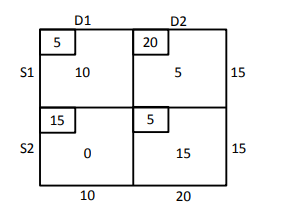
\includegraphics[width=0.75\columnwidth]{chapters/10/7/2/4/figs/fig.png}
 \end{center}
\caption{}
\label{fig:10/7/2/4Fig1}
\end{figure}
\fi

\item Find the position vector of the mid point of the vector joining the points $\vec{P}$(2, 3, 4)
and $\vec{Q}$(4, 1, –2).
\\
\solution
		\begin{enumerate}[label=\thesubsection.\arabic*,ref=\thesubsection.\theenumi]
\item Find the coordinates of the point which divides the join of $(-1,7) $ and $ (4,-3)$ in the ratio 2:3.
	\\
		\solution
	\input{chapters/10/7/2/1/section.tex}
\item Find the coordinates of the point $\vec{R}$ on the line segment joining the points $\vec{P}(-1,3)$ and $\vec{Q}(2,5)$ such that $PR=\frac{3}{5}PQ$.
\item Find the ratio in which the point $\vec{P}\brak{\frac{3}{4},\frac{5}{12}}$ divides the line segment joining the points $\vec{A}\brak{\frac{1}{2},\frac{3}{2}}$ and $ \vec{B}(2,-5)$.
\item Find the coordinates of the point which divides the line segment joining the points $(4,-3)$ and $(8,5)$ in the ratio $3:1$ internally.
\item Find the coordinates of the point $\vec{P}$ on $AD$ such that $AP : PD = 2 : 1$.
\item If the point $\vec{P} (2, 1)$ lies on the line segment joining points $\vec{A} (4, 2)$  and $ \vec{B} (8, 4)$,
then
\begin{enumerate}
	\item $AP =\frac{1}{3}{AB}$ 
\item ${AP}={PE}$
\item ${PB}=\frac{1}{3}{AB}$
\item${AP}=\frac{1}{2}{AB}$
 \end{enumerate}
\item Find the ratio in which the line segment joining the points $(-3,10)$  and  $(6,-8)$  is divided by $ (-1,6)$.
	\\
		\solution
	\input{chapters/10/7/2/4/section.tex}
\item Find the position vector of the mid point of the vector joining the points $\vec{P}$(2, 3, 4)
and $\vec{Q}$(4, 1, –2).
\\
\solution
		\input{chapters/12/10/2/16/section.tex}
\item Let $\vec{A}(4, 2), \vec{B}(6, 5)$  and $ \vec{C}(1, 4)$ be the vertices of $\triangle ABC$.
\begin{enumerate}
\item If $\vec{A}$ and  $\vec{B}$ are $(-2,-2)$ and  $(2,-4)$, respectively, find the coordinates of $\vec{P}$ such that $AP= \frac {3}{7}AB$  and $ \vec{P}$ lies on the line segment $AB$.
	\\
		\solution
	\input{chapters/10/7/2/8/section.tex}
\item Find the coordinates of the points which divide the line segment joining $A(-2,2)$  and  $\vec{B}(2,8)$ into four equal parts.
	\\
		\solution
	\input{chapters/10/7/2/9/section.tex}
\item In what ratio does the point $(-4,6)$ divide the line segment joining the points $\vec{A}(-6,0)$ and $\vec{B}(3,-8)$?
\item Given that $\vec{P}(3,2,-4), \vec{Q}(5,4,-6)$ and $\vec{R}(9,8,-10)$ are collinear. Find the ratio in which $\vec{Q}$ divides $PR$.
\item Points $\vec{A}(-6,10),\vec{B}(-4,6)$  and  $\vec{C}(3,-8)$ are collinear such that $AB=  \frac{2}{9}AC$.
\item The point which divides the line segment joining the points $\vec{P} (7, –6) $  and  $\vec{Q}(3, 4)$ in the 
ratio 1 : 2 internally lies in  which quadrant?
\item Find the coordinates of the points of trisection of the line segment joining $(4,-1)$  and  $(-2,3)$.
	\\
		\solution
	\input{chapters/10/7/2/2/section.tex}
\item Find the coordinates of the points which trisect the line segment joining the points $\vec{P}(4,2,-6)$ and $\vec{Q}(10,-16,6)$.
\item Find the coordinates of the points of trisection (i.e. points dividing to three equal parts) of the line segment joining the points $\vec{A}(2,-2)$ and $\vec{B}(-7,4)$.
\item Point $\vec{P}(5,-3)$ is one of the two points of trisection of line segment joining the points $\vec{A}(7,-2)$ and $\vec{B}(1,-5)$
\item Find the position vector of a point $\vec{R}$ which divides the line joining two points $\vec{P}$
and $\vec{Q}$ whose position vectors are $\hat{i}+2\hat{j}-\hat{k}$ and $-\hat{i}+\hat{j}+\hat{k}$ respectively, in the
ratio 2 : 1
\begin{enumerate}
    \item  internally
    \item  externally
\end{enumerate}
%\solution
%		\input{chapters/12/10/2/15/section.tex}
\item Find the coordinates of the point which divides the line segment joining the points which divides the line segment joining  the points $(-2,3,5)$ and $(1,-4,6)$ in the ratio 
\begin{enumerate}
\item $2:3$ internally,
\item $2:3$ externally
\end{enumerate}
\item Find the coordinates of the point which divides the line segment joining the points $(1,-2,3)$ and $(3,4,-5)$ in the ratio $2:3$
\begin{enumerate}
\item internally, and
\item externally
\end{enumerate}
\item Consider two points $\vec{P}$ and $\vec{Q}$ with position vectors $\overrightarrow{OP} = 3\overrightarrow{a}-2\overrightarrow{b}$ and $\overrightarrow{OQ}=\overrightarrow{a}+\overrightarrow{b}$. Find the position vector of a point $\vec{R}$ which divides the line joining $\vec{P}$ and $\vec{Q}$ in the ratio $2:1$, 
\begin{enumerate}
\item internally, and 
\item externally.
\end{enumerate}
\item The median from $\vec{A}$ meets $BC$ at $\vec{D}$. Find the coordinates of the point $\vec{D}$.
\item Find the coordinates of points $\vec{Q}$ and $\vec{R}$ on medians $BE$ and $CF$ respectively such that $BQ : QE = 2 : 1$  and  $CR : RF = 2 : 1$.
\item What do you observe?
\item If $\vec{A}, \vec{B}$ and $\vec{C}$  are the vertices of $\triangle ABC$, find the coordinates of the centroid of the triangle.
\end{enumerate}
\solution
	\input{chapters/10/7/4/7/section.tex}
\item If $\vec{P}(9a-2,-b)$ divides line segment joining $\vec{A}(3a+1,-3)$ and $\vec{B}(8a,5)$ in the ratio 3:1, find the values of $a$ and $b$.
\item Find the position vector of a point $\vec{R}$ which divides the line joining two points $\vec{P}$ and $\vec{Q}$ whose position vectors are $2\vec{a}+\vec{b}$ and $\vec{a}-3\vec{b}$ externally in the ratio $1:2$.
\item The position vector of the point which divides the join of points 2$\vec{a}$-3$\vec{b}$ $\text{and}$ $\vec{a}+\vec{b}$ in the ratio 3:1 is \rule{1cm}{0.1pt}.
\item If $\vec{a}$ and $\vec{b}$ are the postion vectors of $\vec{A}$ and $\vec{B}$, respectively, find the position vector of a point $\vec{C}$ in $BA$ produced such that $BC=1.5BA$.
\item Find the position vector of a point $\vec{R}$ which divides the line joining two points $\vec{P}$ and $\vec{Q}$ whose position vectors are $(2\vec{a}+\vec{b})$ and $(\vec{a}-3\vec{b})$
externally in the ratio 1 : 2. Also, show that $\vec{P}$ is the mid point of the line segment $RQ$.
\end{enumerate}

\item Let $\vec{A}(4, 2), \vec{B}(6, 5)$  and $ \vec{C}(1, 4)$ be the vertices of $\triangle ABC$.
\begin{enumerate}
\item If $\vec{A}$ and  $\vec{B}$ are $(-2,-2)$ and  $(2,-4)$, respectively, find the coordinates of $\vec{P}$ such that $AP= \frac {3}{7}AB$  and $ \vec{P}$ lies on the line segment $AB$.
	\\
		\solution
	\begin{enumerate}[label=\thesubsection.\arabic*,ref=\thesubsection.\theenumi]
\item Find the coordinates of the point which divides the join of $(-1,7) $ and $ (4,-3)$ in the ratio 2:3.
	\\
		\solution
	\input{chapters/10/7/2/1/section.tex}
\item Find the coordinates of the point $\vec{R}$ on the line segment joining the points $\vec{P}(-1,3)$ and $\vec{Q}(2,5)$ such that $PR=\frac{3}{5}PQ$.
\item Find the ratio in which the point $\vec{P}\brak{\frac{3}{4},\frac{5}{12}}$ divides the line segment joining the points $\vec{A}\brak{\frac{1}{2},\frac{3}{2}}$ and $ \vec{B}(2,-5)$.
\item Find the coordinates of the point which divides the line segment joining the points $(4,-3)$ and $(8,5)$ in the ratio $3:1$ internally.
\item Find the coordinates of the point $\vec{P}$ on $AD$ such that $AP : PD = 2 : 1$.
\item If the point $\vec{P} (2, 1)$ lies on the line segment joining points $\vec{A} (4, 2)$  and $ \vec{B} (8, 4)$,
then
\begin{enumerate}
	\item $AP =\frac{1}{3}{AB}$ 
\item ${AP}={PE}$
\item ${PB}=\frac{1}{3}{AB}$
\item${AP}=\frac{1}{2}{AB}$
 \end{enumerate}
\item Find the ratio in which the line segment joining the points $(-3,10)$  and  $(6,-8)$  is divided by $ (-1,6)$.
	\\
		\solution
	\input{chapters/10/7/2/4/section.tex}
\item Find the position vector of the mid point of the vector joining the points $\vec{P}$(2, 3, 4)
and $\vec{Q}$(4, 1, –2).
\\
\solution
		\input{chapters/12/10/2/16/section.tex}
\item Let $\vec{A}(4, 2), \vec{B}(6, 5)$  and $ \vec{C}(1, 4)$ be the vertices of $\triangle ABC$.
\begin{enumerate}
\item If $\vec{A}$ and  $\vec{B}$ are $(-2,-2)$ and  $(2,-4)$, respectively, find the coordinates of $\vec{P}$ such that $AP= \frac {3}{7}AB$  and $ \vec{P}$ lies on the line segment $AB$.
	\\
		\solution
	\input{chapters/10/7/2/8/section.tex}
\item Find the coordinates of the points which divide the line segment joining $A(-2,2)$  and  $\vec{B}(2,8)$ into four equal parts.
	\\
		\solution
	\input{chapters/10/7/2/9/section.tex}
\item In what ratio does the point $(-4,6)$ divide the line segment joining the points $\vec{A}(-6,0)$ and $\vec{B}(3,-8)$?
\item Given that $\vec{P}(3,2,-4), \vec{Q}(5,4,-6)$ and $\vec{R}(9,8,-10)$ are collinear. Find the ratio in which $\vec{Q}$ divides $PR$.
\item Points $\vec{A}(-6,10),\vec{B}(-4,6)$  and  $\vec{C}(3,-8)$ are collinear such that $AB=  \frac{2}{9}AC$.
\item The point which divides the line segment joining the points $\vec{P} (7, –6) $  and  $\vec{Q}(3, 4)$ in the 
ratio 1 : 2 internally lies in  which quadrant?
\item Find the coordinates of the points of trisection of the line segment joining $(4,-1)$  and  $(-2,3)$.
	\\
		\solution
	\input{chapters/10/7/2/2/section.tex}
\item Find the coordinates of the points which trisect the line segment joining the points $\vec{P}(4,2,-6)$ and $\vec{Q}(10,-16,6)$.
\item Find the coordinates of the points of trisection (i.e. points dividing to three equal parts) of the line segment joining the points $\vec{A}(2,-2)$ and $\vec{B}(-7,4)$.
\item Point $\vec{P}(5,-3)$ is one of the two points of trisection of line segment joining the points $\vec{A}(7,-2)$ and $\vec{B}(1,-5)$
\item Find the position vector of a point $\vec{R}$ which divides the line joining two points $\vec{P}$
and $\vec{Q}$ whose position vectors are $\hat{i}+2\hat{j}-\hat{k}$ and $-\hat{i}+\hat{j}+\hat{k}$ respectively, in the
ratio 2 : 1
\begin{enumerate}
    \item  internally
    \item  externally
\end{enumerate}
%\solution
%		\input{chapters/12/10/2/15/section.tex}
\item Find the coordinates of the point which divides the line segment joining the points which divides the line segment joining  the points $(-2,3,5)$ and $(1,-4,6)$ in the ratio 
\begin{enumerate}
\item $2:3$ internally,
\item $2:3$ externally
\end{enumerate}
\item Find the coordinates of the point which divides the line segment joining the points $(1,-2,3)$ and $(3,4,-5)$ in the ratio $2:3$
\begin{enumerate}
\item internally, and
\item externally
\end{enumerate}
\item Consider two points $\vec{P}$ and $\vec{Q}$ with position vectors $\overrightarrow{OP} = 3\overrightarrow{a}-2\overrightarrow{b}$ and $\overrightarrow{OQ}=\overrightarrow{a}+\overrightarrow{b}$. Find the position vector of a point $\vec{R}$ which divides the line joining $\vec{P}$ and $\vec{Q}$ in the ratio $2:1$, 
\begin{enumerate}
\item internally, and 
\item externally.
\end{enumerate}
\item The median from $\vec{A}$ meets $BC$ at $\vec{D}$. Find the coordinates of the point $\vec{D}$.
\item Find the coordinates of points $\vec{Q}$ and $\vec{R}$ on medians $BE$ and $CF$ respectively such that $BQ : QE = 2 : 1$  and  $CR : RF = 2 : 1$.
\item What do you observe?
\item If $\vec{A}, \vec{B}$ and $\vec{C}$  are the vertices of $\triangle ABC$, find the coordinates of the centroid of the triangle.
\end{enumerate}
\solution
	\input{chapters/10/7/4/7/section.tex}
\item If $\vec{P}(9a-2,-b)$ divides line segment joining $\vec{A}(3a+1,-3)$ and $\vec{B}(8a,5)$ in the ratio 3:1, find the values of $a$ and $b$.
\item Find the position vector of a point $\vec{R}$ which divides the line joining two points $\vec{P}$ and $\vec{Q}$ whose position vectors are $2\vec{a}+\vec{b}$ and $\vec{a}-3\vec{b}$ externally in the ratio $1:2$.
\item The position vector of the point which divides the join of points 2$\vec{a}$-3$\vec{b}$ $\text{and}$ $\vec{a}+\vec{b}$ in the ratio 3:1 is \rule{1cm}{0.1pt}.
\item If $\vec{a}$ and $\vec{b}$ are the postion vectors of $\vec{A}$ and $\vec{B}$, respectively, find the position vector of a point $\vec{C}$ in $BA$ produced such that $BC=1.5BA$.
\item Find the position vector of a point $\vec{R}$ which divides the line joining two points $\vec{P}$ and $\vec{Q}$ whose position vectors are $(2\vec{a}+\vec{b})$ and $(\vec{a}-3\vec{b})$
externally in the ratio 1 : 2. Also, show that $\vec{P}$ is the mid point of the line segment $RQ$.
\end{enumerate}

\item Find the coordinates of the points which divide the line segment joining $A(-2,2)$  and  $\vec{B}(2,8)$ into four equal parts.
	\\
		\solution
	\begin{enumerate}[label=\thesubsection.\arabic*,ref=\thesubsection.\theenumi]
\item Find the coordinates of the point which divides the join of $(-1,7) $ and $ (4,-3)$ in the ratio 2:3.
	\\
		\solution
	\input{chapters/10/7/2/1/section.tex}
\item Find the coordinates of the point $\vec{R}$ on the line segment joining the points $\vec{P}(-1,3)$ and $\vec{Q}(2,5)$ such that $PR=\frac{3}{5}PQ$.
\item Find the ratio in which the point $\vec{P}\brak{\frac{3}{4},\frac{5}{12}}$ divides the line segment joining the points $\vec{A}\brak{\frac{1}{2},\frac{3}{2}}$ and $ \vec{B}(2,-5)$.
\item Find the coordinates of the point which divides the line segment joining the points $(4,-3)$ and $(8,5)$ in the ratio $3:1$ internally.
\item Find the coordinates of the point $\vec{P}$ on $AD$ such that $AP : PD = 2 : 1$.
\item If the point $\vec{P} (2, 1)$ lies on the line segment joining points $\vec{A} (4, 2)$  and $ \vec{B} (8, 4)$,
then
\begin{enumerate}
	\item $AP =\frac{1}{3}{AB}$ 
\item ${AP}={PE}$
\item ${PB}=\frac{1}{3}{AB}$
\item${AP}=\frac{1}{2}{AB}$
 \end{enumerate}
\item Find the ratio in which the line segment joining the points $(-3,10)$  and  $(6,-8)$  is divided by $ (-1,6)$.
	\\
		\solution
	\input{chapters/10/7/2/4/section.tex}
\item Find the position vector of the mid point of the vector joining the points $\vec{P}$(2, 3, 4)
and $\vec{Q}$(4, 1, –2).
\\
\solution
		\input{chapters/12/10/2/16/section.tex}
\item Let $\vec{A}(4, 2), \vec{B}(6, 5)$  and $ \vec{C}(1, 4)$ be the vertices of $\triangle ABC$.
\begin{enumerate}
\item If $\vec{A}$ and  $\vec{B}$ are $(-2,-2)$ and  $(2,-4)$, respectively, find the coordinates of $\vec{P}$ such that $AP= \frac {3}{7}AB$  and $ \vec{P}$ lies on the line segment $AB$.
	\\
		\solution
	\input{chapters/10/7/2/8/section.tex}
\item Find the coordinates of the points which divide the line segment joining $A(-2,2)$  and  $\vec{B}(2,8)$ into four equal parts.
	\\
		\solution
	\input{chapters/10/7/2/9/section.tex}
\item In what ratio does the point $(-4,6)$ divide the line segment joining the points $\vec{A}(-6,0)$ and $\vec{B}(3,-8)$?
\item Given that $\vec{P}(3,2,-4), \vec{Q}(5,4,-6)$ and $\vec{R}(9,8,-10)$ are collinear. Find the ratio in which $\vec{Q}$ divides $PR$.
\item Points $\vec{A}(-6,10),\vec{B}(-4,6)$  and  $\vec{C}(3,-8)$ are collinear such that $AB=  \frac{2}{9}AC$.
\item The point which divides the line segment joining the points $\vec{P} (7, –6) $  and  $\vec{Q}(3, 4)$ in the 
ratio 1 : 2 internally lies in  which quadrant?
\item Find the coordinates of the points of trisection of the line segment joining $(4,-1)$  and  $(-2,3)$.
	\\
		\solution
	\input{chapters/10/7/2/2/section.tex}
\item Find the coordinates of the points which trisect the line segment joining the points $\vec{P}(4,2,-6)$ and $\vec{Q}(10,-16,6)$.
\item Find the coordinates of the points of trisection (i.e. points dividing to three equal parts) of the line segment joining the points $\vec{A}(2,-2)$ and $\vec{B}(-7,4)$.
\item Point $\vec{P}(5,-3)$ is one of the two points of trisection of line segment joining the points $\vec{A}(7,-2)$ and $\vec{B}(1,-5)$
\item Find the position vector of a point $\vec{R}$ which divides the line joining two points $\vec{P}$
and $\vec{Q}$ whose position vectors are $\hat{i}+2\hat{j}-\hat{k}$ and $-\hat{i}+\hat{j}+\hat{k}$ respectively, in the
ratio 2 : 1
\begin{enumerate}
    \item  internally
    \item  externally
\end{enumerate}
%\solution
%		\input{chapters/12/10/2/15/section.tex}
\item Find the coordinates of the point which divides the line segment joining the points which divides the line segment joining  the points $(-2,3,5)$ and $(1,-4,6)$ in the ratio 
\begin{enumerate}
\item $2:3$ internally,
\item $2:3$ externally
\end{enumerate}
\item Find the coordinates of the point which divides the line segment joining the points $(1,-2,3)$ and $(3,4,-5)$ in the ratio $2:3$
\begin{enumerate}
\item internally, and
\item externally
\end{enumerate}
\item Consider two points $\vec{P}$ and $\vec{Q}$ with position vectors $\overrightarrow{OP} = 3\overrightarrow{a}-2\overrightarrow{b}$ and $\overrightarrow{OQ}=\overrightarrow{a}+\overrightarrow{b}$. Find the position vector of a point $\vec{R}$ which divides the line joining $\vec{P}$ and $\vec{Q}$ in the ratio $2:1$, 
\begin{enumerate}
\item internally, and 
\item externally.
\end{enumerate}
\item The median from $\vec{A}$ meets $BC$ at $\vec{D}$. Find the coordinates of the point $\vec{D}$.
\item Find the coordinates of points $\vec{Q}$ and $\vec{R}$ on medians $BE$ and $CF$ respectively such that $BQ : QE = 2 : 1$  and  $CR : RF = 2 : 1$.
\item What do you observe?
\item If $\vec{A}, \vec{B}$ and $\vec{C}$  are the vertices of $\triangle ABC$, find the coordinates of the centroid of the triangle.
\end{enumerate}
\solution
	\input{chapters/10/7/4/7/section.tex}
\item If $\vec{P}(9a-2,-b)$ divides line segment joining $\vec{A}(3a+1,-3)$ and $\vec{B}(8a,5)$ in the ratio 3:1, find the values of $a$ and $b$.
\item Find the position vector of a point $\vec{R}$ which divides the line joining two points $\vec{P}$ and $\vec{Q}$ whose position vectors are $2\vec{a}+\vec{b}$ and $\vec{a}-3\vec{b}$ externally in the ratio $1:2$.
\item The position vector of the point which divides the join of points 2$\vec{a}$-3$\vec{b}$ $\text{and}$ $\vec{a}+\vec{b}$ in the ratio 3:1 is \rule{1cm}{0.1pt}.
\item If $\vec{a}$ and $\vec{b}$ are the postion vectors of $\vec{A}$ and $\vec{B}$, respectively, find the position vector of a point $\vec{C}$ in $BA$ produced such that $BC=1.5BA$.
\item Find the position vector of a point $\vec{R}$ which divides the line joining two points $\vec{P}$ and $\vec{Q}$ whose position vectors are $(2\vec{a}+\vec{b})$ and $(\vec{a}-3\vec{b})$
externally in the ratio 1 : 2. Also, show that $\vec{P}$ is the mid point of the line segment $RQ$.
\end{enumerate}

\item In what ratio does the point $(-4,6)$ divide the line segment joining the points $\vec{A}(-6,0)$ and $\vec{B}(3,-8)$?
\item Given that $\vec{P}(3,2,-4), \vec{Q}(5,4,-6)$ and $\vec{R}(9,8,-10)$ are collinear. Find the ratio in which $\vec{Q}$ divides $PR$.
\item Points $\vec{A}(-6,10),\vec{B}(-4,6)$  and  $\vec{C}(3,-8)$ are collinear such that $AB=  \frac{2}{9}AC$.
\item The point which divides the line segment joining the points $\vec{P} (7, –6) $  and  $\vec{Q}(3, 4)$ in the 
ratio 1 : 2 internally lies in  which quadrant?
\item Find the coordinates of the points of trisection of the line segment joining $(4,-1)$  and  $(-2,3)$.
	\\
		\solution
	Using section formula,
\begin{align}
\vec{R}=\frac{1}{1+\frac{1}{2}}\brak{\myvec{4\\-1}+\frac{1}{2}\myvec{-2\\3}}
=\myvec{2\\ \frac{1}{3}}\\
\vec{S}=\frac{1}{1+\frac{2}{1}}\brak{\myvec{4\\-1}+\frac{2}{1}\myvec{-2\\3}}
=\myvec{0\\ \frac{5}{3}}
\end{align}
which are the desired points of trisection.
\iffalse
See
		\figref{fig:chapters/10/7/2/2/Figure}
\begin{figure}[H]
\centering
\includegraphics[width=0.75\columnwidth]{chapters/10/7/2/2/figs/dj.pdf}
\caption{}
		\label{fig:chapters/10/7/2/2/Figure}
\end{figure}
\fi

\item Find the coordinates of the points which trisect the line segment joining the points $\vec{P}(4,2,-6)$ and $\vec{Q}(10,-16,6)$.
\item Find the coordinates of the points of trisection (i.e. points dividing to three equal parts) of the line segment joining the points $\vec{A}(2,-2)$ and $\vec{B}(-7,4)$.
\item Point $\vec{P}(5,-3)$ is one of the two points of trisection of line segment joining the points $\vec{A}(7,-2)$ and $\vec{B}(1,-5)$
\item Find the position vector of a point $\vec{R}$ which divides the line joining two points $\vec{P}$
and $\vec{Q}$ whose position vectors are $\hat{i}+2\hat{j}-\hat{k}$ and $-\hat{i}+\hat{j}+\hat{k}$ respectively, in the
ratio 2 : 1
\begin{enumerate}
    \item  internally
    \item  externally
\end{enumerate}
%\solution
%		\begin{enumerate}[label=\thesubsection.\arabic*,ref=\thesubsection.\theenumi]
\item Find the coordinates of the point which divides the join of $(-1,7) $ and $ (4,-3)$ in the ratio 2:3.
	\\
		\solution
	\input{chapters/10/7/2/1/section.tex}
\item Find the coordinates of the point $\vec{R}$ on the line segment joining the points $\vec{P}(-1,3)$ and $\vec{Q}(2,5)$ such that $PR=\frac{3}{5}PQ$.
\item Find the ratio in which the point $\vec{P}\brak{\frac{3}{4},\frac{5}{12}}$ divides the line segment joining the points $\vec{A}\brak{\frac{1}{2},\frac{3}{2}}$ and $ \vec{B}(2,-5)$.
\item Find the coordinates of the point which divides the line segment joining the points $(4,-3)$ and $(8,5)$ in the ratio $3:1$ internally.
\item Find the coordinates of the point $\vec{P}$ on $AD$ such that $AP : PD = 2 : 1$.
\item If the point $\vec{P} (2, 1)$ lies on the line segment joining points $\vec{A} (4, 2)$  and $ \vec{B} (8, 4)$,
then
\begin{enumerate}
	\item $AP =\frac{1}{3}{AB}$ 
\item ${AP}={PE}$
\item ${PB}=\frac{1}{3}{AB}$
\item${AP}=\frac{1}{2}{AB}$
 \end{enumerate}
\item Find the ratio in which the line segment joining the points $(-3,10)$  and  $(6,-8)$  is divided by $ (-1,6)$.
	\\
		\solution
	\input{chapters/10/7/2/4/section.tex}
\item Find the position vector of the mid point of the vector joining the points $\vec{P}$(2, 3, 4)
and $\vec{Q}$(4, 1, –2).
\\
\solution
		\input{chapters/12/10/2/16/section.tex}
\item Let $\vec{A}(4, 2), \vec{B}(6, 5)$  and $ \vec{C}(1, 4)$ be the vertices of $\triangle ABC$.
\begin{enumerate}
\item If $\vec{A}$ and  $\vec{B}$ are $(-2,-2)$ and  $(2,-4)$, respectively, find the coordinates of $\vec{P}$ such that $AP= \frac {3}{7}AB$  and $ \vec{P}$ lies on the line segment $AB$.
	\\
		\solution
	\input{chapters/10/7/2/8/section.tex}
\item Find the coordinates of the points which divide the line segment joining $A(-2,2)$  and  $\vec{B}(2,8)$ into four equal parts.
	\\
		\solution
	\input{chapters/10/7/2/9/section.tex}
\item In what ratio does the point $(-4,6)$ divide the line segment joining the points $\vec{A}(-6,0)$ and $\vec{B}(3,-8)$?
\item Given that $\vec{P}(3,2,-4), \vec{Q}(5,4,-6)$ and $\vec{R}(9,8,-10)$ are collinear. Find the ratio in which $\vec{Q}$ divides $PR$.
\item Points $\vec{A}(-6,10),\vec{B}(-4,6)$  and  $\vec{C}(3,-8)$ are collinear such that $AB=  \frac{2}{9}AC$.
\item The point which divides the line segment joining the points $\vec{P} (7, –6) $  and  $\vec{Q}(3, 4)$ in the 
ratio 1 : 2 internally lies in  which quadrant?
\item Find the coordinates of the points of trisection of the line segment joining $(4,-1)$  and  $(-2,3)$.
	\\
		\solution
	\input{chapters/10/7/2/2/section.tex}
\item Find the coordinates of the points which trisect the line segment joining the points $\vec{P}(4,2,-6)$ and $\vec{Q}(10,-16,6)$.
\item Find the coordinates of the points of trisection (i.e. points dividing to three equal parts) of the line segment joining the points $\vec{A}(2,-2)$ and $\vec{B}(-7,4)$.
\item Point $\vec{P}(5,-3)$ is one of the two points of trisection of line segment joining the points $\vec{A}(7,-2)$ and $\vec{B}(1,-5)$
\item Find the position vector of a point $\vec{R}$ which divides the line joining two points $\vec{P}$
and $\vec{Q}$ whose position vectors are $\hat{i}+2\hat{j}-\hat{k}$ and $-\hat{i}+\hat{j}+\hat{k}$ respectively, in the
ratio 2 : 1
\begin{enumerate}
    \item  internally
    \item  externally
\end{enumerate}
%\solution
%		\input{chapters/12/10/2/15/section.tex}
\item Find the coordinates of the point which divides the line segment joining the points which divides the line segment joining  the points $(-2,3,5)$ and $(1,-4,6)$ in the ratio 
\begin{enumerate}
\item $2:3$ internally,
\item $2:3$ externally
\end{enumerate}
\item Find the coordinates of the point which divides the line segment joining the points $(1,-2,3)$ and $(3,4,-5)$ in the ratio $2:3$
\begin{enumerate}
\item internally, and
\item externally
\end{enumerate}
\item Consider two points $\vec{P}$ and $\vec{Q}$ with position vectors $\overrightarrow{OP} = 3\overrightarrow{a}-2\overrightarrow{b}$ and $\overrightarrow{OQ}=\overrightarrow{a}+\overrightarrow{b}$. Find the position vector of a point $\vec{R}$ which divides the line joining $\vec{P}$ and $\vec{Q}$ in the ratio $2:1$, 
\begin{enumerate}
\item internally, and 
\item externally.
\end{enumerate}
\item The median from $\vec{A}$ meets $BC$ at $\vec{D}$. Find the coordinates of the point $\vec{D}$.
\item Find the coordinates of points $\vec{Q}$ and $\vec{R}$ on medians $BE$ and $CF$ respectively such that $BQ : QE = 2 : 1$  and  $CR : RF = 2 : 1$.
\item What do you observe?
\item If $\vec{A}, \vec{B}$ and $\vec{C}$  are the vertices of $\triangle ABC$, find the coordinates of the centroid of the triangle.
\end{enumerate}
\solution
	\input{chapters/10/7/4/7/section.tex}
\item If $\vec{P}(9a-2,-b)$ divides line segment joining $\vec{A}(3a+1,-3)$ and $\vec{B}(8a,5)$ in the ratio 3:1, find the values of $a$ and $b$.
\item Find the position vector of a point $\vec{R}$ which divides the line joining two points $\vec{P}$ and $\vec{Q}$ whose position vectors are $2\vec{a}+\vec{b}$ and $\vec{a}-3\vec{b}$ externally in the ratio $1:2$.
\item The position vector of the point which divides the join of points 2$\vec{a}$-3$\vec{b}$ $\text{and}$ $\vec{a}+\vec{b}$ in the ratio 3:1 is \rule{1cm}{0.1pt}.
\item If $\vec{a}$ and $\vec{b}$ are the postion vectors of $\vec{A}$ and $\vec{B}$, respectively, find the position vector of a point $\vec{C}$ in $BA$ produced such that $BC=1.5BA$.
\item Find the position vector of a point $\vec{R}$ which divides the line joining two points $\vec{P}$ and $\vec{Q}$ whose position vectors are $(2\vec{a}+\vec{b})$ and $(\vec{a}-3\vec{b})$
externally in the ratio 1 : 2. Also, show that $\vec{P}$ is the mid point of the line segment $RQ$.
\end{enumerate}

\item Find the coordinates of the point which divides the line segment joining the points which divides the line segment joining  the points $(-2,3,5)$ and $(1,-4,6)$ in the ratio 
\begin{enumerate}
\item $2:3$ internally,
\item $2:3$ externally
\end{enumerate}
\item Find the coordinates of the point which divides the line segment joining the points $(1,-2,3)$ and $(3,4,-5)$ in the ratio $2:3$
\begin{enumerate}
\item internally, and
\item externally
\end{enumerate}
\item Consider two points $\vec{P}$ and $\vec{Q}$ with position vectors $\overrightarrow{OP} = 3\overrightarrow{a}-2\overrightarrow{b}$ and $\overrightarrow{OQ}=\overrightarrow{a}+\overrightarrow{b}$. Find the position vector of a point $\vec{R}$ which divides the line joining $\vec{P}$ and $\vec{Q}$ in the ratio $2:1$, 
\begin{enumerate}
\item internally, and 
\item externally.
\end{enumerate}
\item The median from $\vec{A}$ meets $BC$ at $\vec{D}$. Find the coordinates of the point $\vec{D}$.
\item Find the coordinates of points $\vec{Q}$ and $\vec{R}$ on medians $BE$ and $CF$ respectively such that $BQ : QE = 2 : 1$  and  $CR : RF = 2 : 1$.
\item What do you observe?
\item If $\vec{A}, \vec{B}$ and $\vec{C}$  are the vertices of $\triangle ABC$, find the coordinates of the centroid of the triangle.
\end{enumerate}
\solution
	\begin{enumerate}[label=\thesubsection.\arabic*,ref=\thesubsection.\theenumi]
\item Find the coordinates of the point which divides the join of $(-1,7) $ and $ (4,-3)$ in the ratio 2:3.
	\\
		\solution
	\input{chapters/10/7/2/1/section.tex}
\item Find the coordinates of the point $\vec{R}$ on the line segment joining the points $\vec{P}(-1,3)$ and $\vec{Q}(2,5)$ such that $PR=\frac{3}{5}PQ$.
\item Find the ratio in which the point $\vec{P}\brak{\frac{3}{4},\frac{5}{12}}$ divides the line segment joining the points $\vec{A}\brak{\frac{1}{2},\frac{3}{2}}$ and $ \vec{B}(2,-5)$.
\item Find the coordinates of the point which divides the line segment joining the points $(4,-3)$ and $(8,5)$ in the ratio $3:1$ internally.
\item Find the coordinates of the point $\vec{P}$ on $AD$ such that $AP : PD = 2 : 1$.
\item If the point $\vec{P} (2, 1)$ lies on the line segment joining points $\vec{A} (4, 2)$  and $ \vec{B} (8, 4)$,
then
\begin{enumerate}
	\item $AP =\frac{1}{3}{AB}$ 
\item ${AP}={PE}$
\item ${PB}=\frac{1}{3}{AB}$
\item${AP}=\frac{1}{2}{AB}$
 \end{enumerate}
\item Find the ratio in which the line segment joining the points $(-3,10)$  and  $(6,-8)$  is divided by $ (-1,6)$.
	\\
		\solution
	\input{chapters/10/7/2/4/section.tex}
\item Find the position vector of the mid point of the vector joining the points $\vec{P}$(2, 3, 4)
and $\vec{Q}$(4, 1, –2).
\\
\solution
		\input{chapters/12/10/2/16/section.tex}
\item Let $\vec{A}(4, 2), \vec{B}(6, 5)$  and $ \vec{C}(1, 4)$ be the vertices of $\triangle ABC$.
\begin{enumerate}
\item If $\vec{A}$ and  $\vec{B}$ are $(-2,-2)$ and  $(2,-4)$, respectively, find the coordinates of $\vec{P}$ such that $AP= \frac {3}{7}AB$  and $ \vec{P}$ lies on the line segment $AB$.
	\\
		\solution
	\input{chapters/10/7/2/8/section.tex}
\item Find the coordinates of the points which divide the line segment joining $A(-2,2)$  and  $\vec{B}(2,8)$ into four equal parts.
	\\
		\solution
	\input{chapters/10/7/2/9/section.tex}
\item In what ratio does the point $(-4,6)$ divide the line segment joining the points $\vec{A}(-6,0)$ and $\vec{B}(3,-8)$?
\item Given that $\vec{P}(3,2,-4), \vec{Q}(5,4,-6)$ and $\vec{R}(9,8,-10)$ are collinear. Find the ratio in which $\vec{Q}$ divides $PR$.
\item Points $\vec{A}(-6,10),\vec{B}(-4,6)$  and  $\vec{C}(3,-8)$ are collinear such that $AB=  \frac{2}{9}AC$.
\item The point which divides the line segment joining the points $\vec{P} (7, –6) $  and  $\vec{Q}(3, 4)$ in the 
ratio 1 : 2 internally lies in  which quadrant?
\item Find the coordinates of the points of trisection of the line segment joining $(4,-1)$  and  $(-2,3)$.
	\\
		\solution
	\input{chapters/10/7/2/2/section.tex}
\item Find the coordinates of the points which trisect the line segment joining the points $\vec{P}(4,2,-6)$ and $\vec{Q}(10,-16,6)$.
\item Find the coordinates of the points of trisection (i.e. points dividing to three equal parts) of the line segment joining the points $\vec{A}(2,-2)$ and $\vec{B}(-7,4)$.
\item Point $\vec{P}(5,-3)$ is one of the two points of trisection of line segment joining the points $\vec{A}(7,-2)$ and $\vec{B}(1,-5)$
\item Find the position vector of a point $\vec{R}$ which divides the line joining two points $\vec{P}$
and $\vec{Q}$ whose position vectors are $\hat{i}+2\hat{j}-\hat{k}$ and $-\hat{i}+\hat{j}+\hat{k}$ respectively, in the
ratio 2 : 1
\begin{enumerate}
    \item  internally
    \item  externally
\end{enumerate}
%\solution
%		\input{chapters/12/10/2/15/section.tex}
\item Find the coordinates of the point which divides the line segment joining the points which divides the line segment joining  the points $(-2,3,5)$ and $(1,-4,6)$ in the ratio 
\begin{enumerate}
\item $2:3$ internally,
\item $2:3$ externally
\end{enumerate}
\item Find the coordinates of the point which divides the line segment joining the points $(1,-2,3)$ and $(3,4,-5)$ in the ratio $2:3$
\begin{enumerate}
\item internally, and
\item externally
\end{enumerate}
\item Consider two points $\vec{P}$ and $\vec{Q}$ with position vectors $\overrightarrow{OP} = 3\overrightarrow{a}-2\overrightarrow{b}$ and $\overrightarrow{OQ}=\overrightarrow{a}+\overrightarrow{b}$. Find the position vector of a point $\vec{R}$ which divides the line joining $\vec{P}$ and $\vec{Q}$ in the ratio $2:1$, 
\begin{enumerate}
\item internally, and 
\item externally.
\end{enumerate}
\item The median from $\vec{A}$ meets $BC$ at $\vec{D}$. Find the coordinates of the point $\vec{D}$.
\item Find the coordinates of points $\vec{Q}$ and $\vec{R}$ on medians $BE$ and $CF$ respectively such that $BQ : QE = 2 : 1$  and  $CR : RF = 2 : 1$.
\item What do you observe?
\item If $\vec{A}, \vec{B}$ and $\vec{C}$  are the vertices of $\triangle ABC$, find the coordinates of the centroid of the triangle.
\end{enumerate}
\solution
	\input{chapters/10/7/4/7/section.tex}
\item If $\vec{P}(9a-2,-b)$ divides line segment joining $\vec{A}(3a+1,-3)$ and $\vec{B}(8a,5)$ in the ratio 3:1, find the values of $a$ and $b$.
\item Find the position vector of a point $\vec{R}$ which divides the line joining two points $\vec{P}$ and $\vec{Q}$ whose position vectors are $2\vec{a}+\vec{b}$ and $\vec{a}-3\vec{b}$ externally in the ratio $1:2$.
\item The position vector of the point which divides the join of points 2$\vec{a}$-3$\vec{b}$ $\text{and}$ $\vec{a}+\vec{b}$ in the ratio 3:1 is \rule{1cm}{0.1pt}.
\item If $\vec{a}$ and $\vec{b}$ are the postion vectors of $\vec{A}$ and $\vec{B}$, respectively, find the position vector of a point $\vec{C}$ in $BA$ produced such that $BC=1.5BA$.
\item Find the position vector of a point $\vec{R}$ which divides the line joining two points $\vec{P}$ and $\vec{Q}$ whose position vectors are $(2\vec{a}+\vec{b})$ and $(\vec{a}-3\vec{b})$
externally in the ratio 1 : 2. Also, show that $\vec{P}$ is the mid point of the line segment $RQ$.
\end{enumerate}

\item If $\vec{P}(9a-2,-b)$ divides line segment joining $\vec{A}(3a+1,-3)$ and $\vec{B}(8a,5)$ in the ratio 3:1, find the values of $a$ and $b$.
\item Find the position vector of a point $\vec{R}$ which divides the line joining two points $\vec{P}$ and $\vec{Q}$ whose position vectors are $2\vec{a}+\vec{b}$ and $\vec{a}-3\vec{b}$ externally in the ratio $1:2$.
\item The position vector of the point which divides the join of points 2$\vec{a}$-3$\vec{b}$ $\text{and}$ $\vec{a}+\vec{b}$ in the ratio 3:1 is \rule{1cm}{0.1pt}.
\item If $\vec{a}$ and $\vec{b}$ are the postion vectors of $\vec{A}$ and $\vec{B}$, respectively, find the position vector of a point $\vec{C}$ in $BA$ produced such that $BC=1.5BA$.
\item Find the position vector of a point $\vec{R}$ which divides the line joining two points $\vec{P}$ and $\vec{Q}$ whose position vectors are $(2\vec{a}+\vec{b})$ and $(\vec{a}-3\vec{b})$
externally in the ratio 1 : 2. Also, show that $\vec{P}$ is the mid point of the line segment $RQ$.
\end{enumerate}

\item If $\vec{P}(9a-2,-b)$ divides line segment joining $\vec{A}(3a+1,-3)$ and $\vec{B}(8a,5)$ in the ratio 3:1, find the values of $a$ and $b$.
\item Find the position vector of a point $\vec{R}$ which divides the line joining two points $\vec{P}$ and $\vec{Q}$ whose position vectors are $2\vec{a}+\vec{b}$ and $\vec{a}-3\vec{b}$ externally in the ratio $1:2$.
\item The position vector of the point which divides the join of points 2$\vec{a}$-3$\vec{b}$ $\text{and}$ $\vec{a}+\vec{b}$ in the ratio 3:1 is \rule{1cm}{0.1pt}.
\item If $\vec{a}$ and $\vec{b}$ are the postion vectors of $\vec{A}$ and $\vec{B}$, respectively, find the position vector of a point $\vec{C}$ in $BA$ produced such that $BC=1.5BA$.
\item Find the position vector of a point $\vec{R}$ which divides the line joining two points $\vec{P}$ and $\vec{Q}$ whose position vectors are $(2\vec{a}+\vec{b})$ and $(\vec{a}-3\vec{b})$
externally in the ratio 1 : 2. Also, show that $\vec{P}$ is the mid point of the line segment $RQ$.
\end{enumerate}

\item The Fahrenheit temperature $F$ and  absolute temperature $K$ satisfy a linear equation. Given that $K=273$ when $F=32$ and that $K=373$ when $F=212$. Express $K$ in terms of $F$ and find the value of $F$, when $K=0$.
\item A line is such that its segment between the lines $5x-y+4=0$ and $3x+4y-4=0$ is bisected at the point $(1,5)$. Obtain its equation.
\item Find the vector equations of the plane passing through the points $R(2, 5, -3), S(-2, -3, 5)$ and $T(5, 3, -3)$.
\item Find the equation of the plane with intercepts $2, 3$ and $4$ on the x, y and z - axis respectively.
\item Show that the lines 
\begin{align}
\frac{x-a+d}{\alpha -\delta} =\frac{y-a}{\alpha} =\frac{z-a-d}{\alpha +\delta}\\
 \text{  and } 
	\\
	\frac{x-a+c}{\beta -\gamma} =\frac{y -b}{\beta} =\frac{z-b-c}{\beta +\gamma} 
\end{align}
 are coplanar.
\item Show that the lines 
\begin{align}
\frac{x+3}{-3}= \frac{y-1}{1}= \frac{z-5}{5} \text{ and } 
	\\
	\frac{x+1}{-1} =\frac{y-2}{2} =\frac{z-5}{5}. 
\end{align}
are coplanar.
\item Find the equation for the line passing through the points $(-1, 0, 2)$ and $(3, 4, 6)$.
\item The Cartesian equation of a line is
\begin{align}
\frac{x+3}{2}= \frac{y-5}{4}= \frac{z+6}{2}
\end{align} 
Find the vector equation for the line.
\end{enumerate}
